\documentclass[12pt,letterpaper]{report}
\usepackage{natbib}
\usepackage{bm}
\usepackage{bbm}
\usepackage{booktabs}
\usepackage{tikz}
\usetikzlibrary{arrows,positioning,shapes,fit,calc}
\pgfdeclarelayer{background}
\pgfsetlayers{background,main}
\usepackage{multirow}
\usepackage{listings}
\usepackage{color}
\usepackage{float}
\usepackage{graphicx}
\usepackage[figuresleft]{rotating}

\definecolor{dkgreen}{rgb}{0,0.6,0}
\definecolor{gray}{rgb}{0.5,0.5,0.5}
\definecolor{mauve}{rgb}{0.58,0,0.82}
\lstdefinelanguage{Renhanced}%
  {keywords={abbreviate,abline,abs,acos,acosh,action,add1,add,%
      aggregate,alias,Alias,alist,all,anova,any,aov,aperm,append,apply,%
      approx,approxfun,apropos,Arg,args,array,arrows,as,asin,asinh,%
      atan,atan2,atanh,attach,attr,attributes,autoload,autoloader,ave,%
      axis,backsolve,barplot,basename,besselI,besselJ,besselK,besselY,%
      beta,binomial,body,box,boxplot,break,browser,bug,builtins,bxp,by,%
      c,C,call,Call,case,cat,category,cbind,ceiling,character,char,%
      charmatch,check,chol,chol2inv,choose,chull,class,close,cm,codes,%
      coef,coefficients,co,col,colnames,colors,colours,commandArgs,%
      comment,complete,complex,conflicts,Conj,contents,contour,%
      contrasts,contr,control,helmert,contrib,convolve,cooks,coords,%
      distance,coplot,cor,cos,cosh,count,fields,cov,covratio,wt,CRAN,%
      create,crossprod,cummax,cummin,cumprod,cumsum,curve,cut,cycle,D,%
      data,dataentry,date,dbeta,dbinom,dcauchy,dchisq,de,debug,%
      debugger,Defunct,default,delay,delete,deltat,demo,de,density,%
      deparse,dependencies,Deprecated,deriv,description,detach,%
      dev2bitmap,dev,cur,deviance,off,prev,,dexp,df,dfbetas,dffits,%
      dgamma,dgeom,dget,dhyper,diag,diff,digamma,dim,dimnames,dir,%
      dirname,dlnorm,dlogis,dnbinom,dnchisq,dnorm,do,dotplot,double,%
      download,dpois,dput,drop,drop1,dsignrank,dt,dummy,dump,dunif,%
      duplicated,dweibull,dwilcox,dyn,edit,eff,effects,eigen,else,%
      emacs,end,environment,env,erase,eval,equal,evalq,example,exists,%
      exit,exp,expand,expression,External,extract,extractAIC,factor,%
      fail,family,fft,file,filled,find,fitted,fivenum,fix,floor,for,%
      For,formals,format,formatC,formula,Fortran,forwardsolve,frame,%
      frequency,ftable,ftable2table,function,gamma,Gamma,gammaCody,%
      gaussian,gc,gcinfo,gctorture,get,getenv,geterrmessage,getOption,%
      getwd,gl,glm,globalenv,gnome,GNOME,graphics,gray,grep,grey,grid,%
      gsub,hasTsp,hat,heat,help,hist,home,hsv,httpclient,I,identify,if,%
      ifelse,Im,image,\%in\%,index,influence,measures,inherits,install,%
      installed,integer,interaction,interactive,Internal,intersect,%
      inverse,invisible,IQR,is,jitter,kappa,kronecker,labels,lapply,%
      layout,lbeta,lchoose,lcm,legend,length,levels,lgamma,library,%
      licence,license,lines,list,lm,load,local,locator,log,log10,log1p,%
      log2,logical,loglin,lower,lowess,ls,lsfit,lsf,ls,machine,Machine,%
      mad,mahalanobis,make,link,margin,match,Math,matlines,mat,matplot,%
      matpoints,matrix,max,mean,median,memory,menu,merge,methods,min,%
      missing,Mod,mode,model,response,mosaicplot,mtext,mvfft,na,nan,%
      names,omit,nargs,nchar,ncol,NCOL,new,next,NextMethod,nextn,%
      nlevels,nlm,noquote,NotYetImplemented,NotYetUsed,nrow,NROW,null,%
      numeric,\%o\%,objects,offset,old,on,Ops,optim,optimise,optimize,%
      options,or,order,ordered,outer,package,packages,page,pairlist,%
      pairs,palette,panel,par,parent,parse,paste,path,pbeta,pbinom,%
      pcauchy,pchisq,pentagamma,persp,pexp,pf,pgamma,pgeom,phyper,pico,%
      pictex,piechart,Platform,plnorm,plogis,plot,pmatch,pmax,pmin,%
      pnbinom,pnchisq,pnorm,points,poisson,poly,polygon,polyroot,pos,%
      postscript,power,ppoints,ppois,predict,preplot,pretty,Primitive,%
      print,prmatrix,proc,prod,profile,proj,prompt,prop,provide,%
      psignrank,ps,pt,ptukey,punif,pweibull,pwilcox,q,qbeta,qbinom,%
      qcauchy,qchisq,qexp,qf,qgamma,qgeom,qhyper,qlnorm,qlogis,qnbinom,%
      qnchisq,qnorm,qpois,qqline,qqnorm,qqplot,qr,Q,qty,qy,qsignrank,%
      qt,qtukey,quantile,quasi,quit,qunif,quote,qweibull,qwilcox,%
      rainbow,range,rank,rbeta,rbind,rbinom,rcauchy,rchisq,Re,read,csv,%
      csv2,fwf,readline,socket,real,Recall,rect,reformulate,regexpr,%
      relevel,remove,rep,repeat,replace,replications,report,require,%
      resid,residuals,restart,return,rev,rexp,rf,rgamma,rgb,rgeom,R,%
      rhyper,rle,rlnorm,rlogis,rm,rnbinom,RNGkind,rnorm,round,row,%
      rownames,rowsum,rpois,rsignrank,rstandard,rstudent,rt,rug,runif,%
      rweibull,rwilcox,sample,sapply,save,scale,scan,scan,screen,sd,se,%
      search,searchpaths,segments,seq,sequence,setdiff,setequal,set,%
      setwd,show,sign,signif,sin,single,sinh,sink,solve,sort,source,%
      spline,splinefun,split,sqrt,stars,start,stat,stem,step,stop,%
      storage,strstrheight,stripplot,strsplit,structure,strwidth,sub,%
      subset,substitute,substr,substring,sum,summary,sunflowerplot,svd,%
      sweep,switch,symbol,symbols,symnum,sys,status,system,t,table,%
      tabulate,tan,tanh,tapply,tempfile,terms,terrain,tetragamma,text,%
      time,title,topo,trace,traceback,transform,tri,trigamma,trunc,try,%
      ts,tsp,typeof,unclass,undebug,undoc,union,unique,uniroot,unix,%
      unlink,unlist,unname,untrace,update,upper,url,UseMethod,var,%
      variable,vector,Version,vi,warning,warnings,weighted,weights,%
      which,while,window,write,\%x\%,x11,X11,xedit,xemacs,xinch,xor,%
      xpdrows,xy,xyinch,yinch,zapsmall,zip},%
   otherkeywords={!,!=,~,$,*,\%,\&,\%/\%,\%*\%,\%\%,<-,<<-,_,/},%
   alsoother={._$},%
   sensitive,%
   morecomment=[l]\#,%
   morestring=[d]",%
   morestring=[d]'% 2001 Robert Denham
  }%
 
\usepackage{geometry}
\usepackage{fancyhdr}
\usepackage{afterpage}
\usepackage{graphicx}
\usepackage{amsmath,amssymb,amsbsy}
\usepackage[figuresleft]{rotating}
\usepackage{dcolumn,array}
\usepackage{tocloft}
\usepackage{asudis}
\usepackage[pageanchor=true,plainpages=false,pdfpagelabels,bookmarks,bookmarksnumbered]{hyperref}

\begin{document}
%-----------------------front matter
\pagenumbering{roman}
\title{Three Essays on Shrinkage Estimation and Model Selection of \\ Linear and Nonlinear Time Series Models}
\author{Mario Giacomazzo}
\degreeName{Doctor of Philosophy}
\paperType{Dissertation}
\defensemonth{August}
\defenseyear{2018}
\gradmonth{August}
\gradyear{2018}
\chair{Yiannis Kamarianakis}
\memberOne{Mark Reiser}
\memberTwo{Rob McCulloch}
\memberThree{Richard  Hahn}
\memberFour{John Fricks}

\maketitle
\doublespace
\begin{abstract}
The primary objective in time series analysis is forecasting. Raw data often exhibits nonstationary behavior: trends, seasonal cycles, and heteroskedasticity. After data is transformed to a weakly stationary process,  autoregressive moving average (ARMA) models may capture the remaining temporal dynamics to improve forecasting. Estimation of ARMA can be performed through regressing current values on previous realizations and proxy innovations. The classic paradigm fails when dynamics are nonlinear; in this case, parametric, regime-switching specifications model changes in level, ARMA dynamics, and volatility, using a finite number of latent states. If the states can be identified using past endogenous or exogenous information, a threshold autoregressive (TAR) or logistic smooth transition autoregressive (LSTAR) model may simplify complex nonlinear associations to conditional weakly stationary processes. For ARMA, TAR, and STAR, order parameters quantify the extent past information is associated with the future. Unfortunately, even if model orders are known \textit{a priori}, the possibility of over-fitting can lead to sub-optimal forecasting performance. By intentionally overestimating these orders, we exploit the linear representation of the full models and use Bayesian regularization to achieve sparsity. Global-local shrinkage priors for AR, MA, and exogenous coefficients are adopted to pull posterior means toward 0 without over-shrinking relevant effects. This dissertation introduces, evaluates, and compares Bayesian techniques that automatically perform model selection and coefficient estimation of ARMA, TAR, and STAR models. Multiple Monte Carlo experiments illustrate the accuracy of these methods in finding the "true" data generating process. Practical applications demonstrate their efficacy in forecasting.

\end{abstract}

\tableofcontents
% This puts the word "Page" right justified above everything else.
\addtocontents{toc}{~\hfill Page\par}
% Asking LaTeX for a new page here guarantees that the LOF is on a separate page
% after the TOC ends.
\newpage
% Making the LOT and LOF "parts" rather than chapters gets them indented at
% level -1 according to the chart: top of page 4 of the document at
% ftp://tug.ctan.org/pub/tex-archive/macros/latex/contrib/tocloft/tocloft.pdf
\addcontentsline{toc}{part}{LIST OF TABLES}
\renewcommand{\cftlabel}{Table}
\listoftables
% This gets the headers for the LOT right on the first page.  Subsequent pages
% are handled by the fancyhdr code in the asudis.sty file.
\addtocontents{lot}{Table~\hfill Page \par}
\newpage
\addcontentsline{toc}{part}{LIST OF FIGURES}
\addtocontents{toc}{CHAPTER \par}
\renewcommand{\cftlabel}{Figure}
% This gets the headers for the LOF right on the first page.  Subsequent pages
% are handled by the fancyhdr code in the asudis.sty file.
\addtocontents{lof}{Figure~\hfill Page \par}
\listoffigures
%-----------------------body



\doublespace
\pagenumbering{arabic}
\chapter{Introduction}
In order of historical discovery, the autoregressive moving average, threshold autoregressive, and logistic smooth transition autoregressive processes have been extensively studied for the modeling and forecasting of linear and nonlinear time series. All three models are parametric and easy to interpret making them popular in application. Order parameters control the overall complexity of these models and often require estimation. By intentionally overestimating these order parameters, Bayesian regularization and selection methods can be applied for flexible subset estimation of these parametric models. 

The logistic smooth transition autoregressive (LSTAR) model is a regime-switching nonlinear time series specification that has been adopted in a wide variety of applications. LSTAR is formulated as a weighted combination of two or more linear autoregressive (AR) processes. In Chapter \ref{chap:temp}, LSTAR models are estimated using Bayesian shrinkage ($Laplace$ and $Horseshoe$) priors on the autoregressive coefficients of each regime and \textit{Dirichlet} priors are employed to identify composite threshold variables in the transition function. The proposed specification provides a flexible alternative to time-consuming stepwise model building procedures and to computationally intensive reversible jump Markov chain Monte Carlo (RJMCMC) schemes. A series of experiments is presented to demonstrate the efficacy of the methodology, which can be applied in existing Bayesian software packages. Application to a classic nonlinear time series illustrates the ability to achieve superior forecasting performance. Finally, the capability to handle multiple input exogenous time series is exemplified through forecasting daily maximum water temperatures: for 31 Spanish rivers, Bayesian estimates of linear and nonlinear river-specific models are evaluated with regard to their 3-step and 7-step ahead forecasting performance.

Urban traffic patterns naturally change with the growing populations of metropolitan areas. Real-time management systems capture high frequency traffic data to obtain short-term forecasts of critical traffic variables.  For example, traffic occupancy measures vehicular density in an arterial through the percentage of time a sensor detects a vehicle. Major research over the last 20 years focused primarily on the modeling and forecasting of traffic volume. Like traffic volume,  occupancy is a useful metric for quantifying traffic concentration that exhibits weekly seasonal patterns, nonlinear dynamics, and heteroskedasticity. Multiple-regime threshold autoregressive models (TAR), reformulated as high dimensional linear regressions, help understand the changing temporal dynamics as traffic flows between different levels of congestion. In Chapter \ref{chap:traffic}, a Bayesian three step model building procedure is used for parsimonious estimation of subset TAR models designed for day-specific and horizon-specific (1-step, 3-step, and 5-step ahead) forecasting of traffic occupancy at 7 detector locations. In the first step, fully saturated multiple regime TAR models are fitted using Bayesian horseshoe priors for sparse estimation. Next, regimes are selected through a forward stepwise selection algorithm based on the Kullback-Leibler (KL) distance between the posterior predictive distribution of the full reference model and a TAR model with fewer regimes. Given the regimes, the forward selection algorithm is repeated to ensure the most parsimonious model is selected. Empirical results applied to traffic data from Athens, Greece, establish the efficacy of these procedures in obtaining interpretable models designed to produce point and density forecasts at multiple horizons.

The autoregressive moving average (ARMA) model is valuable in describing and forecasting weakly stationary stochastic processes. Classic ARMA model selection relies on choosing AR order $p$ and MA order $q$ to minimize prediction error (PE). Information criteria such as AIC or BIC discourage overfitting to estimate PE. The subset ARMA$(p,q)$ model is more flexible but often involves  computationally intensive methods for model selection. Treating ARMA as a linear regression model, regularization techniques are explored and evaluated to automatically select and estimate subset ARMA$(p,q)$ in Chapter \ref{chap:co2}. Because of temporal dependence, procedures considered are capabable of handling the natural multicollinearity existant in AR and MA predictors. Extended from the adaptive LASSO (ADLASSO) used in \cite{Chen2011}, the adaptive elastic net (ADENET) which combines $\ell_1$ and $\ell_2$ regularization is considered. Beyond AIC and BIC, cross-validation techniques estimate PE and aid in final model selection. Under the Bayesian framework, horseshoe (HS) priors are valuable in sparse estimation of a full ARMA$(p,q)$ reference model. Posterior distributions of sub models are quickly obtainable through projection, and discrepancy is measured by the Kullback-Leibler distance. A forward selection algorithm identifies the best nested sequence of subset ARMA$(p,q)$ models, and the final model is chosen based on estimated PE. For the full library of methods discussed, model selection is evaluated via simulation and forecasting performance via practical application.
\chapter{BAYESIAN SHRINKAGE ESTIMATION OF LOGISTIC SMOOTH TRANSITION AUTOREGRESSIONS}
\label{chap:temp}

\section{INTRODUCTION}
Occasionally, classical linear time series models inadequately capture temporal dynamics in the expected levels of a process, resulting in suboptimal forecasting performance \citep{Lee1993}. The presence of significant nonlinear associations leads to the daunting task of selecting an adequate model from an expanding library of nonlinear specifications. A parametric subset from the aforementioned library extends autoregressive processes to account for changes in regimes or states \citep{Priestley1988}; nonlinear phenomena in financial and economic time-series motivated the majority of research in this area \citep{Terasvirta2010,Zivot2006,Franses2000}. For example, asymmetries in quarterly national industrial production indexes can be explained by differentiating dynamics in two regimes: recessions and expansions \citep{Terasvirta1992}. Although popularized by econometricians, regime-switching nonlinear time series models have been applied in a variety of research problems related for instance to the dynamics of network flows \citep{Kamarianakis2010} and the dynamics of air \citep{Battaglia2012} and stream-water temperatures \citep{Kamarianakis2016}. 

In what follows, the univariate time series of interest is denoted by $y_t$. Let $\bm{x}'_t=[1,y_{t-1},y_{t-2}, \cdots, y_{t-p}]$, $\bm{\alpha}=[\alpha_0,\alpha_1,\cdots,\alpha_p]$ and $\bm{\beta}=[\beta_0,\beta_1,\cdots,\beta_p]$. A parametric regime-switching time series model is formulated as:
\begin{equation}
\label{eq:1}
y_t=(\bm{x}'_t\bm{\alpha})(1-G(z_{t},\gamma,\delta))+(\bm{x}'_t\bm{\beta})G(z_{t},\gamma,\delta)+\epsilon_t \textrm{ where } \epsilon_t \sim \textrm{i.i.d. } N(0,\sigma^2)
\end{equation}
If $0\leq G(z_{t},\gamma,\delta) \leq 1$, Equation \ref{eq:1} represents a weighted average of two autoregressive processes of order $p$ (AR(p)), with weights depending on the value of the transition variable $z_t$. When $z_t=y_{t-d}$ the model is a ``self-exciting autoregression'' and an additional delay parameter $d$ is introduced \citep{Petruccelli1984}. Equation \ref{eq:1} represents a logistic smooth transition autoregressive model of order $p$ (LSTAR(p)) when $G(y_{t-d},\gamma,\delta)=\{1+\exp[-(\gamma/s_y)(y_{t-d}-\delta)]\}^{-1}$. If $y_{t-d} < \delta$, $G(y_{t-d},\gamma,\delta) < 1/2$ and the AR(p) model $\bm{x}'_t\bm{\alpha}$ in the ``low regime'' is favored, whereas when $y_{t-d} > \delta$, $G(y_{t-d},\gamma,\delta) > 1/2$ and the AR(p) model $\bm{x}'_t\bm{\beta}$ in the ``high regime'' receives larger weights. The slope $\gamma$ determines the speed of transition between regimes; scaling $\gamma$ by the sample standard deviation of the transition variable $s_y$ allows for scale-free comparisons across competing STAR models with differing  transition variables \citep{Deschamps2008}. As $\gamma \to \infty$,  $G(y_{t-d},\gamma,\delta) \to \mathbbm{1}_{\{y_{t-d}>\delta\}}(y_{t-d})$ that evaluates to $1$ if $y_{t-d}>\delta$ and $0$ otherwise. Hence, in the limiting case when regime changes are abrupt, Equation \ref{eq:1} is equivalent to a threshold autoregressive model of order $p$ (TAR(p)). Although this work focuses on the homoskedastic case, it is not hard to fathom the variance of $y_t$ exhibiting regime switching dynamics along with the mean of $y_t$. Most research regarding STAR models revolves around the two regime case; however, extensions have been made to account for multiple ($>$2) regimes (MR-STAR) \citep{Terasvirta2010}. 

Bayesian estimation of two-regime LSTAR(p) models was initially developed by \citep{Lubrano2000}. \citep{Lopes2006} expanded Lubrano's methodology to include the model order $p$ in the vector of unknown parameters, using the reversible jump markov chain monte carlo (RJMCMC) algorithm presented in \cite{Green1995}. These changes were inspired by \citep{Troughton1997} who applied RJMCMC to AR(p) models. Further work by \citep{Gerlach2008} accounted for regime-specific heteroskedasticity. Current Bayesian estimation methods of the LSTAR(p) typically assume that the autoregressive order $p$ is the same in both regimes and estimate coefficients corresponding to all autoregressive terms $y_{t-k}$ for $k \in \{1,2,...,p\}$. If the true nonlinear data generating process (DGP) has regime-specific orders with some autoregressive terms being non-significant, the above-mentioned method is expected to be suboptimal in terms of out-of-sample predictive accuracy as it is not flexible enough to capture the data generating process. 

Section 2 explains how Bayesian estimation methods for sparse signals can be incorporated in the sampling algorithm for LSTAR models and how a $Dirichlet$ prior may be used to estimate a generalized variant of the transition function. The proposed methodology is an alternative to existing stepwise model building strategies and to RJMCMC schemes: it estimates in a single step, specifications which encompass LSTAR and it may identify complex data generating mechanisms in which the values of transition function are determined by more than one threshold variable. Section 3 provides results from a series of Monte Carlo experiments showing the efficacy of the proposed methods. Section 4 presents a forecasting exercise based on benchmark data analyzed extensively in previous studies. Section 5 gives a positive outlook on how these methods may further advance Bayesian estimation of more complicated nonlinear processes and the last Section concludes the paper.


%%%%%%%%%%%%%%%%%%%%%%%%%%%%%%%%%%%%%%%%%%%%%%%%%%%%%%%%%%%%%%%%%%%%%%%

\section{METHODOLOGY}

\subsection{BAYESIAN ESTIMATION OF LSTAR}
 For the 2-regime LSTAR(p) model in Equation \ref{eq:1} we define the full vector of unknown parameters $\bm{\theta}=[\alpha_0, \alpha_1, \cdots, \alpha_p, \beta_0,\cdots,\beta_p, \gamma,\delta,\sigma,d,p]'$ where $\gamma=\gamma^*/s_y$. In regards to $\bm{\alpha}$, $\bm{\beta}$, and $\sigma^2$, the prior specifications presented in previous research works are  $\alpha_k \sim N(\mu_\alpha,\sigma^2_\alpha)$, $\beta_k \sim N(\mu_\beta,\sigma^2_\beta)$, $1/\sigma^2 \sim IG(a_{\sigma^2},b_{\sigma^2})$, where $N$ and $IG$ respectively denote normal and inverse-gamma distributions. To ensure that sufficient representation exists in both regimes, the prior for $\delta$ is defined as $\delta \sim U[q_Y(0.15),q_Y(0.85)]$, where $q_Y(.)$ is the empirical quantile function of the observed transition variable and $U[a,b]$ represents the uniform distribution bounded on  $[a,b]$. Using the $15^{th}$ and $85^{th}$ percentiles ensures that at least 15\% of the data belongs to each regime. The parameter $d$ is typically given a discrete uniform prior $P(d=\tilde{d})=1/d_{max} \textrm{ for } \tilde{d} \in \{1,2,\cdots,d_{max}\}$, where $d_{max}$ is chosen \textit{a priori}.
 
Difficulties in the estimation of $\gamma=\gamma^*/s_y$ have led to a variety of prior proposals: $Cauchy$ \citep{Lubrano2000},  $Gamma$ \citep{Lopes2006}, $truncated-Normal$ \citep{Livingston2017}, and $log-Normal$ \citep{Gerlach2008}.  \cite{Livingston2017} compared  $Gamma$ and $truncated-Normal$ and demonstrated that computational time and posterior results are mainly influenced by starting values and prior information rather than distributional choice. \cite{Gerlach2008} favored the $log-Normal$ ($LN$) prior $\gamma^* \sim LN(\mu_\gamma,\sigma^2_\gamma)$ over $Cauchy$, since it leads to an integrable posterior for $\gamma$ and removes unnecessary prior weight placed at 0. Our preliminary analyses showed that the choice of prior had little effect on posterior distributions, confirming the findings by \cite{Livingston2017}. In what follows, we adopt the $log-Normal$ prior for $\gamma^*$ since it resulted in low computational times relative to $Gamma$, $Cauchy$ and $truncated-Normal$.
 
Sampling algorithms of the joint posterior $f(\bm{\theta}|\bm{y})$ exploit that the LSTAR($p$) model is conditionally linear given $\gamma^*$ and $\delta$. Specifically, Gibbs sampling is applied for $\bm{\alpha}$, $\bm{\beta}$, and $\sigma^2$  \citep{Gelfand1990} and Metropolis-Hastings \citep{Metropolis1953,Hastings1970} for $\gamma^*$ and $\delta$. Since the length of $\bm{\theta}$ increases with the model order $p$, \cite{Lopes2006} extended the sampling algorithm outlined by \cite{Lubrano2000} to incorporate a reversible jump step, which includes the model order $p$ in $\bm{\theta}$. RJMCMC allows the dimension of the sampled vector $\bm{\theta}$ to change from $2(p+1)+3$ to $2(p'+1)+3$ whenever proposed changes from $p$ to $p'$ are accepted. Posterior assessment with regard to $p$ relies on comparing  posterior model probabilities. The most likely model order $\hat{p}$ is defined as $\hat{p}=\max_{p}\#\{p_s=p| s \in {1,\cdots, S}\}/S$  where $S$ represents the number of samples from the joint posterior distribution after burn-in and $p_s$ represents the sampled value at iteration $s$. 

\subsection{SPARSE ESTIMATION VIA BAYESIAN SHRINKAGE}
Let $p_1$ be the true linear AR model order in the low regime and $p_2$ be its equivalent in the high regime. Furthermore, let $p=\max\{p_1, p_2\}$. Two cases where RJMCMC may never sample from the correct parameter space are when $p_1\neq p_2$ or when $\exists \textrm{ } j <p$ such that $\alpha_j=0 \cup \beta_j=0$. The conditional linear nature of the LSTAR(p) model invites a plethora of Bayesian techniques for model selection through the editing of the priors for $\bm{\alpha}$ and $\bm{\beta}$. For insights into the different varieties, the interested reader may consult \cite{OHara2009}. 

Stochastic search variable selection (SSVS) builds a mixture of two normal distributions centered at 0, one with small variance and one with large variance, using indicator variables as the mixing weights \citep{George1993}. As different subsets of predictors are identified, coefficients of non-significant predictors are drawn toward 0 by the conditional nature of the priors in SSVS. Adaptive shrinkage methods, that achieve sparsity by using priors represented as scale mixtures of normal distributions, are shaped similarly to SSVS. An expanding list of hierarchical prior representations incorporates tuning parameters to perform shrinkage, by manipulating the amount of prior mass at zero and the shape of the tails \citep{Polson2010}. These methods are Bayesian analogs to penalized (regularized) estimates \citep{Tibshirani1996}, which have been employed to estimate linear time series models \citep{Konzen2016,Nardi2011}. 

Once a maximum order $p$ is specified \textit{a priori}, Bayesian shrinkage provides a flexible model building alternative; unlike RJMCMC, LSTAR(p) estimation can be performed using popular Bayesian software such as JAGS \citep{Plummer2003}. Furthermore, these methods may be applied to all models expressible by Equation \ref{eq:1}, including exponential smooth transition autoregressive (ESTAR) and TAR models. In what follows we limit our discussion to four prior hierarchical representations, varying in shrinkage flexibility.

\subsubsection{BAYESIAN LASSO (BLASSO)}
\cite{Andrews1974} demonstrated that the double-exponential distribution can be expressed as a scale-mixture of normal distributions. Their work leads to the two-level hierarchical representation depicted in Equation \ref{eq:lassoprior}, where $EXP$ denotes the $Exponential$ distribution.
\begin{equation}
	\label{eq:lassoprior}
	\begin{split}
	\alpha_j|\sigma^2,\tau^2_{\alpha_j} \sim N(0,\sigma^2\tau^2_{\alpha_j}) \textrm{,  }  \tau^2_{\alpha_j}| \sim EXP(\lambda^2/2)\\ 
	 \beta_j|\sigma^2,\tau^2_{\beta_j}\sim N(0,\sigma^2\tau^2_{\beta_j}) \textrm{,  } \tau^2_{\beta_j}| \sim EXP(\lambda^2/2)
	\end{split}
\end{equation}
The hyperparameter $\lambda$ controls shrinkage across both regimes. In a linear context, as $\lambda \to \infty$ the path of  posterior medians settles between the regularization paths under $L_1$ and $L_2$ penalties \citep{Park2008}; therefore, this method is often called Bayesian LASSO (BLASSO). In the LASSO of \cite{Tibshirani1996}, the tuning parameter $\lambda$ is chosen via generalized cross validation. Rather than selecting a fixed $\lambda$, Bayesian procedures update this hyperparameter as MCMC moves through the posterior distribution
\citep{George2000,Casella2001,Yuan2005} using a $Gamma$ hyperprior $\lambda^2 \sim G(a_\lambda,b_\lambda)$. The full Gibbs sampler outlined by \cite{Park2008} can be extended to the LSTAR($p$) model using a  Metropolis-Hastings scheme for parameters $\{\gamma^*, \delta\}$.

\subsubsection{REGIME-SPECIFIC BAYESIAN LASSO (RS-BLASSO)}
We recommend a regime-specific variant of BLASSO, named (RS-BLASSO), which employs two regime-specific tuning parameters $\lambda_1$ and $\lambda_2$, with independent gamma hyperpriors. The motivation for using two shrinkage parameters arrives from the understanding that sparseness may differ between the two regimes. A later simulation will identify a situation where this added flexibility is necessary for convergence. The corresponding modification to the BLASSO hierarchy is shown in Equation \ref{eq:lassoprior2}. 
\begin{equation}
	\label{eq:lassoprior2}
	 \tau^2_{\alpha_j}| \sim EXP(\lambda_1^2/2) \textrm{,  } \tau^2_{\beta_j}| \sim EXP(\lambda_2^2/2)
\end{equation}

 \subsubsection{VARIABLE SELECTION WITH BAYESIAN LASSO (VS-BLASSO)}
A popular Bayesian subset selection method for linear models uses independent \textit{Bernoulli} ($BERN$) distributed variables to indicate either inclusion or exclusion of a covariate \citep{Kuo1998}. \cite{Lykou2013} combined this subset selection method with the \textit{double exponential} ($DEXP$) priors of BLASSO (VS-BLASSO). The BLASSO of \cite{Yuan2005} also employs binary selection variables, but only in a SSVS context. Introducing latent binary variables $\zeta_j$ and $\eta_j$ for $j \in \{1,2,\cdots, p\}$, the autoregressive coefficients are reparamaterized to $\alpha_j=\zeta_j\alpha_j^*$ and $\beta_j=\eta_j\beta_j^*$ and the alternative prior hierarchy is seen in  Equation \ref{eq:lassoprior3}. The tuning parameter $\lambda$ handles global shrinkage, while the independent binary variables provide local variable selection. It is not unusual here for posterior medians of unnecessary parameters to be exactly zero. Combining these ideas opens the door to posterior comparisons of model probabilities and the easy incorporation of RJMCMC for faster convergence \citep{Dellaportas2002}.
\begin{equation}
\begin{split}
	\label{eq:lassoprior3}
	 \zeta_j \sim BERN(0.5) \textrm{,  } & \alpha_j^*|\sigma^2\sim DEXP\Big(0,\frac{\sigma^2}{\lambda}\Big) \\
	  \eta_j \sim BERN(0.5) \textrm{,  } & \beta_j^*|\sigma^2\sim DEXP\Big(0,\frac{\sigma^2}{\lambda}\Big)
\end{split}
\end{equation}

 \subsubsection{BAYESIAN HORSESHOE (BHS)}
 
The horseshoe prior  of \cite{Carvalho2009} can also be expressed as a scale-mixture of normals. Along with a global shrinkage parameter $\lambda$, Bayesian horseshoe adds local shrinkage parameters $\lambda_{\alpha_j}$ and $\lambda_{\beta_j}$. This change allows finer discrimination between relevant and non-significant autoregressive parameters by preventing the simultaneous over-shrinking that may occur to the parameter space in BLASSO. The  Bayesian horseshoe (BHS) prior hierarchy described by \citep{Carvalho2010} is presented in Equation \ref{eq:hsprior} with $C^+$ denoting the \textit{half-Cauchy} distribution. Unfortunately, posterior sampling of $\alpha_j$ and $\beta_j$ does not compare to the ease of the Gibbs sampler for BLASSO since full conditional distributions cannot be found analytically; however, fast slice sampling methods have been developed \citep{Makalic2016}.  
\begin{equation}
\begin{split}
	\label{eq:hsprior}
	\alpha_j|\lambda_{\alpha_j} & \sim N(0,\lambda_{\alpha_j}) \textrm{,  }  \beta_j|\lambda_{\beta_j} \sim N(0,\lambda_{\beta_j}) \\
	  \lambda_{\alpha_j} & \sim C^+(0,\lambda) \textrm{,  } \lambda_{\beta_j} \sim C^+(0,\lambda) \\
	  \lambda|\sigma^2 & \sim C^+(0,\sigma)
\end{split}
\end{equation}

\subsection{ESTIMATING THE DELAY PARAMETER}

Till now, the delay parameter $d$ was assumed known as in \cite{Gerlach2008} whose focus was on regime-specific heteroskedasticity. However, this assumption is unreasonable in applications. The discrete uniform prior has been used for $d$ since \cite{Lubrano2000} and \cite{Lopes2006}. The discrete uniform prior restricts popular Bayesian MCMC software from incorporating the delay parameter in MCMC posterior sampling. This problem can be circumvented by building LSTAR specifications for a finite set of prospective values of $d$ and then choosing the model with the highest posterior probability \citep{Deschamps2008}. For model order $p$, one may consider all possible threshold variables $y_{t-d}$ for $d \in \{1,2, \cdots, p\}$; purposefully overestimating $p$ can lead to a tedious procedure for choosing the delay. 

Let $\bm{y}=[y_{t-1}, y_{t-2},\cdots,y_{t-p}]'$, $\bm{\phi}=[\phi_{1}, \phi_{2},\cdots,\phi_{p}]'$ and recall the transition function $G(z_t,\gamma,\delta)=\{1+\exp[-(\gamma^*/s_y)(z_t-\delta)]\}^{-1}$ in Equation \ref{eq:1}. A specification that nests LSTAR contains a new threshold variable $z_t=\bm{\phi}'\bm{y}=\sum\limits_{k=1}^p \phi_ky_{t-k}$ expressed as a linear combination of possible threshold variables. The vector $\bm{\phi}$ adds $p$ new parameters to $\bm{\theta}$  while providing flexibility in the selection of $z_t$. A naive estimation approach is to let $\phi_j \sim \textrm{i.i.d. } BERN(1/p)$ for $j \in \{1,2,\cdots,p\}$. This leads to the possibility that the threshold variable $z_t$ is expressed as the sum of multiple lags of the endogenous series $y_t$, in contrast with conventional LSTAR where $\phi_k=0 \textrm{ } \forall k\neq d$. Since prior of $\delta$ is chosen conditionally on the empirical distribution of $y_t$, fair representation in regimes cannot be enforced when $\phi_k=1$ for more than one value of $k \in \{1,2, \cdots, p\}$. A possible remedy is to let $\delta=\phi^*\delta^*$ where $\phi^*=\sum \phi_k$ and the prior for $\delta^* \sim U[q_Y(0.15),q_Y(0.85)]$. Simulation results, not shown here for brevity, reveal that full Bayesian estimation is possible, but extremely slow, making this method impractical. 

Applying the constraint $\sum \phi_k =1$ eliminates the previous issues involving $\delta$: $z_t$ becomes a weighted average of multiple lags of $y_t$ rather than a summation. Consider the following $p$-dimensional \textit{Dirichlet} ($Dir$) prior distribution: $\bm{\phi} \sim Dir([\frac{1}{p},\frac{1}{p},\cdots, \frac{1}{p}])$. Often times the \textit{Dirichlet} distribution is used for its conjugacy in multinomial and categorical models. The application in this context relates more to the usage in multivariate regressions on compositional data \citep{Campbell1987,Hijazi2009}. Posterior assessment of $\bm{\phi}$ can either heavily point to a specific delay parameter or provide evidence of a composite threshold variable. The next Section shows that combining this prior specification for $\bm{\phi}$ with Bayesian shrinkage provides accurate signal detection without causing a significant drop in convergence speed. 

%%%%%%%%%%%%%%%%%%%%%%%%%%%%%%%%%%%%%%%%%%%%%%%%%%%%%%%%%%%%%
\section{MONTE CARLO SIMULATIONS}

\vskip 3mm

\subsection{SIMULATION 1: WELL-BEHAVED LSTAR}

The first experiment is based on 100 replicates of the LSTAR(2) model in Equation \ref{eq:sim1}, each of length 1000, after a burn-in period of 500. Figure \ref{fig:sim1plots} 
\begin{equation}
	\begin{split}
		\label{eq:sim1}
		y_t&=(1.8y_{t-1}-1.06y_{t-2})[1-G(y_{t-2})]\\ 
		&+ (0.02+0.9y_{t-1}-0.265y_{t-2})[G(y_{t-2})]+\epsilon_t\\
		G(y_{t-2})&=\bigg\{1+\exp\big[-100(y_{t-2}-0.02)\big]\bigg\}^{-1}\\
		\epsilon_t &\sim \textrm{i.i.d. }  N(0,0.02^2)
	\end{split}
\end{equation}

\begin{figure}
	\centering
	\caption{Ten Random Replications (top), Transition Function (middle), and Illustration of Regime-switching Behavior  for Simulation 1 }
	\includegraphics[scale=.7]{sim1plots}
	\label{fig:sim1plots}
\end{figure}

 This model is identical to the one presented in \cite{Lopes2006} where RJMCMC is used to select model order and a discrete $Uniform$ is adopted for $d$. If $p=4$ is known \textit{a priori}, the true parameter vector $\bm{\theta}=[\alpha_0, \alpha_1, \cdots, \alpha_4, \beta_0,\cdots,\beta_4, \gamma,\delta,\sigma]'$ contains $5$ zero parameters. Until further notice, we will assume $d$ is known as we focus our attention on the ability of Bayesian shrinkage to combat over-fitting.

Bayesian estimation of the underlying LSTAR(2) model compares  BLASSO, RS-BLASSO, VS-BLASSO, and BHS shrinkage priors to conventional Normal priors. For the variations of BLASSO, posterior medians are obtained \citep{Park2008}, whereas when BHS \citep{Carvalho2009} or Normal priors are used, point estimates are based on posterior means. After a burn-in period of 15,000 and a thinning of 10 to reduce autocorrelation and control computer memory usage, we obtain an initial 1,000 samples for 3 chains from the joint posterior distribution. The ``potential scale reduction factor'' (PSRF($\theta$)) of \cite{Gelman1992} evaluates convergence across the three chains, and effective sample size (ESS($\theta$)) measures mixing efficiency for each parameter $\theta \in \bm{\theta}$.  If $\underset{\theta}{\max} \textrm{ PSRF}(\theta)<1.05$ and $\underset{\theta}{\min} \textrm{ ESS}(\theta)>150$, convergence criteria is met and our initial sample is sufficient; otherwise, posterior samples are added, a maximum of 20 times, with intermittent convergence checks. Posterior simulations are only considered valid whenever the convergence criteria is met. Upcoming sections will follow the same convergence and reporting standards. Prior hyper-parameters are intentionally chosen to be non-informative and starting values are either randomly chosen or over-dispersed. Specifically for $\gamma^*$, we use the non-informative log normal prior $LN(3,1)$ for all  simulation experiments \citep{Gerlach2008}. 

Table  \ref{tab:blassobhssummary} provides summary statistics of the posterior estimates from replications that converged using all five prior specifications. Rather than reporting the standard deviation of the estimates, estimation error is summarized using $RMSE(\theta)=\sqrt{\sum(\hat{\theta}-\theta)^2/n}$. There is consistent overestimation and large uncertainty for $\gamma$ --- commonly reported in literature \citep{Livingston2017} --- with the worst results for BHS and Normal priors. Figure \ref{fig:blvsbh} plots posterior estimates of the autoregressive parameters $\hat{\bm{\alpha}}$ and $\hat{\bm{\beta}}$. Discerning between shrinkage estimation methods is difficult since signal detection is satisfactory for all 4 methods. The optimal choice may be determined solely on computational efficiency which is left for discussion in a future subsection. Clearly, substantial improvements can be seen over the default normal prior choice.

\begin{table}[!h]
	\tiny
  \centering
  \caption{Posterior Estimate Summary for Simulation 1}
    \begin{tabular}{cccccccccccc}
    \toprule
   & & \multicolumn{2}{c}{BLASSO} &\multicolumn{2}{c}{RS-BLASSO} &\multicolumn{2}{c}{VS-BLASSO}  & \multicolumn{2}{c}{BHS} & \multicolumn{2}{c}{Normal} \\
    \cline{3-4} \cline{5-6} \cline{7-8} \cline{9-10} \cline{11-12}\\
    Parameter & Actual & Mean  & RMSE &  Mean & RMSE & Mean & RMSE & Mean & RMSE & Mean & RMSE   \\
    \midrule
   $\alpha_0$ & 0    & 0.0011 & 0.0024 & 0.0011 & 0.0025 & 0    & 0    & 0.0007 & 0.002 & 0.0049 & 0.0054 \\
    $\alpha_1$ & 1.8  & 1.7666 & 0.0715 & 1.7696 & 0.068 & 1.7765 & 0.0624 & 1.768 & 0.0746 & 1.5165 & 0.2898 \\
    $\alpha_2$ & -1.06 & -1.0046 & 0.1003 & -1.0108 & 0.0924 & -1.0367 & 0.081 & -1.0104 & 0.1159 & -0.5786 & 0.4888 \\
    $\alpha_3$ & 0    & -0.0042 & 0.0103 & -0.0026 & 0.0066 & 0.0007 & 0.0237 & -0.0125 & 0.0434 & -0.1745 & 0.1878 \\
    $\alpha_4$ & 0    & -0.004 & 0.0142 & -0.0027 & 0.0105 & -0.0022 & 0.0155 & -0.0028 & 0.031 & -0.0125 & 0.0618 \\
    $\beta_0$ & 0.02 & 0.0199 & 0.0039 & 0.0201 & 0.0067 & 0.0205 & 0.0032 & 0.0202 & 0.0035 & 0.021 & 0.0043 \\
    $\beta_1$ & 0.9  & 0.8714 & 0.0772 & 0.8697 & 0.1069 & 0.8987 & 0.0475 & 0.8899 & 0.0528 & 0.8635 & 0.0661 \\
    $\beta_2$ & -0.265 & -0.2246 & 0.0732 & -0.2253 & 0.0748 & -0.2684 & 0.0406 & -0.2496 & 0.053 & -0.2366 & 0.0584 \\
    $\beta_3$ & 0    & -0.0075 & 0.0139 & -0.0057 & 0.0114 & 0    & 0    & -0.0081 & 0.0296 & -0.0083 & 0.0504 \\
    $\beta_4$ & 0    & -0.0005 & 0.0151 & -0.0009 & 0.012 & -0.0003 & 0.0132 & 0.0019 & 0.0253 & 0.0033 & 0.0404 \\
    $\sigma$ & 0.02 & 0.0202 & 0.0004 & 0.0202 & 0.0004 & 0.0201 & 0.0004 & 0.0201 & 0.0004 & 0.021 & 0.0011 \\
    $\gamma$ & 100  & 131.0624 & 80.8034 & 131.5355 & 82.1307 & 131.0224 & 77.9754 & 174.15 & 148.8093 & 225.5381 & 204.5109 \\
    $\delta$ & 0.02 & 0.0218 & 0.0049 & 0.0218 & 0.0056 & 0.0204 & 0.0035 & 0.0208 & 0.0038 & 0.0261 & 0.0083 \\
    \bottomrule
    \end{tabular}%
  \label{tab:blassobhssummary}%
\end{table}%

\begin{figure}[!h]
	\centering
	      \caption{Plot of $\hat{\bm{\alpha}}$ and $\hat{\bm{\beta}}$ for Simulation 1 }
      \includegraphics[scale=0.3]{blassovsbhs}
      \label{fig:blvsbh}
\end{figure}

Comparing our results to \cite{Lopes2006} is difficult for a number of reasons. For 50 replications, they obtain one MCMC chain of 2,500 posterior samples after a burn-in of 5,000; prior hyper-parameters are not specified and initial values are fixed. In this well-behaved case, posterior model probabilities pointed to the correct model 49 out of 50 times. For each replication, estimates are only based on the posterior samples where RJMCMC visited the correct LSTAR(2) model; no information is given on how many of the 2,500 posterior samples come from the correct parameter space. Overall summaries are based on the standard deviation (SD) of posterior estimates whereas we present RMSE; the SD summarizes how much the posterior estimates differed from each other, whereas the RMSE shows how much the posterior estimates differed from the truth. The main purpose for repeating this study is not to compare RJMCMC to Bayesian shrinkage but to establish the efficacy of these alternative methods for estimating a relatively simple LSTAR model. 

\subsection{SIMULATION 2: LSTAR WITH GAPS AND INCREMENTAL CHANGES TO ERROR VARIANCE}

The next experiment is based on 100 replications of the LSTAR(3) model described in Equation \ref{eq:sim2}.
 \begin{equation}
	\begin{split}
		\label{eq:sim2}
		y_t&=(-0.6y_{t-3})[1-G(y_{t-1})] +(0.02+0.75y_{t-3})[G(y_{t-1})]+\epsilon_t\\
		& \textrm{where: } G(y_{t-1})=\bigg\{1+\exp\big[-120(y_{t-1}-0.02)\big]\bigg\}^{-1} \\
		&\textrm{ and }\epsilon_t \sim \textrm{i.i.d. }  N (0,0.02^2)\\
	\end{split}
\end{equation}

\begin{figure}
	\centering
	\caption{Ten Random Replications (top), Transition Function (middle), and Illustration of Regime-switching Behavior  for Simulation 2}
	\includegraphics[scale=.7]{sim2plots}
	\label{fig:sim2plots}
\end{figure}

 Under the assumption that $p=4$, we find truly zero coefficients  $\bm{\theta}$ for autoregressive lags less than and larger than 3. This is a situation where even if RJMCMC visits the correct parameter space, normal priors will result in over-fitting. Motivation is geared towards nonlinear models where seasonal dynamics, of any period length, exhibit nonlinearities through dependence on some threshold variable.

Table \ref{tab:blassobhssummary3} summarizes and Figure \ref{fig:blvsbh3} illustrates the estimation accuracy of each method. Again, the normal priors result in unsatisfactory estimation accuracy. The simplest shrinkage methods, BLASSO and RS-BLASSO, consistently identify the true signal slightly better than the other shrinkage methods. 

\begin{table}[h]
	\tiny
  \centering
  \caption{Posterior Estimate Summary for Simulation 2}
  \begin{tabular}{cccccccccccc}
    \toprule
   & & \multicolumn{2}{c}{BLASSO} &\multicolumn{2}{c}{RS-BLASSO} &\multicolumn{2}{c}{VS-BLASSO}  & \multicolumn{2}{c}{BHS} & \multicolumn{2}{c}{Normal} \\
    \cline{3-4} \cline{5-6} \cline{7-8} \cline{9-10} \cline{11-12}\\
    Parameter & Actual & Mean  & RMSE &  Mean & RMSE & Mean & RMSE & Mean & RMSE & Mean & RMSE   \\
    \midrule
    $\alpha_0$ & 0    & 0.0003 & 0.0011 & 0.0002 & 0.0011 & 0    & 0    & 0.0002 & 0.001 & 0.0041 & 0.0042 \\
    $\alpha_1$ & 0    & 0.0016 & 0.0097 & 0.0008 & 0.0051 & -0.0003 & 0.0157 & 0.0018 & 0.0273 & 0.2484 & 0.2556 \\
    $\alpha_2$ & 0    & 0.0004 & 0.007 & 0.0003 & 0.0041 & 0.0011 & 0.0094 & 0.0008 & 0.0154 & -0.0014 & 0.0517 \\
    $\alpha_3$ & -0.6 & -0.583 & 0.0547 & -0.5838 & 0.0544 & -0.5849 & 0.0548 & -0.5896 & 0.0537 & -0.2916 & 0.313 \\
    $\alpha_4$ & 0    & -0.0012 & 0.0073 & -0.0007 & 0.0044 & 0.0011 & 0.0075 & -0.0016 & 0.0149 & 0.0114 & 0.0529 \\
    $\beta_0$ & 0.02 & 0.0201 & 0.0019 & 0.0201 & 0.0018 & 0.0206 & 0.0021 & 0.0203 & 0.0021 & 0.0011 & 0.0195 \\
    $\beta_1$ & 0    & 0.0004 & 0.0051 & 0.0004 & 0.0044 & -0.0032 & 0.022 & -0.0022 & 0.0214 & 0.4269 & 0.4386 \\
    $\beta_2$ & 0    & 0.0005 & 0.0097 & 0.0006 & 0.0086 & 0.0016 & 0.0167 & 0.0002 & 0.0204 & 0.0008 & 0.0673 \\
    $\beta_3$ & 0.75 & 0.7307 & 0.046 & 0.73 & 0.0463 & 0.7306 & 0.0467 & 0.734 & 0.0439 & 0.5085 & 0.2764 \\
    $\beta_4$ & 0    & -0.0001 & 0.0067 & 0.0001 & 0.006 & -0.0004 & 0.0103 & -0.0012 & 0.0159 & -0.0113 & 0.0648 \\
    $\sigma$ & 0.02 & 0.0201 & 0.0004 & 0.0201 & 0.0004 & 0.0201 & 0.0004 & 0.02 & 0.0004 & 0.0232 & 0.0033 \\
    $\gamma$ & 120  & 130.5062 & 19.0649 & 130.3244 & 18.9201 & 128.4834 & 17.3982 & 130.9414 & 19.6161 & 686.7313 & 908.9353 \\
    $\delta$ & 0.02 & 0.0202 & 0.0013 & 0.0202 & 0.0013 & 0.0202 & 0.0013 & 0.0202 & 0.0013 & 0.025 & 0.007 \\

    \bottomrule
    \end{tabular}%
  \label{tab:blassobhssummary3}%
\end{table}%

\begin{figure}[h]
	\centering
	      \caption{Plot of $\hat{\bm{\alpha}}$ and $\hat{\bm{\beta}}$ for Simulation 2}
      \includegraphics[scale=0.3]{blassovsbhs3}
      \label{fig:blvsbh3}
\end{figure}

Additionally, we modify Simulation 2 to allow $\sigma_k=0.02k$ $\forall k \in \{1,2,\cdots, 5\}$. For 50 replicates under each proposed $\sigma$, BLASSO and BHS methods are applied.  RMSE($\theta$) is naturally expected to increase with $\sigma$. We desire to explore the sensitivity of RMSE($\theta$) as the noise is amplified. Under a fixed transition slope $\gamma=120$,  a contradictory trend was initially observed for known nonzero parameters $\alpha_3$ and $\beta_3$.  In Table \ref{tab:changingsigma}, RMSE($\alpha_3$) and RMSE($\beta_3$) gradually decline when $\gamma$ is fixed implying improved estimation. Increasing $\sigma$ naturally increases the sample standard deviation $s_{y}$. Under the reparameterization $\gamma=\gamma^*/s_y$, we find that the unscaled transition slope $\gamma^*$ naturally must increase with $s_y$ to obtain the predetermined $\gamma=120$. 

Clearly, changing $\sigma$ has an impact on $\gamma^*$ through $s_y$. Although the actual transition function is not changing with $\sigma$ since it is fully determined by $\gamma$ and $\delta$, the speed of transition is increasing due to the natural modifications in the scope of the simulated data. The change is more visual in this regard. Therefore, we target $\gamma^*\approx 4$ and simulate our data with $\gamma_k \approx 4/s_y$. Since $\sigma$ will naturally not equal $s_y$, the initial replications for each $\sigma_k$ under fixed $\gamma=120$ were used to obtain a mean estimate of $s_y$. Then, an appropriate $\gamma_k$ is determined for each $\sigma_k$, and 50 new replications are obtained. Table \ref{tab:changingsigma} shows the RMSE($\theta$) of each parameter for the specified options of $\sigma$ under fixed $\gamma_k=120$ and modified $\gamma_k$ to target $\gamma^*=4$. From these changes to the simulated data, RMSE($\alpha_3$) and RMSE($\beta_3$) increase with $\sigma_k$. Interestingly, the pattern for RMSE($\gamma$) is now reversed. These observations are  prevalent under both BLASSO and BHS priors; nevertheless, Bayesian shrinkage priors efficiently identify the nonlinear signal under gradual increases to the noise.




\begin{table}[!h]
\tiny
  \centering
  \caption{Sensitivity Analysis of RMSE($\bm{\theta}$) to $\sigma$ in Simulation 2}
    \begin{tabular}{cc|ccccc|ccccc}
    \toprule
    Method & Parameter & \multicolumn{5}{c}{Fixed Transition Slope} & \multicolumn{5}{c}{Modified Transition Slope} \\
    \midrule
    \multicolumn{2}{r|}{Choice of $\sigma$} & 0.02 & 0.04 & 0.06 & 0.08 & 0.1 & 0.02 & 0.04 & 0.06 & 0.08 & 0.1 \\
    \multicolumn{2}{r|}{Choice of $\gamma$} & \multicolumn{5}{c|}{$120$} & 109.60 & 71.47 & 49.50 & 37.46 & 30.02 \\
    \midrule
    BLASSO & $\alpha_0$ & 0.0009 & 0.0016 & 0.002 & 0.0025 & 0.0032 & 0.001 & 0.0016 & 0.0027 & 0.004 & 0.0049 \\
    & $\alpha_1$ &  0.0068 & 0.0104 & 0.0123 & 0.0145 & 0.013 & 0.0091 & 0.0141 & 0.0205 & 0.0248 & 0.0258 \\
    & $\alpha_2$ & 0.0125 & 0.0116 & 0.0102 & 0.0108 & 0.0102 & 0.0121 & 0.0136 & 0.0117 & 0.0127 & 0.0136 \\
    & $\alpha_3$ & 0.0479 & 0.0443 & 0.0383 & 0.0324 & 0.0328 & 0.0501 & 0.0522 & 0.055 & 0.0552 & 0.0543 \\
    & $\alpha_4$ & 0.0119 & 0.0128 & 0.008 & 0.0089 & 0.0106 & 0.012 & 0.0109 & 0.0097 & 0.0097 & 0.0099 \\
    & $\beta_0$ & 0.0019 & 0.0025 & 0.0038 & 0.0048 & 0.0059 & 0.0019 & 0.0027 & 0.0042 & 0.0057 & 0.0069 \\
    & $\beta_1$ & 0.006 & 0.0099 & 0.0152 & 0.0171 & 0.0177 & 0.0069 & 0.0066 & 0.0195 & 0.0227 & 0.0218 \\
    & $\beta_2$ & 0.0091 & 0.0147 & 0.0165 & 0.0154 & 0.0151 & 0.0127 & 0.0141 & 0.0154 & 0.0181 & 0.02 \\
    & $\beta_3$ & 0.0494 & 0.0429 & 0.0427 & 0.0438 & 0.0403 & 0.0579 & 0.061 & 0.0651 & 0.0683 & 0.0707 \\
    & $\beta_4$ & 0.008 & 0.0163 & 0.0136 & 0.0148 & 0.0204 & 0.0093 & 0.0202 & 0.0209 & 0.0195 & 0.0193 \\
    & $\sigma$ & 0.0005 & 0.0009 & 0.0014 & 0.0018 & 0.0023 & 0.0005 & 0.0009 & 0.0014 & 0.0018 & 0.0023 \\
    & $\gamma$ & 18.1887 & 23.4943 & 32.6301 & 32.8937 & 45.224 & 17.961 & 12.7347 & 9.5208 & 8.1114 & 7.1989 \\
    & $\delta$ & 0.0013 & 0.0019 & 0.0021 & 0.0025 & 0.0025 & 0.0013 & 0.0022 & 0.0038 & 0.0052 & 0.0065 \\
    \midrule
    HS & $\alpha_0$ & 0.0011 & 0.002 & 0.0028 & 0.0036 & 0.0049 & 0.0011 & 0.002 & 0.0033 & 0.0049 & 0.0065 \\
    & $\alpha_1$ & 0.0054 & 0.0127 & 0.0186 & 0.0236 & 0.0251 & 0.0063 & 0.0144 & 0.0233 & 0.03 & 0.0345 \\
    & $\alpha_2$ & 0.0075 & 0.013 & 0.0157 & 0.018 & 0.0181 & 0.0074 & 0.0141 & 0.0162 & 0.0192 & 0.0223 \\
    & $\alpha_3$ & 0.0485 & 0.0451 & 0.0386 & 0.0329 & 0.0334 & 0.0508 & 0.0545 & 0.0575 & 0.0576 & 0.0568 \\
   & $\alpha_4$ & 0.0079 & 0.0139 & 0.0138 & 0.0155 & 0.0174 & 0.008 & 0.0134 & 0.0159 & 0.0181 & 0.02 \\
    & $\beta_0$ & 0.0018 & 0.0024 & 0.0037 & 0.0046 & 0.0058 & 0.0018 & 0.0026 & 0.0039 & 0.0053 & 0.0067 \\
    & $\beta_1$ & 0.004 & 0.0111 & 0.0151 & 0.0204 & 0.0242 & 0.0039 & 0.0081 & 0.0162 & 0.022 & 0.0258 \\
    & $\beta_2$ & 0.0068 & 0.0152 & 0.0196 & 0.0214 & 0.0237 & 0.0071 & 0.014 & 0.0189 & 0.0226 & 0.0261 \\
   & $\beta_3$ & 0.0524 & 0.044 & 0.0442 & 0.0451 & 0.042 & 0.0608 & 0.0642 & 0.0688 & 0.072 & 0.0739 \\
    & $\beta_4$ & 0.0062 & 0.0164 & 0.0181 & 0.0215 & 0.0258 & 0.0063 & 0.0183 & 0.0227 & 0.024 & 0.0259 \\
    & $\sigma$ & 0.0005 & 0.0009 & 0.0014 & 0.0018 & 0.0023 & 0.0005 & 0.0009 & 0.0014 & 0.0018 & 0.0023 \\
   & $\gamma$ & 19.0596 & 24.0976 & 33.568 & 33.4267 & 45.3324 & 19.0212 & 13.5966 & 10.205 & 8.596 & 7.5575 \\
   & $\delta$ & 0.0013 & 0.0019 & 0.0021 & 0.0025 & 0.0025 & 0.0014 & 0.0022 & 0.0038 & 0.0052 & 0.0065 \\
    \bottomrule
    \end{tabular}%
  \label{tab:changingsigma}%
\end{table}%

\subsection{SIMULATION 3: LSTAR WITH REGIME-SPECIFIC SPARSITY}

The effectiveness of the proposed methods is evaluated via simulating 100 replicates of the LSTAR(3) model in Equation \ref{eq:sim3}, exhibiting regime-specific complexity: the autoregressive dynamics are far simpler in the low regime relative to the high regime.
 \begin{equation}
	\begin{split}
		\label{eq:sim3}
		y_t&=(-0.7y_{t-3})[1-G(y_{t-1})] +(0.06+0.4y_{t-1}-0.35y_{t-2}+0.2y_{t-3})[G(y_{t-1})]+\epsilon_t\\
		& \textrm{where: } G(y_{t-1})=\bigg\{1+\exp\big[-120(y_{t-1}-0.03)\big]\bigg\}^{-1} \\
		&\textrm{ and }\epsilon_t \sim \textrm{i.i.d. }  N (0,0.02^2)\\
	\end{split}
\end{equation}

\begin{figure}
	\centering
	\caption{Ten Random Replications (top), Transition Function (middle), and Illustration of Regime-switching Behavior  for Simulation 3}
	\includegraphics[scale=.7]{sim3plots}
	\label{fig:sim3plots}
\end{figure}

From Table \ref{tab:blassobhssummary4} and Figure \ref{fig:blvsbh4}, one observes that estimation accuracy is satisfactory for all three shrinkage methods, whereas $Normal$ priors continue to lead to poor estimates. The motivation for regime-specific shrinkage parameters $\lambda_1$ and $\lambda_2$ is illustrated in Figure \ref{fig:lambdabox}, which presents histograms of posterior median estimates for the tuning parameters of BLASSO vs RS-BLASSO. The visual disparity between $\lambda_1$ and $\lambda_2$ is a result of the regime-specific sparsity patterns: $\lambda_1>\lambda_2$ necessitates from the lower regime requiring relatively more shrinkage to identify the underlying signal.

\begin{table}[!h]
	\tiny
  \centering
  \caption{Posterior Estimate Summary for Simulation 3}
  \begin{tabular}{cccccccccccc}
    \toprule
   & & \multicolumn{2}{c}{BLASSO} &\multicolumn{2}{c}{RS-BLASSO} &\multicolumn{2}{c}{VS-BLASSO}  & \multicolumn{2}{c}{BHS} & \multicolumn{2}{c}{Normal} \\
    \cline{3-4} \cline{5-6} \cline{7-8} \cline{9-10} \cline{11-12}\\
    Parameter & Actual & Mean  & RMSE &  Mean & RMSE & Mean & RMSE & Mean & RMSE & Mean & RMSE   \\
    \midrule
   $\alpha_0$ & 0    & -0.0003 & 0.0019 & 0    & 0.0017 & 0    & 0.0003 & 0    & 0.002 & 0.0125 & 0.0126 \\
    $\alpha_1$ & 0    & 0.0011 & 0.0092 & 0.0003 & 0.0026 & -0.0004 & 0.0151 & 0.003 & 0.0431 & 0.6015 & 0.6135 \\
    $\alpha_2$ & 0    & -0.0031 & 0.0123 & -0.0006 & 0.0035 & -0.0035 & 0.0244 & -0.0058 & 0.0375 & -0.093 & 0.1118 \\
    $\alpha_3$ & -0.7 & -0.6785 & 0.0448 & -0.6816 & 0.0439 & -0.6754 & 0.052 & -0.6803 & 0.0553 & -0.4609 & 0.2483 \\
    $\alpha_4$ & 0    & -0.0016 & 0.0131 & -0.0005 & 0.0044 & -0.0008 & 0.0118 & -0.0026 & 0.0311 & -0.056 & 0.1002 \\
    $\beta_0$ & 0.06 & 0.0612 & 0.0046 & 0.0613 & 0.0042 & 0.061 & 0.0042 & 0.0609 & 0.0042 & 0.0301 & 0.0305 \\
    $\beta_1$ & 0.4  & 0.3692 & 0.0674 & 0.37 & 0.0613 & 0.3802 & 0.0545 & 0.3809 & 0.056 & 0.7792 & 0.3863 \\
    $\beta_2$ & -0.35 & -0.3054 & 0.0695 & -0.3005 & 0.0717 & -0.3292 & 0.0508 & -0.3242 & 0.0536 & -0.3312 & 0.0501 \\
    $\beta_3$ & 0.2  & 0.1597 & 0.0596 & 0.1538 & 0.0643 & 0.1844 & 0.0375 & 0.1766 & 0.0454 & 0.1371 & 0.0771 \\
    $\beta_4$ & 0    & 0.0104 & 0.0202 & 0.0101 & 0.0198 & 0.0015 & 0.0128 & 0.0063 & 0.0225 & -0.0087 & 0.039 \\
    $\sigma$ & 0.02 & 0.0202 & 0.0005 & 0.0202 & 0.0004 & 0.0201 & 0.0004 & 0.0201 & 0.0004 & 0.0239 & 0.0039 \\
    $\gamma$ & 120  & 120.5942 & 9.7438 & 121.8142 & 10.8705 & 121.3552 & 10.2547 & 123.1839 & 11.4902 & 617.4922 & 740.3125 \\
    $\delta$ & 0.03 & 0.0302 & 0.0011 & 0.0303 & 0.0011 & 0.0303 & 0.001 & 0.0302 & 0.0011 & 0.0378 & 0.0089 \\
    \bottomrule
    \end{tabular}%
  \label{tab:blassobhssummary4}%
\end{table}%

\begin{figure}[!h]
	\centering
	      \caption{Posterior Estimates for Low and High Regime Coefficients from 100 Replications}
      \includegraphics[scale=0.3]{blassovsbhs4}
      \label{fig:blvsbh4}
\end{figure}

\begin{figure}[!h]
	\centering
	      \caption{Posterior Shrinkage Comparison for BLASSO vs RS-BLASSO}
      \includegraphics[scale=0.30]{rslambda}
      \label{fig:lambdabox}
\end{figure}

\vskip 3mm

\subsection{CONVERGENCE ANALYSIS}

Simulations 1-3 were conducted on an Intel(R) Xeon (R) CPU E5-2697 v3 @ 2.60 GHz server with 132GB of RAM and 56 cores. Both the replications and the MCMC chains were parallel-processed within limitations of the server. The resources were often shared amongst colleagues, hence computational times can be misleading as a measure of efficiency. Since the parameter space is fixed for each MCMC routine, efficiency can be measured by the number of posterior samples required to attain the convergence criteria. Table \ref{tab:convtable} reports the percent of the 100 replications that converged along with the mean, median, and extreme percentiles of the samples required for the replications that converged.

When the model order $p$ is overestimated, the four shrinkage methods resist over-fitting to identify the true nonlinear process; therefore, choosing a method in practice ultimately depends on computational feasibility. All methods were equally efficient for Simulation 2 and unaffected by changes in noise. The methods were organized in order of regularization flexibility. For Simulations 1 and 3, the percent of converged replicates increased with the aforementioned flexibility. Specifically for Simulation 3, the additional tuning parameter in RS-BLASSO increased this percentage by 19\%, identifying the true advantage for regime-specific shrinkage. The BHS hierarchy is commended for being consistently efficient.

\begin{table}[!h]
\tiny
  \centering
  \caption{Convergence Statistics for Estimation Methods From Simulations 1-3}
    \begin{tabular}{cc|c|cccc}
    \toprule
    & & Percent of Replications & \multicolumn{4}{c}{Summary Statistics of Samples Required}\\
    Simulation & Method & Converged  & 5th Percentile   & Mean & Median & 95th Percentile \\
    \midrule
    1    & BLASSO & 91\%   & 1000 & 11615 & 2000 & 67000 \\
    1    & RS-BLASSO & 96\%    & 1000 & 10188 & 2000 & 110125 \\
    1    & VS-BLASSO & 99\%    & 1000 & 3202 & 2000 & 11000 \\
    1    & BHS  & 100\%   & 1000 & 1600 & 1000 & 4000 \\
    1    & Normal & 100\%   & 1000 & 1360 & 1000 & 4000 \\
    \midrule
    2    & BLASSO & 100\%   & 1000 & 1000 & 1000 & 1000 \\
    2    & RS-BLASSO & 100\%   & 1000 & 1000 & 1000 & 1000 \\
    2    & VS-BLASSO & 100\%   & 1000 & 2120 & 1000 & 4000 \\
    2    & BHS  & 100\%   & 1000 & 1010 & 1000 & 1000 \\
    2    & Normal & 100\%   & 1000 & 1150 & 1000 & 3050 \\
    \midrule
    3    & BLASSO & 75\%    & 1000 & 15800 & 2000 & 131500 \\
    3    & RS-BLASSO & 94\%    & 1000 & 1723 & 1000 & 4000 \\
    3    & VS-BLASSO & 100\%   & 1000 & 1380 & 1000 & 4000 \\
    3    & BHS  & 99\%    & 1000 & 1010 & 1000 & 1000 \\
    3    & Normal & 99\%    & 2000 & 8232 & 4000 & 46000 \\
    \bottomrule
    \end{tabular}%
  \label{tab:convtable}%
\end{table}%

\vskip 3mm

\subsection{BAYESIAN SELECTION OF THE THRESHOLD VARIABLE}

To incorporate the uncertainty for the delay $d$, we revisit Simulation 1 where the true threshold variable $y_{t-2}$ was assumed to be known. Maintaining the assumption $p = 4$, the vector $\bm{y}=[y_{t-1},y_{t-2},y_{t-3},y_{t-4}]'$ contains the threshold variables of interest. The re-paramaterized transition function $G(\bm{y})=\{1+\exp[-100(\bm{\phi}'\bm{y}-0.02)]\}^{-1}$ is equivalent to the transition function in Equation \ref{eq:sim1} when $\bm{\phi}=[\phi_1,\phi_2,\phi_3,\phi_4]'=[0,1,0,0]'$. Posterior sampling of $\bm{\phi}$ is combined with BLASSO and BHS under the previously stated convergence requirements. 

First, independent Bernoulli priors were used for $\phi_k$ along with BLASSO. Only 43\% of the replications converged compared to 91\% when $d=2$ was known. The average of the 43 posterior means for $\bm{\phi}$ was $[0.223,0.988,0.206,0.040]'$; the independent Bernoulli priors do not limit the threshold variable to one choice in  $\{y_{t-1},y_{t-2},y_{t-3},y_{t-4}\}$ since $\sum \phi_k \neq 1$ is not enforced. Estimation accuracy for non-$\bm{\phi}$ parameters was similar to the results presented in the previous Sections, but Bernoulli priors will not be discussed further due to computational deficiencies.

Next, let $\bm{\phi}\sim Dir([0.25,0.25,0.25,0.25]')$; the uninformative hyper-parameter demonstrates prior impartiality regarding $d$. BLASSO and BHS are combined with the $Dirichlet$ prior to re-estimate the 100 replications in Simulation 1, of which 98\% and 100\% converged, respectively. Table \ref{tab:rmsedirichlet} uses the RMSE of non-$\bm{\phi}$ parameters to show that MCMC sampling for $\bm{\phi}$ does not render the previous estimation methods useless. Table \ref{tab:estdirichlet} depicts summary statistics of the posterior means for $\bm{\phi}$ from the replications that converged. Figure \ref{fig:dirichlet1} overlays the posterior means summarized in Table \ref{tab:estdirichlet}. Both star plots heavily point toward the correct threshold variable indicating accurate estimation of $\bm{\phi}$. 
 
\begin{table}[!h]
	\tiny
  \centering
  \caption{Sensitivity of RMSE($\bm{\theta}$) to Uncertainty about $\bm{\phi}$ in Simulation 1}
    \begin{tabular}{cccccc}
    \toprule
    & \multicolumn{2}{c}{$\bm{\phi} \sim Dir$} & \multicolumn{2}{c}{$\bm{\phi}$ Known}\\
    \cline{2-3} \cline{4-5}
     Parameter & BLASSO & BHS & BLASSO & BHS  \\
    \midrule
    $\alpha_0$    & 0.0027 & 0.002 & 0.0024 & 0.002 \\
  $\alpha_1$  & 0.0763 & 0.0827 & 0.0715 & 0.0746 \\
    $\alpha_2$ & 0.1048 & 0.1269 & 0.1003 & 0.1159 \\
    $\alpha_3$    & 0.0103 & 0.038 & 0.0103 & 0.0434 \\
    $\alpha_4$    & 0.0153 & 0.0265 & 0.0142 & 0.031 \\
   $\beta_0$ & 0.0072 & 0.0034 & 0.0039 & 0.0035 \\
    $\beta_1$  & 0.1091 & 0.0541 & 0.0772 & 0.0528 \\
    $\beta_2$   & 0.0745 & 0.0549 & 0.0732 & 0.053 \\
   $\beta_3$     & 0.0147 & 0.0271 & 0.0139 & 0.0296 \\
    $\beta_4$    & 0.0156 & 0.0245 & 0.0151 & 0.0253 \\
   $\sigma$ & 0.0004 & 0.0004 & 0.0004 & 0.0004 \\
    $\gamma$  & 87.1606 & 91.2016 & 80.8034 & 148.8093 \\
    $\delta$ & 0.0058 & 0.004 & 0.0049 & 0.0038 \\
    \bottomrule
    \end{tabular}%
  \label{tab:rmsedirichlet}%
\end{table}%


\begin{table}[!h]
	\tiny
  \centering
  \caption{Posterior Estimate Summary for $\bm{\phi}$ in Simulation 1}
    \begin{tabular}{cccccccc}
    \toprule
    & & \multicolumn{3}{c}{BLASSO} & \multicolumn{3}{c}{ BHS} \\
    \cline{3-5} \cline{6-8}\\
   Parameter & Actual & 5th Percentile   & Mean & 95th Percentile   & 5th Percentile   & Mean & 95th Percentile \\
    \midrule
    $\phi_1$    & 0    & 0.011425 & 0.055715 & 0.161806 & 0.010992 & 0.058122 & 0.191995 \\
    $\phi_2$    & 1    & 0.650096 & 0.86858 & 0.953602 & 0.600849 & 0.865305 & 0.95269 \\
   $\phi_3$    & 0    & 0.01439 & 0.046479 & 0.130081 & 0.014318 & 0.047527 & 0.125436 \\
   $\phi_4$    & 0    & 0.007878 & 0.029226 & 0.089719 & 0.008156 & 0.029045 & 0.080977 \\
    \bottomrule
    \end{tabular}%
  \label{tab:estdirichlet}%
\end{table}%


\begin{figure}[!h]
\centering
\caption{Posterior Means of $\bm{\phi}$ for Simulation 1 Using BLASSO (left) and BHS (right)}
\begin{minipage}[h]{0.3\textwidth}
\includegraphics[scale=0.31]{blassodlp}
\end{minipage} \hspace{0.12\textwidth}
\begin{minipage}[h]{0.3\textwidth}
\includegraphics[scale=0.31]{hsdlp}
\end{minipage}
\label{fig:dirichlet1}
\end{figure}


Simulation 2 is repeated for three threshold variables denoted $z_{1,t},z_{2,t},$ and $z_{3,t}$ and identified in Equation \ref{eq:thvarchoice}. The first two threshold variables conform to the classic LSTAR structure; however, $z_{3,t}$ is an average of the first three lags of the endogenous time series $\bm{y_t}$. Conventional estimation of the delay $d$ would be unable to correctly identify $z_{3,t}$. Using BHS only, we demonstrate how all 3 modifications are identifiable when a 4-dimensional $Dirichlet$ prior is used for $\bm{\phi}$.
 \begin{equation}
\label{eq:thvarchoice}
\begin{split}
	z_{1,t}&=y_{t-1}=\bm{\phi_1}'\bm{y}=[1,0,0,0]\bm{y}\\
	z_{2,t}&=y_{t-2}=\bm{\phi_2}'\bm{y}=[0,1,0,0]\bm{y}\\\
	z_{3,t}&=\frac{y_{t-1}+y_{t-2}+y_{t-3}}{3}=\bm{\phi_3}'\bm{y}=\bigg[\frac{1}{3},\frac{1}{3},\frac{1}{3},0\bigg]\bm{y}\\\
\end{split}
\end{equation}
Acknowledged uncertainty about the threshold variable manifests lower convergence rates than the original 100\% seen in Simulation 2. Based on 100 replications, convergence rates were 86\%, 75\%, and 87\% for  $z_{1,t}, z_{2,t},$ and $z_{3,t}$, respectively. For replications that converged, Figures 6-8 present posterior means of $\bm{\phi_k}$ for $k \in\{1,2,3\}$. Figure \ref{fig:th1} shows almost perfect posterior weighting towards the true $z_{1,t}=y_{t-1}$ while Figure \ref{fig:th2} provides evidence of occasional mis-identification of $z_{2,t}=y_{t-2}$. Figure \ref{fig:th3} for $z_{3,t}$ shows almost equal favor for $y_{t-1}$, $y_{t-2}$,  and $y_{t-3}$ while severely down-weighting $y_{t-4}$.

\begin{figure}[!h]
\center
\begin{minipage}[h]{0.3\textwidth}
\caption{Posterior Means of $\bm{\phi_1}$ When $z_{1,t}=y_{t-1}$}
\label{fig:th1}
\includegraphics[scale=0.29]{hsthvar1}
\end{minipage} \hspace{0.09\textwidth}
\begin{minipage}[h]{0.3\textwidth}
\caption{Posterior Means of $\bm{\phi_2}$ When $z_{2,t}=y_{t-2}$}
\label{fig:th2}
\includegraphics[scale=0.29]{hsthvar2}
\end{minipage}
\begin{minipage}[h]{0.8\textwidth}
\caption{Posterior Means of $\bm{\phi_3}$ When $z_{3,t}=\frac{y_{t-1}+y_{t-2}+y_{t-3}}{3}$}
\label{fig:th3}
\center
\includegraphics[scale=0.29]{hsthvar3}
\end{minipage}
\end{figure}


%%%%%%%%%%%%%%%%%%%%%%%%%%%%%%%%%%%%%%%%%%%%%%%%%%%%%%%%%%%%%%%


\section{FORECASTING ANNUAL SUNSPOT NUMBERS}

International sunspot numbers are gathered and updated by the World Data Center SILSO, Royal Observatory of Belgium, Brussels. Since \cite{Granger1957} , this data has served as an example in nonlinear time series literature. Letting $x_t$ represent the annual sunspot number at time $t$, we apply the square root transformation $y_t= 2[\sqrt{1+x_t}-1]$ following \cite{Ghaddar1981}. Data from 1700 to 1979 are used to estimate models while data from 1980 to 2006 are used to evaluate their forecasting accuracy. \cite{Terasvirta2010} compares three nonlinear time series models, namely STAR, TAR, and Artificial Neural Nets (AR-NN), to the baseline linear AR model. The LSTAR model in Equation \ref{eq:TModel} had optimal $h$-step ahead forecasting performance for horizons $h \in \{1,2,\cdots,5\}$. Sparsity is achieved through a stepwise frequentist procedure; henceforth, we abbreviate this model by $F_T$. 
\begin{equation}
\begin{split}
 	y_t &=(1.46y_{t-1}-0.76y_{t-2}+0.17y_{t-7}+0.11y_{t-9})[1-G(y_{t-2},5.5,7.9)]\\
 	&+(2.7+0.92y_{t-1}-0.01y_{t-2}-0.47y_{t-3}+0.32y_{t-4}-0.26y_{t-5}\\
 	&+0.17y_{t-7}-0.24y_{t-8}+0.11y_{t-9}+0.17y_{t-10})G(y_{t-2},5.5,7.9)+\hat{\epsilon}_t\\
 	\textrm{where: } & \hat{\epsilon}_t \sim N(0, 1.898^2).\\
\end{split}
\label{eq:TModel}
\end{equation}
Simulation results indicate the difficulty of normal priors in combating over-fitting: even if RJMCMC directed to the correct model order $p=10$, current Bayesian approaches are incapable of estimating the model in Equation \ref{eq:TModel}. Assuming the delay $d=2$, a fully saturated LSTAR(10) model, denoted $F_S$, is estimated for a baseline comparison.

Hypothesis testing for the threshold variable produced ambiguous results as nonlinearity was rejected for multiple delay parameters. \cite{Terasvirta2010} chose $d=2$ based on p-value magnitude, but recommended LSTAR modeling for other values of $d$. Assuming $p=10$ and $d=2$, we use BHS priors to estimate the LSTAR model, denoted $B_2$, in Equation \ref{eq:HSModel}. Posterior standard deviations are provided below the corresponding regime-specific AR coefficients. Parameter estimates for $\alpha_6$ and $\beta_6$ round to zero and are ignored from the model representation.
\begin{equation}
\begin{split}
 	y_t &=(-\underset{(1.14)}{0.56}+\underset{(0.20)}{1.56}y_{t-1}-\underset{(0.29)}{0.52}y_{t-2}+\underset{(0.15)}{0.01}y_{t-3}-\underset{(0.14)}{0.06}y_{t-4}-\underset{(0.12)}{0.03}y_{t-5}\\
 	&+\underset{(0.17)}{0.18}y_{t-7}+\underset{(0.13)}{0.05}y_{t-8}+\underset{(0.15)}{0.14}y_{t-9}-\underset{(0.10)}{0.04}y_{t-10})[1-G(y_{t-2},5.21,8.37)]\\
 	&+(\underset{(1.11)}{0.43}+\underset{(0.25)}{0.83}y_{t-1}+\underset{(0.28)}{0.14}y_{t-2}-\underset{(0.14)}{0.24}y_{t-3}+\underset{(0.11)}{0.06}y_{t-4}-\underset{(0.10)}{0.1}y_{t-5}\\
 	&+\underset{(0.09)}{0.04}y_{t-7}-\underset{(0.14)}{0.13}y_{t-8}+\underset{(0.11)}{0.06}y_{t-9}+\underset{(0.10)}{0.14}y_{t-10})[G(y_{t-2},5.21,8.37)]+\hat{\epsilon}_t\\
 	\textrm{where: } & \hat{\epsilon}_t \sim N(0, 1.94^2)\\
\end{split}
\label{eq:HSModel}
\end{equation}
Along with BHS priors, we let $\bm{\phi} \sim Dir ([\frac{1}{4},\frac{1}{4},\frac{1}{4},\frac{1}{4}]')$ for Bayesian estimation of the threshold variable $z_t=\bm{\phi}'\bm{y}$. Results from \cite{Terasvirta2010} indicate that $z_t \in \{y_{t-1},y_{t-2},y_{t-3},y_{t-4}\}$ is likely; therefore in our re-parameterization, we let $\bm{y}=[y_{t-1},y_{t-2},y_{t-3},y_{t-4}]'$. The estimated model in Equation \ref{eq:HSModelDIR} provides conflicting results for $z_t$; this model is denoted $B_D$. Posterior mean of $\bm{\phi}$ places more weight on $y_{t-3}$ than the assumed threshold variable $y_{t-2}$.
\begin{equation}
\begin{split}
 	y_t &=(-\underset{(0.26)}{0.04}+\underset{(0.08)}{1.36}y_{t-1}-\underset{(0.12)}{0.55}y_{t-2}+\underset{(0.10)}{0.06}y_{t-3}-\underset{(0.08)}{0.01}y_{t-4}-\underset{(0.08)}{0.02}y_{t-5}-\underset{(0.09)}{0.02}y_{t-6}\\
 	&+\underset{(0.12)}{0.16}y_{t-7}+\underset{(0.09)}{0.03}y_{t-8}+\underset{(0.08)}{0.06}y_{t-9}+\underset{(0.05)}{0.02}y_{t-10})[1-G(z_t,31.87,9.66)]\\
 	&+(\underset{(0.48)}{0.18}+\underset{(0.08)}{0.91}y_{t-1}+\underset{(0.08)}{0.02}y_{t-2}-\underset{(0.08)}{0.07}y_{t-3}-\underset{(0.08)}{0.11}y_{t-5}+\underset{(0.06)}{0.01}y_{t-6}\\
 	&+\underset{(0.08)}{0.06}y_{t-7}-\underset{(0.09)}{0.07}y_{t-8}+\underset{(0.08)}{0.04}y_{t-9}+\underset{(0.06)}{0.06}y_{t-10})[G(z_t,31.87,9.66)]+\hat{\epsilon}_t\\
 	\textrm{where: } & z_t=[0.16,0.15,0.62,0.08]\bm{y} \textrm{ and } \hat{\epsilon}_t \sim N(0, 1.88^2)\\
\end{split}
\label{eq:HSModelDIR}
\end{equation}
Using the \textit{Dirichlet} prior not only allows a compositional threshold variable, but can be used to shorten the list of possible lags. If we assume $d=3$, the estimated model ($B_3$) is seen in Equation \ref{eq:HSModel3}.
\begin{equation}
\begin{split}
 	y_t &=(\underset{(0.22)}{0.03}+\underset{(0.07)}{1.32}y_{t-1}-\underset{(0.11)}{0.6}y_{t-2}+\underset{(0.1)}{0.08}y_{t-3}+\underset{(0.09)}{0.06}y_{t-4}-\underset{(0.08)}{0.02}y_{t-5}-\underset{(0.09)}{0.04}y_{t-6}\\
 	&+\underset{(0.11)}{0.1}y_{t-7}+\underset{(0.09)}{0.05}y_{t-8}+\underset{(0.09)}{0.09}y_{t-9}+\underset{(0.05)}{0.03}y_{t-10})[1-G(y_{t-3},32.42,10.6)]\\
 	&+(\underset{(0.39)}{0.1}+\underset{(0.08)}{0.87}y_{t-1}+\underset{(0.08)}{0.03}y_{t-2}-\underset{(0.06)}{0.02}y_{t-3}+\underset{(0.07)}{0.01}y_{t-4}-\underset{(0.09)}{0.13}y_{t-5}-\underset{(0.06)}{0.01}y_{t-6}\\
 	&+\underset{(0.07)}{0.04}y_{t-7}-\underset{(0.08)}{0.05}y_{t-8}+\underset{(0.06)}{0.02}y_{t-9}+\underset{(0.05)}{0.04}y_{t-10})[G(y_{t-3},32.42,10.6)]+\hat{\epsilon}_t\\
 	\textrm{where: } & \hat{\epsilon}_t \sim N(0, 1.90^2)\\
\end{split}
\label{eq:HSModel3}
\end{equation}
The posterior standard deviations and means of autoregressive coefficients in models $B_2$, $B_D$, and $B_3$ suggest simpler LSTAR models than Terasvirta's in Equation \ref{eq:TModel}. Even simpler is the linear AR(10) model in Equation \ref{eq:LModel}, also estimated using BHS priors. Evidence of nonlinearity does not always guarantee that nonlinear specifications will outperform linear ones in forecasting accuracy\citep{Montgomery1998,Terasvirta2005}; thus the linear AR(10) model, denoted $B_{L}$ serves as a benchmark in the evaluation.
\begin{equation}
\begin{split}
 	y_t &=\underset{(0.64)}{0.83}+\underset{(0.06)}{1.22}y_{t-1}-\underset{(0.09)}{0.48}y_{t-2}-\underset{(0.09)}{0.08}y_{t-3}+\underset{(0.11)}{0.13}y_{t-4}-\underset{(0.09)}{0.1}y_{t-5}\\
 	&+\underset{(0.08)}{0.07}y_{t-7}-\underset{(0.09)}{0.07}y_{t-8}+\underset{(0.09)}{0.21}y_{t-9}+\underset{(0.06)}{0.03}y_{t-10}\\
 	\textrm{where: } & \hat{\epsilon}_t \sim N(0, 2.08^2)\\
\end{split}
\label{eq:LModel}
\end{equation}
Consistent with Terasvirta's textbook (2010), the evaluation is based on $h$-step ahead root mean squared forecast error ($RMSFE(h)$) for horizons $h \in \{1,2,\cdots,5\}$. Out-of-sample forecasts are obtained recursively using a rolling window without re-estimation. One-step ahead forecasts are directly obtainable. The nonlinear nature of LSTAR requires Monte Carlo sampling of the theoretical error distribution \citep{Peguin1994} or bootstrap sampling of the empirical error distribution for multi-step ahead forecasts \citep{Dijk2002,Lundbergh2002}. Robustness against distributional assumptions tilts favor toward bootstrapped forecasts \citep{Lin1994}. 

Table \ref{tab:ssrmsfe} compares $RMSFE(h)$ of the two frequentist  and four Bayesian estimated models. Models, $F_T$ and $B_2$, estimated under assumption $d=2$, perform clearly better than $B_D$ and $B_3$. This contradicts the evidence for $d=3$ seen in the training period. Efficacy of BHS shrinkage is illustrated through this extensively studied data: the best models, highlighted in bold, have almost identical forecasting performance for horizons 1 and 2, but $B_2$ starts outperforming at $h=3$. 

\begin{table}[!h]
\footnotesize
  \centering
  \caption{$RMSFE(h)$ for Horizons $h \in \{1,2,\cdots,5\}$}
    \begin{tabular}{ccccccc}
    \toprule
     \multirow{2}[0]{*}{Model} & \multicolumn{5}{c}{Horizon} \\
                 & 1    & 2    & 3    & 4    & 5 \\
         \midrule
     $F_T$ &  {\bf 1.42} &  {\bf2}    &  {\bf2.36} &  {\bf2.51} & {\bf2.35} \\
            $F_S$ & 1.86 & 3.21 & 3.7  & 3.63 & 3.16 \\
         \midrule
       $B_L$ & 1.73 & 2.3  & 2.54 & 2.53 & 2.56 \\
        $B_2$ & {\bf 1.42} & {\bf1.96} &  {\bf2.29} &  {\bf2.19} & {\bf2.19} \\
         $B_D$ & 1.77 & 2.83 & 3.38 & 3.5  & 3.29 \\
          $B_3$ & 1.86 & 3.11 & 3.58 & 3.62 & 3.58 \\
    \bottomrule
    \end{tabular}%
  \label{tab:ssrmsfe}%
\end{table}%

%%%%%%%%%%%%%%%%%%%%%%%%%%%%%%%%%%%%%%%%%%%%%%%%%%%%%%%%%%%%%%%%%%%%%%%%

\section{FORECASTING DAILY MAXIMUM WATER TEMPERATURES IN RIVERS}

\subsection{BACKGROUND}

Climate change has been proven to have a negative effect on cold water species. As habitats become less suitable, the natural biodiversity in streams is altered. In a study of salmonid population in a mountain river network, rainbow trout migrated toward higher, colder elevations, while the bull trout significantly adjusted as the percent of the network suitable for habitation declined tremendously from 1993 to 2006 \citep{Isaak2010}. Furthermore, many nonnative invasive species inclined to warm water areas are infiltrating previously uninhabitable areas \citep{Rahel2008}. These distributional changes in streams alter localized food chains and thereby the entire ecosystem \citep{Albouy2014}. Letting $T_w(t)$ and $T_a(t)$ represent daily maximum water and air temperatures on day $t$, we build predictive models which aim to assist environmental authorities in assessing when water temperatures are expected to exceed certain species-specific thresholds.

\cite{Mohseni1998} exploited the S-curve shaped association between water and air temperatures using the nonlinear logistic model seen in Equation \ref{eq:equmod}. The lower asymptote $\beta_0$ represents the theoretical $\min T_w(t)$ and $\beta_1$ represents the theoretical range $\max T_w(t)- \min T_w(t)$. Parameters $\beta_2$ and $\beta_3$ control how fast water temperatures react to air temperature changes. The error term $E_t$ represents the deviation from the equilibrium profile at time $t$. 
\begin{equation}
	\label{eq:equmod}
	T_w(t)=\beta_0+\frac{\beta_1}{1+\exp[{\beta_2-\beta_3T_a(t)}]}+E_t
 \end{equation}
 
\cite{Caissie1998} employed harmonic regression models using Fourier series, to capture the annual cycles natural to water and air temperatures. The seasonality of daily maximum water and air temperatures is sufficiently captured by the first harmonic as seen in Equations \ref{eq:seasmod1} and \ref{eq:seasmod2}; the error terms $W_t$ and $A_t$ represent the deviations from seasonal maximum water and air temperature profiles at time $t$, respectively.
\begin{equation}
	\label{eq:seasmod1}
	T_w(t)=\beta_{0}+\beta_1\sin\bigg(\frac{2\pi t}{365.25}\bigg)+\beta_2\cos\bigg(\frac{2\pi t}{365.25}\bigg) + W_t
 \end{equation} 
 \begin{equation}
	\label{eq:seasmod2}
	T_a(t)=\beta_0+\beta_1\sin\bigg(\frac{2\pi t}{365.25}\bigg)+\beta_2\cos\bigg(\frac{2\pi t}{365.25}\bigg) + A_t
 \end{equation} 
The three river-specific profiles are estimated using historical data, and deviations are calculated. Instead of forecasting daily maximum water temperatures directly, models are designed to forecast deviations from the seasonal water temperature profiles. Let $\bm{w_t}=[W_{t},W_{t-1}, \cdots, W_{t-p_W}]'$, $\bm{a_t}=[A_t, A_{t-1}, \cdots, A_{t-p_A}]'$, and $\bm{e_t}=[E_t, E_{t-1}, \cdots, E_{t-p_E}]'$. Most commonly, subsets of the linear model seen in Equation \ref{eq:devmod} are employed in the literature \citep{Benyahya2007, Caissie2001}.
  \begin{equation}
	\label{eq:devmod}
	W_{t+1}=\mu+\bm{w_t}'\bm{\alpha} + \bm{a_t}'\bm{\beta} +  \bm{e_t}'\bm{\theta}+\epsilon_t
 \end{equation}
 
Previous research focused on forecasting 1-step ahead where subsets of the previous model perform competitively. Our interest is on 3-step and 7-step ahead forecasts; exploited nonlinearity may improve performance at longer horizons. The two exogenous time series, $A_t$ and $E_t$, complicate the multi-step ahead forecast of $W_{t+h}$, which not only depends on future unknown values $\{W_{t+1},W_{t+2},\cdots,W_{t+h-1}\}$ but also on both $\{A_{t+1},A_{t+2},\cdots,A_{t+h-1}\}$ and $\{E_{t+1},E_{t+2},\cdots,E_{t+h-1}\}$. The remedy is horizon-specific models where forecasting $W_{t+h}$, requires information at or before time $t$. For the basic LSTAR($p$) model, the iterative (Monte Carlo or bootstrap) approaches were shown to forecast better than this more direct approach on average \citep{Lin1994}. Nevertheless, computational advantages outweigh forecasting disadvantages, and horizon specific nonlinear models are seen throughout literature \citep{Stock1998a,Marcellino2006}.
 
Consider the three following horizon-specific models: Linear, shown in Equation \ref{eq:horizonspecificlinear}, nonlinear LSTAR with fixed threshold variable, depicted in Equation \ref{eq:horizonspecificnonlinear}, and nonlinear LSTAR with unknown threshold variable delineated in Equation \ref{eq:horizonspecificnonlineardir}. Given horizon $h$, we respectively denote the aforementioned specifications $L(h)$, $N_1(h)$, and $N_2(h)$. Each model is developed from the same information and depends on the three model orders $p_W$, $p_A$, and $p_E$. Assumptions about the order parameters, such as $p_W=p_A=p_E=p$, simplify the MCMC sampling algorithm at a loss of model flexibility. 
  \begin{equation}
	\label{eq:horizonspecificlinear}
	W_{t+h}=\mu+\bm{w_t}'\bm{\alpha} + \bm{a_t}'\bm{\beta} +  \bm{e_t}'\bm{\theta}+\epsilon_t
 \end{equation} 
   \begin{equation}
   \begin{split}
	\label{eq:horizonspecificnonlinear}
	W_{t+h}&=(\mu_1+\bm{w_t}'\bm{\alpha_1} + \bm{a_t}'\bm{\beta_1} +  \bm{e_t}'\bm{\theta_1})[1-G(W_t,\gamma,\delta)]\\
	& + (\mu_2+\bm{w_t}'\bm{\alpha_2} + \bm{a_t}'\bm{\beta_2} +  \bm{e_t}'\bm{\theta_2})[G(W_t,\gamma,\delta)]+\epsilon_t\\
	\end{split}
 \end{equation}
     \begin{equation}
   \begin{split}
	\label{eq:horizonspecificnonlineardir}
	W_{t+h}&=(\mu_1+\bm{w_t}'\bm{\alpha_1} + \bm{a_t}'\bm{\beta_1} +  \bm{e_t}'\bm{\theta_1})[1-G(z_t,\gamma,\delta)]\\
	& + (\mu_2+\bm{w_t}'\bm{\alpha_2} + \bm{a_t}'\bm{\beta_2} +  \bm{e_t}'\bm{\theta_2})[G(z_t,\gamma,\delta)]+\epsilon_t\\
	& \textrm{where: } z_t=\bm{\phi}'\bm{w_t}\\
	\end{split}
 \end{equation}
 
 
 
 
 \vskip 3mm
 
 \subsection{THE DATA} 
 
Four years of daily maximum water temperatures and maximum air temperatures were collected from 31 rivers in Spain. The Spanish Environmental Department is credited for the water temperatures and the Spanish Meteorological Agency is credited for the air temperatures. Pairs of measurement stations were chosen for each river under strict guidelines to limit the impact from dams, cities, and fuel/nuclear power stations. The full data set is not limited to just daily maximum water and air temperatures; for further information, see \cite{Kamarianakis2016}.
 
For each river, the four years of data could come from any of the years between 2000 and 2008, inclusive. Typically the four years are often not consecutive and 15\% of the data is missing across all the rivers. To evaluate forecasting performance of river-specific linear and nonlinear models, the four years are split into a training and testing set. The training set contains the two, ideally consecutive, years of data with the least amount of missing observations. The two remaining years in the testing set typically are not adjacent and not immediately preceding the training period. 

\vskip 3mm

\subsection{RESULTS}

For all 31 rivers, we use BHS priors for sparse estimation of river specific models $L(h)$, $N_1(h)$, and $N_2(h)$ for $h \in \{3,7\}$. The maximum complexity considered is constrained by the assumption that $p=\max \{p_W, p_A, p_E\}=6$. Table \ref{tab:convriv} shows the percent of times the six models converged across the 31 rivers. Forecasting results from models where convergence was not reached after 20 updates are ignored. Models designed for horizon $h$ are evaluated based on their corresponding $RMSFE(h)$.

\begin{table}[!h]
	\footnotesize
  \centering
  \caption{ Percentages of River-Specific Models that Achieved Convergence }
    \begin{tabular}{ccc}
    \toprule
    &  \multicolumn{2}{c}{Horizon}  \\
    Model & 3 & 7\\
    \midrule
    $L(h)$ &  100\% & 97\%\\
    $N_1(h)$ & 97\% & 100\%\\
    $N_2(h)$ & 70\% & 81\%\\
    \bottomrule
    \end{tabular}%
  \label{tab:convriv}%
\end{table}%

Horizon specific linear models $L(3)$ and $L(7)$ outperform nonlinear alternatives for 67\% and 55\% of the rivers, respectively. 
When the nonlinear models outperform, the advantage is often marginal and insignificant. In these cases, the simpler linear specifications are more practical and therefore recommended. We now focus on three scenarios where the improvement from the nonlinear model was unusual relative to the rest of the rivers.

For Guadiana River, model $N_2(7)$ reduced overall RMSFE(7) by $0.098 \textrm{ }^o C$. Based on posterior weights $0.423$ and $0.301$, the threshold variable is approximately an average of $W_{t}$ and $W_{t-6}$, respectively and the estimated threshold is $0.06 \textrm{ }^o C$. Figures \ref{fig:gua1}-\ref{fig:gua2} show the posterior means of regime-specific autoregressive coefficients. In both regimes, the majority of information needed to forecast $W_{t+7}$ comes from the known seasonal deviation $W_t$; this phenomenon is stronger in the high regime.

\begin{figure}[!h]
\center
\begin{minipage}[h]{0.8\textwidth}
\caption{Low Regime Coefficients for Guadiana from $N_1(7)$}
\label{fig:gua1}
\includegraphics[scale=0.29]{GuadianaL}
\end{minipage} \hspace{\textwidth}
\begin{minipage}[h]{0.8\textwidth}
\caption{High Regime Coefficients for Guadiana from $N_1(7)$}
\label{fig:gua2}
\includegraphics[scale=0.29]{GuadianaH}
\end{minipage}
\end{figure}


The next two examples involve the Jarama River where nonlinear models provided superior performance. For $h=3$, $N_2(3)$ reduced $RMSFE(3)$ by  $0.165 \textrm{ }^o C$; and for $h=7$, $N_1(7)$ reduced $RMSFE(7)$ by $0.105 \textrm{ }^o C$. Posterior expectations of $\bm{\alpha}$, $\bm{\beta}$, and $\bm{\theta}$ for $N_2(3)$ are shown in Figures \ref{fig:jar3}-\ref{fig:jar4} and for $N_1(7)$ are depicted in Figures \ref{fig:jar1}-\ref{fig:jar2}. For Jarama, it is intriguing that the optimal nonlinear model differs for the two horizons. The threshold variable in $N_2(3)$ places its largest weight of $0.66$ on $W_{t-6}$, representing information one week prior. These nonlinear models change dynamics around different thresholds: for $N_2(3)$, regime switching occurs when maximum water temperature at time $t$ surpasses its seasonal average at time $t$ by $1.20 \textrm{ }^o C$; and for $N_1(7)$, this change occurs for $0.65 \textrm{ }^o C$. The nonlinear dynamics exhibited in the low and high regimes also change with the horizon $h$. When forecasting $W_{t+3}$, the realization $W_t$ provides the most information when in the low regime; but in the high regime, none of the known information up to time $t$ is helpful. The model for forecasting $W_{t+7}$ is even more interesting since the AR dynamics in both regimes are similar to the high regime of $N_2(3)$. Knowing information at time $t$, specifically $W_t$, is only helpful in determining when to jump between means $\mu_L=0.002$ and $\mu_H=0.03$ to forecast 7-steps ahead. Obvious differences between these two horizon-specific models illustrate that for longer horizons, currently known data provide less useful information in forecasting.

\begin{figure}[!h]
\center
\begin{minipage}[h]{0.8\textwidth}
\caption{Low Regime Coefficients for Jarama from $N_1(3)$}
\label{fig:jar3}
\includegraphics[scale=0.29]{JaramaL3}
\end{minipage} \hspace{\textwidth}
\begin{minipage}[h]{0.8\textwidth}
\caption{High Regime Coefficients for Jarama from $N_1(3)$}
\label{fig:jar4}
\includegraphics[scale=0.29]{JaramaH3}
\end{minipage}
\end{figure}

\begin{figure}[!h]
\center
\begin{minipage}[h]{0.8\textwidth}
\caption{Low Regime Coefficients for Jarama from $N_1(7)$}
\label{fig:jar1}
\includegraphics[scale=0.29]{JaramaL}
\end{minipage} \hspace{\textwidth}
\begin{minipage}[h]{0.8\textwidth}
\caption{High Regime Coefficients for Jarama from $N_1(7)$}
\label{fig:jar2}
\includegraphics[scale=0.29]{JaramaH}
\end{minipage}
\end{figure}

\section{CONCLUDING REMARKS}

Bayesian shrinkage priors for the AR coefficients and the \textit{Dirichlet} prior for a composite threshold variable are employed to estimate a flexible specification that nests the classic LSTAR model. Although simulation experiments show \textit{Dirichlet} priors to be an adequate alternative for estimating composite threshold variables, improved forecasting performance is not guaranteed. An advantage of the proposed methods is that practitioners can immediately apply them using common statistical software. Detailed code is provided with this paper for a tutorial in using Bayesian horseshoe to estimate nonlinear LSTAR models.

Recent alternatives to BLASSO and BHS based on the \textit{double-Pareto} \citep{Armagan2013} and \textit{Dirichlet-Laplace} priors \citep{Bhattacharya2015} may also be employed to estimate regime-specific autoregressive terms. Besides the jump from a linear to nonlinear LSTAR, which more than doubles the number of estimated parameters, increasing the assumed autoregressive orders in the regimes and the compositional threshold variable, further expands the parameter space causing slower convergence. For these reasons, a modified horseshoe representation is recommended for extremely sparse signals \citep{Bhadra2016}. 

The proposed methods can be easily employed to estimate nonlinear models represented by Equation \ref{eq:1} such as ESTAR and TAR. Future work involves applying and evaluating these methods on multiple regime smooth transition autoregressions (MR-STAR) where the number of unknown parameters may increase dramatically. For MR-STAR, Bayesian shrinkage may be used to circumvent the necessity for nested RJMCMC routines for each regime, or restrictive prior assumptions.

Sample code for this paper is provided in Appendix \ref{appendix1}. Code provides tutorial for implementing Bayesian regime-specific shrinkage estimation for nonlinear LSTAR models. Examples are provided in terms of a simulation study and an applied situation involving the monthly international sunspot numbers. The simulation study involving the composite threshold variable is used to illustrate the applicability and ease of the \textit{Dirichlet} prior. Code also pertaining to multistep ahead forecasts using the bootstrap method can prove to be useful in countless other situations outside the scope of this paper.


\chapter{MULTIPLE REGIME THRESHOLD AUTOREGRESSIVE MODEL FOR SHORT-TERM FORECASTING OF TRAFFIC OCCUPANCY}
\label{chap:traffic}
%%%%%%%%%%%%%%%%%%%%%%%%%%%%%%%%%%%%%%%%%%%%%%%%%%%%%%%%%%%%%%%%%%%%%%%
\section{Introduction}
Rising populations in major cities add stress to advanced traffic management systems (ATMS) tasked with monitoring real-time traffic variables to proactively reduce congestion. Ever since \cite{Ahmed1979} used basic ARIMA strategies to model freeway traffic networks in large US cities -- Los Angeles, Minneapolis, and Detroit -- significant research has accumulated to appropriately utilize the massive amount of data obtained in transportation networks. The global concern has manifested through independent research in major cities in places such as the United Kingdom \citep{Queen2009,Dunne2012}, Greece \citep{Stathopoulos2003, Kamarianakis2012,Theofilatos2017}, Italy \citep{Annunziato2013,Moretti2015}, China \citep{Shang2006,Jun2007,Min2010}, and Ethiopia \citep{Hellendoorn2011}. Technological advances over this time period have not only improved the gathering of the data but also in the quick distribution of pertinent information to drivers. The speed and accuracy between the detection to the correction relies on efficient modeling and accurate short-term forecasting of important traffic characteristics. 

Three traffic variables have been used to quantify traffic congestion per unit of time: flow (volume per time), speed (distance per time), and occupancy (percent of time occupied) \cite{Hall1992}. \cite{Smith1997} provide insight into the state of traffic modeling 20 years ago while \cite{Vlahogianni2014} do an excellent job summarizing recent advancements in short-term traffic forecasting by posing 10 interesting challenges for future researchers. The scarcity of forecast procedures for traffic occupancy may stem from the instability acknowledged in \cite{Levin1980}. Traffic occupancy, the percent of time a detection zone is occupied, has been described as ``quality assessment measure'' as it quantifies how well traffic is moving through a network \citep{Klein1996}.  We comprehensively present univariate approaches for modeling traffic occupancy with the aim of evaluating forecasts at multiple horizons. The next section describes the traffic occupancy data from Athens, Greece used as an empirical example for the aforementioned approaches.

Traffic occupancy has been used to help forecast other traffic characteristics \citep{Hazelton2004}.  In regards to modeling traffic occupancy, most researchers adapt similar methods seen for traffic flow and speed \citep{Kamarianakis2010}. Section 3 proposes a variety of linear and nonlinear models designed to forecast traffic occupancy. For easy application, models are defined to be day-specific and horizon-specific. Dynamics previously identified in other traffic measures inspire the proposed modeling approaches for traffic occupancy.  We capture spatio-temporal dynamics using linear autoregressive distributed lag models (ARDLs) and nonlinear self-exciting threshold autoregressive distributed lag models (SETARDLs).

In regards to both forecasting accuracy and interpretability, \cite{Ghosh2007} provides a case for the movement from classical inference to Bayesian inference in traffic models. Section 4 details the steps taken to obtain parsimonious estimation of model parameters under the Bayesian framework. First, full models are estimated using Bayesian regularization implemented through horseshoe priors \citep{Carvalho2009,Carvalho2010}. Next, the Kullback-Leibler (KL) divergence  \citep{Kullback1951} is used to identify the best submodel for varying degrees of model flexibility. This methodology is closely tied to the use of Akaike Information Criteria (AIC) in stepwise model selection procedures \citep{Akaike1998}. Bayesian application of KL divergence in posterior model selection leads to a smaller subset of models. In the final step, we select the final model from the smaller set based on forecasting performance for a period left out of the estimation process.

Section 5  identifies the metrics used to compare all final models. Then, Section 6 summarizes the results of these procedures on the dataset introduced in Section 2. Finally, we conclude by illuminating future paths to alternative models and methods for short-term forecasting of traffic occupancy.







%%%%%%%%%%%%%%%%%%%%%%%%%%%%%%%%%%%%%%%%%%%%%%%%%%%%%%%%%%%%%%%%%%%%%%%
\section{Data}
Real-time traffic data are obtained from the major Athen's arterial, Alexandras Avenue, along the westbound direction. Every 90 seconds in April 2000, traffic occupancy is captured from 3 loop detectors identified as $A$,$B$, and $C$ from west to east.  The National Technical University of Athens is credited for the gathering of this data. The 2013 Traffic Research Board's (TRB) Annual Meeting Workshop used a larger ecompassing dataset in their TRANSportation Data FORecasting Competition (TRANSFOR). This competition was organized by the Aritificial Intelligence and Advanced Computing Applications Committee.  Many of the inherent characteristics in this dataset make short-term forecasting quite challenging. The winning methodology applied adaptive lasso to high-dimensional nonlinear space-time models \citep{Kamarianakis2012}.   Figure \ref{fig:trafficdatamap} was created using Google Maps to provide a visual depiction of this small network.

\begin{figure}[!h]
\caption{Locations of Loop Detectors Along Alexandras Ave. in Athens, Greece: Arrows Indicate Direction of Traffic Flow}
\includegraphics[width=\textwidth]{TrafficMap}
\label{fig:trafficdatamap}
\end{figure}

Analyzing the raw traffic occupancy from an urban network measured on the 90s interval becomes problematic due to the large amount of noise seen at high resolutions \citep{Vlahogianni2014}. Temporal aggregation to larger intervals i.e. 15 min has been practiced over the years as a smoothing technique prior to modeling. Not only does this practice make short-term forecasting irrelevant with today's technology but diminishes useful long memory, nonlinear, and heteroskedastic dynamics in the underlying signal \cite{Vlahogianni2011}.Rather than modeling across different levels of temporal aggregation, as seen in \cite{Shang2006}, we average to 3 minute intervals resulting in 480 daily time points per location. 

Define random variable $O_{L,t}$ as the traffic occupancy for location $L \in\{A,B,C\}$ at time $t$. The lower case representation $o_{L,t}$ represents the known realization of traffic occupancy for location $L$ at time $t$. As common practice, we ignore traffic occupancy data on weekends. Cyclical human behavior patterns throughout the work week lead to weekly seasonal traffic patterns. Data during April 2000 covers four complete weeks. Figure \ref{fig:OrigPlotTrafficOcc} organizes the three occupany time series by day of the week. The first three weeks of the month comprise the training period used to fit the data, and the last week of the month is held out as an evaluation period. The modeling methods require an additional split of the training period. The first two weeks of the training period are designated for model estimation while the last week is used for model selection.

\begin{figure}[!h]
\caption{Traffic Occupancy for Locations A(\textit{maroon}), B(\textit{black}), and C(\textit{blue}) Organized by Day of the Week Measured on 3-Minute Interval }
\includegraphics[width=\textwidth]{OrigPlotTrafficOcc}
\label{fig:OrigPlotTrafficOcc}
\end{figure}







%%%%%%%%%%%%%%%%%%%%%%%%%%%%%%%%%%%%%%%%%%%%%%%%%%%%%%%%%%%%%
\section{Models}
\label{sec:models}
For each day of the week $D\in\{M,T,W,Th,F\}$ and forecasting horizon $h \in \{1,3,5\}$ , we aim to fit and validate $(D,h)$-specific models to obtain forecast $\widehat{O}_{B,t}=E[O_{B,t}|\mathcal{I}_t]$ where $\mathcal{I}_t=\{o_{A,k},o_{B,k},o_{C,k}|k\in\{t-h,t-h-1,\cdots,t-h-P+1\}$.  The chosen horizons  $h \in \{1,3,5\}$ correspond to 3-minute, 9-minute, and 15-minute forecasts. The additional parameter $P\in\mathbb{N}$ represents the maximum number of lags considered across locations A,B, and C. To control the parameter dimensionality, we fix $P=7$ corresponding to 21 minutes of known information across the traffic network. 

Acknowledging spatio-temporal dependencies downstream and upstream aids in modeling occupancy for a specific loop detector in a fluid traffic network\citep{Kamarianakis2005,Min2010,Min2011,Stathopoulos2003}.The weekly periodicity of traffic occupancy modeled in \cite{Williams1999,Ghosh2007,Kamarianakis2010} and visually seen in Figure \ref{fig:OrigPlotTrafficOcc} defends $D$-specific modeling. Different models designed for each horizon allow for quick, easy multi-step forecasting for practitioners. Especially for nonlinear models, the ``iterative'' approach to obtain unbiased forecast distributions at long horizons from a single model is a slow process involving Monte-Carlo or Bootstrap concepts \citep{Peguin1994,Lundbergh2002}. \cite{Marcellino2006} provide a reasonable argument for ``iterative'' over ``direct''; however, the inclusion of temporal information from nearby locations further complicates the ``iterative'' procedure.

Using function $\phi(x):(0,1)\to\mathbb{R}$ such that $\phi(x)=\log [x/(1-x)]$, we define a new logit transformed variable $Y_{L,t}=\phi(O_{L,t})$. The true variable occupancy resides on the more inclusive $[0,1]$ interval. Values at the boundaries are extremely rare after 3-min temporal aggregation. Recoding $0$ with $0.0001$ and $1$ with $0.9999$ is a nonevasive technique to handle traffic occupancy prior to transformation. If boundary values were more prevalent or provided evidence of important latent effects, we could operate our modeling under a $[0,1]$-inflated distribution. All time series models are defined using the new variables $Y_{A,t}$, $Y_{B,t}$, and $Y_{C,t}$, an approach used for proportional time series since \cite{Wallis1987}. 

\subsection{Baseline Models}

\subsubsection{Horizon Specific Random Walks ($\mathcal{W}(D,h)$)}
The most naive method to obtain an $h$-step ahead forecast $\widehat{Y}_{B,t}$ is with the last known observation $Y_{B,t-h}$. The $h$-specific random walk model in Equation \ref{eq:rwh} does not require any estimation. If a random walk efficiently forecasts traffic occupancy, more complicated modeling schemes become inappropriate for an ATMS striving for urgency.
\begin{equation}
\label{eq:rwh}
Y_{B,t}=Y_{B,t-h}+\epsilon_t
\end{equation}

\subsubsection{Harmonic Seasonal Profile ($\mathcal{S}_L(D)$)}
Seasonal models allow us to understand the long-run relationship of a variable over time through repetitive cycles. It is common practice in time series analysis to deseasonalize data prior to model buiding through smoothing or seasonal differencing. In many studies, seasonal autoregressive integrated moving average models (SARIMA) have been used to analyze traffic characteristics \citep{Williams2003, Ghosh2005, Zhang2011}. As detailed in \cite{Kumar2015}, these models require large databases of historical data to capture seasonal phenomenon. Similar to \cite{Kumar2015}, we are operating under 3 day period for model training. From a similar dataset, \cite{Kamarianakis2010} used a smoothing spline with 150 degrees of freedom to magnify weekly seasonal patterns and identify structural changes. Smoothing approaches can lead to simple models that can forecast at all horizons.

We expose the daily periodic signal using a harmonic regression model. Harmonic regression estimates a periodic signal from a linear regression over a Fourier basis \citep{Metcalfe2009}. For 3-min data, the seasonal period has a length of 480 discrete measures. Using harmonic regression, we estimate seasonal profiles of $Y_{L,t}$ at all three locations $L \in \{A,B,C\}$.  As expressed in Equation \ref{eq:seas}, we consider a harmonic seasonal model containing the first $H$ terms of the Fourier series.  This model is not considered a baseline model for its simplicity in estimation but for its simplicity in multistep forecasting at all horizons. Notate $\mathcal{S}_L(D)$ as the baseline seasonal model for $Y_{L,t}$. Since forecasts are obtained for location $B$, we mainly discuss model comparisons to seasonal baseline model $\mathcal{S}_B(D)$.

\begin{equation}
\label{eq:seas}
Y_{L,t}=\mu_{L,t}+\sum\limits_{t=1}^{S} \Big[\alpha_{L,t}\sin\Big(\frac{2\pi t}{480}\Big)+\beta_{L,t}\cos\Big(\frac{2\pi t}{480}\Big)\Big]+\epsilon_{L,t}
\end{equation}

\subsection{Models Using Local and Recent Traffic Occupancies}
Define $\bm{Y_{L,t-h}}=[Y_{L,t-h},Y_{L,t-h-1},\cdots,Y_{L,t-h-P+1}]'$. To forecast $Y_{B,t}$, we build models using recent information from the location of interest  $\bm{Y_{B,t-h}}$, the location downstream $\bm{Y_{A,t-h}}$, and the location upstream $\bm{Y_{C,t-h}}$ up to maximum lag order P. 

\subsubsection{Linear Model ($\mathcal{L}_1(D,h)$)}
Under the current setting, the most obvious model is the linear autoregressive distributed lag (ARDL) model seen in Equation \ref{eq:ardl1}. We operate under the assumption that $\epsilon_t \overset{iid}\sim N(0,\sigma^2)$ implying homoskedasticity. Historically, ARDL models have been used to explain long run relationships between time series through distributing the effect of input time series $x_t$ on output time series $y_t$ across lagged terms, even when both time series are cointegrated  \citep{Pesaran1998,Hassler2006}.
\begin{equation}
\label{eq:ardl1}
Y_{B,t}=\mu+\bm{\alpha}'\bm{Y_{A,t-h}}+\bm{\beta}'\bm{Y_{B,t-h}}+\bm{\gamma}'\bm{Y_{C,t-h}}+\epsilon_t
\end{equation}

\subsubsection{Nonlinear Regime-Switching Model  ($\mathcal{R}_1(D,h)$)}
Dynamical \citep{Queen2009} and volatility changes \citep{Vlahogianni2011} in traffic data decrease the effectiveness of basic time series models \citep{Vlahogianni2004}. Many variants of neural networks were the earliest attempts to capturing the nonlinear dynamics inherent to traffic flow data \cite{Smith1997}. Practical justification popularized neural nets, making them an industry standard technique \citep{Ledoux1997}. For a while, traffic data analysts have filtered traffic data through a prism to understand dynamics through different regimes. Given the regimes, forecasting techniques can be tailored specifically to the current traffic state\citep{Danech1991,Voort1996}. \cite{Zhu2012} defined five states of traffic flow: light, stable, increasing, congested, decreasing. \cite{Xu2012}, then later\cite{Theofilatos2017},  identified nine distinct regimes based on local traffic occupancy to understand accident likelihood.
 
Regime-switching traffic models not only help in cluster identification\citep{Kamarianakis2010,Kamarianakis2012} but also in  regime-based forecasting\citep{Dunne2012}. Combining the self-exciting threshold autoregressive (SETAR) model of \cite{Ghaddar1981} with the linear ARDL model in Equation \ref{eq:ardl1} results in the nonlinear SETARDL model in Equation \ref{eq:setardl1}. The term ``self-exciting'' implies that regime changes are based on recent knowledge about the modeled time series. This model is characterized by abrupt transitions from an ARDL model under low occupancy to a different ARDL model under high occupancy as $Y_{B,t}$ fluctuates around threshold parameter $\delta$.  Assuming $\epsilon_{t,L} \overset{iid}\sim N(0,\sigma_L^2)$ and $\epsilon_{t,H} \overset{iid}\sim N(0,\sigma_H^2)$ permits heteroskedasticity.

Multiple regimes can be identified through additional threshold parameters. In \cite{Kamarianakis2010}, 2-regime to 4-regime models are considered. Bayesian estimation of  3-regime SETARDL model for $Y_{B,t}$ was attempted. Analysis of MCMC chains showed convergence of posterior means for threshold parameters $\delta_1$ and $\delta_2$. When $\delta_1=\delta_2$, the 3-regime SETARDL model effectively simplifies to Equation \ref{eq:setardl1}.
\begin{equation}
\label{eq:setardl1}
Y_{B,t}=
  \begin{cases}
    \mu_L+\bm{\alpha_L}'\bm{Y_{A,t-h}}+\bm{\beta_L}'\bm{Y_{B,t-h}}+\bm{\gamma_L}'\bm{Y_{C,t-h}}+\epsilon_{t,L} & \textrm{ if } Y_{B,t-h}<\delta \\
    \mu_H+\bm{\alpha_H}'\bm{Y_{A,t-h}}+\bm{\beta_H}'\bm{Y_{B,t-h}}+\bm{\gamma_H}'\bm{Y_{C,t-h}}+\epsilon_{t,t-h} & \textrm{ if } Y_{B,t-h}>\delta \\
  \end{cases}
\end{equation}

\subsection{Models Using Deviations from Seasonal Profiles}
The previous models in Equations \ref{eq:ardl1}-\ref{eq:setardl1} ignore daily seasonality. Suppose $\widehat{Y}_{L,t}$ is the posterior expectation on location $L$ at time $t$ from the seasonal model in Equation \ref{eq:seas}. The newly defined  $\Delta_{L,t}=Y_{L,t}-\widehat{Y}_{L,t}$ is interpreted as a deviation from the seasonal profile for location $L$ at time $t$. At time $t$, the vector $\bm{\Delta_{L,t-h}}=[\Delta_{L,t-h},\Delta_{L,t-h-1},\cdots,\Delta_{L,t-h-P+1}]'$ represent the last $P$ known deviations from the seasonal profile at location $L$. The next two models attempt to find underlying short run relationships between seasonally adjusted time series at all three locations.

Often, seasonal adjustment means seasonal differencing. Since weekday traffic occupancy clearly exhibits weekly patterns, harmonic regression analysis has value for understanding average behavior for a particular day. Diversions of traffic occupancy away from average behavior indicate future diversions.  Equations \ref{eq:ardl2}-\ref{eq:setardl2} are ARDL and SETARDL models applied to the deviations from seasonal profiles. For consistency, regime changes in Equation \ref{eq:setardl2} are based on $Y_{B,t-h}$. Horizon-specific forecasts of $Y_{B,t}$ from these models are easily obtained by adding the fitted seasonal component to the forecasted deviation. 

\subsubsection{Linear Model ($\mathcal{L}_2(D,h)$)}
\begin{equation}
\label{eq:ardl2}
\Delta_{B,t}=\mu+\bm{\alpha}'\bm{\Delta_{A,t-h}}+\bm{\beta}'\bm{\Delta_{B,t-h}}+\bm{\gamma}'\bm{\Delta_{C,t-h}}+\epsilon_t
\end{equation}

\subsubsection{Nonlinear Regime-Switching Model ($\mathcal{R}_2(D,h)$)}
\begin{equation}
\label{eq:setardl2}
\Delta_{B,t}=
  \begin{cases}
    \mu_L+\bm{\alpha_L}'\bm{\Delta_{A,t-h}}+\bm{\beta_L}'\bm{\Delta_{B,t-h}}+\bm{\gamma_L}'\bm{\Delta_{C,t-h}}+\epsilon_{t,L} & \textrm{ if } Y_{B,t-h}<\delta \\
    \mu_H+\bm{\alpha_H}'\bm{\Delta_{A,t-h}}+\bm{\beta_H}'\bm{\Delta_{B,t-h}}+\bm{\gamma_H}'\bm{\Delta_{C,t-h}}+\epsilon_{t,t-h} & \textrm{ if } Y_{B,t-h}>\delta \\
  \end{cases}
\end{equation}








%%%%%%%%%%%%%%%%%%%%%%%%%%%%%%%%%%%%%%%%%%%%%%%%%%%%%%%%%%%%
\section{Estimation, Discrimination, and Selection}
\label{sec:bayesest}
In Section \ref{sec:models}, we presented the following $(D,h)$-specific models: $\mathcal{W}(D,h)$, $\mathcal{S}_B(D)$, $\mathcal{L}_1(D,h)$, $\mathcal{R}_1(D,h)$, $\mathcal{L}_2(D,h)$, and $\mathcal{R}_2(D,h)$. Models $\mathcal{W}(D,h)$ and $\mathcal{S}_B(D)$ are set aside for baseline comparisons. Given day $D$ and forecasting horizon $h$, full model $\mathcal{M} \in \{L_1(D,h),R_1(D,h),L_2(D,h),R_2(D,h)\}$ is fully defined by a corresponding parameter vector $\bm{\theta}_{\mathcal{M}}\in \bm{\Theta}_\mathcal{M}$. For all $\mathcal{M}$, the dimensionality $\dim(\bm{\Theta}_\mathcal{M})$ increases with order $P$. Furthermore, the number of harmonic frequencies $S$ considered in $\mathcal{S}_B(D)$ increases the $\dim(\bm{\Theta}_\mathcal{M})$ for $\mathcal{L}_2(D,h)$ and $\mathcal{R}_2(D,h)$. Table \ref{tab:dimtheta} summarizes the size of the parameter space of each full model for fixed $S$ and $P$.

\begin{table}[!h]
  \footnotesize
  \centering
  \caption{Dimensionality of Parameter Space $\bm{\Theta}$ For Fixed $P$ and $S$ }
    \begin{tabular}{cc}
    \toprule
   Model & $\dim(\bm{\Theta})$  \\
    \midrule
    $\mathcal{W}(D,h)$ & $1$ \\
    $\mathcal{S}_B(D)$ & $2H+2$ \\
    $\mathcal{L}_1(D,h)$ & $3P+1+1=3P+2$ \\
    $\mathcal{R}_1(D,h)$ & $2(3P+2)=6P+4$ \\
    $\mathcal{L}_2(D,h)$ & $3(2H+2)+ 3P+2=6H+3P+8$ \\
    $\mathcal{R}_2(D,h)$ & $3(2H+2)+6P+4=6H+6P+10$ \\
    \bottomrule
    \end{tabular}%
  \label{tab:dimtheta}%
\end{table}%

Bayesian inference is the process of updating the assumed prior distribution $\bm{\theta}_{\mathcal{M}}\sim f(\bm{\theta}_{\mathcal{M}})$ to an informed posterior distribution $\bm{\theta}_\mathcal{M}|\mathcal{I} \sim f(\bm{\theta}_\mathcal{M}|\mathcal{I})$ upon realizations  $\mathcal{I}=\{y_{A,t},y_{B,t},y_{C,t}|t \in \{1,2,\cdots,T\}\}$. Bayes's Law in Equation \ref{eq:bayeslaw} is the probability rule that drives this logic. Credible regions and estimates of $\bm{\theta}_\mathcal{M}$ are determined from $f(\bm{\theta}_\mathcal{M}|\mathcal{I})$ directly or via posterior sampling from $f(\bm{\theta}_\mathcal{M}|\mathcal{I})$. Typically, variations of Markov chain Monte Carlo (MCMC) algorithms are used for the latter.
\begin{equation}
\label{eq:bayeslaw}
\begin{split}
	f(\bm{\theta}_\mathcal{M}|\mathcal{I})&=\frac{f(\bm{\theta}_\mathcal{M},\mathcal{I})}{f(\mathcal{I})}=\frac{f(\mathcal{I}|\bm{\theta}_\mathcal{M})f(\bm{\theta}_\mathcal{M})}{f(\mathcal{I})}\\
	& \propto f(\mathcal{I}|\bm{\theta}_\mathcal{M})f(\bm{\theta}_\mathcal{M})=(Likelihood)(Prior)\\
\end{split}
\end{equation}

Bayesian time series analysis is not exempt to model misspecification, specifically as it relates to $P$ and $S$.   Although inference about $\bm{\theta}_\mathcal{M}$ is important, the primary focus is on forecasting $y_{B,t+h}$ given known $\mathcal{I}$. All interest pertaining to $\bm{\theta}_\mathcal{M}$ is strictly tied to  understanding the posterior predictive distribution $f(y_{B,t+h}|\mathcal{I})=\int_{\bm{\Theta}} f(y_{B,t+h}|\bm{\theta}_\mathcal{M})f(\bm{\theta}_\mathcal{M}|\mathcal{I}) d\bm{\theta}_\mathcal{M}$. 

Without loss of generality, consider the linear AR($P$) and nonlinear TAR($P$) models specified in Equations \ref{eq:genlin}-\ref{eq:gentar} and abbreviated $\mathcal{M}_L$ and $\mathcal{M}_R$, respectively.
\begin{equation}
\label{eq:genlin}
\begin{split}
y_t&=\alpha_0+\alpha_1y_{t-1}+\alpha_2y_{t-2}+\cdots+\alpha_Py_{t-P}+\epsilon_t \\
y_t&=\bm{\alpha}'\bm{y_{t-1}}+\epsilon_t 
\end{split}
\end{equation}
\begin{equation}
\label{eq:gentar}
\begin{split}
y_t&=
  \begin{cases}
    \alpha_0+\alpha_1y_{t-1}+\alpha_2y_{t-2}+\cdots+\alpha_Py_{t-P}+\epsilon_{\alpha,t} & \textrm{ if } z_t<\delta \\
    \beta_0+\beta_1y_{t-1}+\beta_2y_{t-2}+\cdots+\beta_Py_{t-P}+\epsilon_{\beta,t} & \textrm{ if } z_t>\delta \\
  \end{cases}\\
  &=
    \begin{cases}
    \bm{\alpha}'\bm{y_{t-1}} +\epsilon_{\alpha,t} & \textrm{ if } z_t<\delta \\
     \bm{\beta}'\bm{y_{t-1}} +\epsilon_{\beta,t} & \textrm{ if } z_t>\delta \\
  \end{cases}\\
  \end{split}
\end{equation}

Bayesian model selection of time series often defaults to posterior estimation of $P$. For both $\mathcal{M}_L$ and $\mathcal{M}_R$, various ways of handling the uncertainty about $P$ have been proposed. Consider $P \in \bm{\theta}$. The reversible jump MCMC (RJMCMC) algorithm of \cite{Green1995} modifies $\dim(\bm{\Theta})$ with posterior sampling of $P$. Exploiting the constant expansion and contraction of the parameter space results in an efficient method for order selection in both linear \citep{Troughton1997,Vermaak2004} and nonlinear \citep{Campbell2004,Lopes2006} time series models. In all traffic models presented, we include $P$ lagged traffic occupancies from all three locations. RJMCMC could be applied to these models but would be inflexible. If traffic models with a different number of lags for the three locations are considered, then the simplicity of RJMCMC is lost. 

Besides the issues with RJMCMC, operating under the assumption that model complexity is fully determined by $P$ fails to detect insignificant lagged terms in the middle. In more complex urban traffic networks, information at many locations may be useful but at different times depending on the distance and level of congestion. For our methods, we interpret $P$ as the maximum lag order considered for all endogenous and exogenous time series. The choice of $P$ \textit{a priori} is intentionally overestimated to allow Bayesian subset selection and/or Bayesian shrinkage to adapt to more parsimonious options. Bayesian subset selection \citep{George1993,Kuo1998,Chipman2001,Dellaportas2002} and shrinkage methods \citep{Park2008,Carvalho2009,Armagan2013,Bhattacharya2015} have been heavily developed through disjointed research. An abridgment of these topics are found in \cite{OHara2009}. Recently, bridges have developed between shrinkage and model selection to utilize the computational efficiency of shrinkage for the attainment of an interpretable, reduced model.  \citep{Lykou2013,Hahn2015,Rockova2016}.

Next, we outline a three step Bayesian procedure combining Bayesian shrinkage with projection predictive variable selection for the general nonlinear TAR($P$) model $\mathcal{M}_R$. \cite{vehtari2012,Piironen2015,Piironen2017}  illustrated the efficacy of this approach in linear Gaussian models for cross-sectional data. For this reason, we present the procedures for the nonlinear case only. The conditional linear nature of $\mathcal{M}_R$  allows us to perform regime-specific regularization and model selection. Where cross-validation was used in \cite{Piironen2015,Piironen2017}, final model selection is based on forecasting accuracy.


\subsection{Bayesian Shrinkage Estimation}
Bayesian shrinkage is characterized by continuous prior specifications expressed through scale mixture of normal distributions, dating back to\cite{Andrews1974} and \cite{West1987}.  Bayesian LASSO (BLASSO) \citep{Yuan2005,Park2008,Hans2009,Hans2010,Rajaratnam2015} applied a $double-exponential$ prior specification to mimic the $L1$-regularization of \cite{Tibshirani1994}, while the Bayesian horseshoe (BHS)  \cite{Carvalho2009,Carvalho2010} hinges on a $half-cauchy$ hierarchy.  Of the broad class of global-local shrinkage priors \citep{Polson2010}, BLASSO and BHS have become the most popular choices. As noted in \cite{Bhadra2017}, recent computational developments and modifications in BHS have led to fast sampling algorithms and better handling of high-dimensional scenarios \citep{Bhadra2016,Makalic2016b}.  Similar to the LASSO of \cite{Tibshirani1994}, the combination of parameter shrinkage and selection makes BLASSO an enticing pick. As we often see in time series modeling, high-dimensionality is usually not the problem. Typically, models can be expressed using a few lags; therefore, not many are considered. The major issue with the ARDL($P$) and SETARDL($P$) models is the inherent multicollinearity existent in the covariates. As discussed in \cite{Friedman2001,Zou2005,Mallick2013}, LASSO-type penalization typically stumbles in the presence of multicollinearity. Purposefully, we adapt BHS for initial sparse estimation of autoregressive coefficients under the full model.

The full TAR($P$) model $\mathcal{M}_R$ is defined by parameter vector $\bm{\theta}_{\mathcal{M}_R}=[\bm{\alpha},\bm{\beta},\delta,\sigma_\alpha,\sigma_\beta]'$. If the threshold $\delta$ is known, $\mathcal{M}_R$ becomes a linear model conditional on $z_t$. If $z_t<\delta$, $y_t=\bm{\alpha}'\bm{y_{t-1}}+\epsilon_{\alpha,t}$, and if $z_t<\delta$, $y_t=\bm{\beta}'\bm{y_{t-1}}+\epsilon_{\beta,t}$. For future reference, we abbreviate the low-regime model $\mathcal{M}_{LR}$ and the high-regime model $\mathcal{M}_{HR}$.

Posterior sampling from $f(\bm{\theta}_{\mathcal{M}_R}|\mathcal{M}_R,\mathcal{I})$ revolves around a combination of Gibbs sampling \citep{Gelfand1990} for regime specific parameters $\bm{\alpha}$, $\bm{\beta}$, $\sigma_\alpha$, and $\sigma_\beta$, and Metropolis-Hastings \citep{Metropolis1953,Hastings1970} for the threshold $\delta$  \citep{Geweke1993,Chen1998,Koop1999,Campbell2004}. Aligning with previous research, diffuse inverse gamma priors will be used for $\sigma_\alpha$ and $\sigma_\beta$. To ensure each regime is represented by at least 15\% of the data, $\delta\sim U(q_{Z}(0.15),q_Z(0.85))$ where $q_Z(.)$ is the empirical quantile function for transition variable Z.

Bayesian variable shrinkage and selection specifically targets the non-intercept parameters in $\bm{\alpha}$ and $\bm{\beta}$. Noninformative $Normal$ priors are used for regime intercepts $\alpha_0$ and $\beta_0$, while the hierarchical representation of the horseshoe prior, expressed in Equation \ref{eq:hsp} is used for the coefficients. In this representation, $C^+$ symbolizes $half-Cauchy$ distribution. The Bayesian horseshoe hierarchy is defined within the models $\mathcal{M}_{LR}$ and $\mathcal{M}_{HR}$ via  regime-specific global shrinkage parameters $\lambda_\alpha$ and $\lambda_\beta$. 
\begin{equation}
\label{eq:hsp}
\begin{split}
 	\alpha_j &\sim N(0,\lambda^2_{\alpha_j}\lambda_{\alpha}^2), \textrm{ } \lambda_{\alpha_j}\sim C^+(0,1), \textrm{ } \lambda_\alpha \sim C^+(0,1) \\
 	\beta_j & \sim N(0,\lambda^2_{\beta_j}\lambda_{\beta}^2), \textrm{ } \lambda_{\beta_j}\sim C^+(0,1), \textrm{ } \lambda_\beta \sim C^+(0,1)\\
 	& \forall j \in \{1,2,3,\cdots,P\}
\end{split}
\end{equation}

Posterior sampling under these prior specifications is easily conducted using popular Bayesian software packages. The smooth integration of JAGS \cite{Plummer2003} with R makes JAGS our favored option for MCMC. JAGS model code for Bayesian horseshoe estimation of both linear and nonlinear models is provided in the appendix. To capture convergence, multiple chains with different starting values are constantly assessed. Posterior samples prior to convergence are dropped and effective sample size is measured to ensure posterior quantiles can be adequately assessed.

\subsection{Kullback-Leibler Discrimination}
The joint posterior distribution $f(\bm{\theta}_{\mathcal{M}_R}|\mathcal{M}_R,\mathcal{I})$ obtained through BHS priors is  a good starting point. Although BHS priors separately invoked on $\bm{\alpha}$ and $\bm{\beta}$ lead to regime-specific sparse estimation, it is unlikely posterior means $E[\bm{\alpha}|\mathcal{M}_R,\mathcal{I}]$ and $E[\bm{\beta}|\mathcal{M}_R,\mathcal{I}]$ contain true $0$ values.   Assuming the data follows some TAR process, the model space containing all submodels of $\mathcal{M}_R$ contains $2^{2(P+1)}$ different alternatives. Naively exploring this model space to find the best reduced model $\mathcal{M}^*_R$ is an inefficient approach.

The Kullback-Leibler (KL) divergence is an asymmetric measure of distance between two probability distributions\citep{Kullback1951}. \cite{burnham2003} provides a nice discussion connecting KL divergence to subset model selection based on Aikaike information criteria (AIC). \cite{Goutis1998} and \cite{Dupuis2003} use KL divergence to compare a proposed submodel to a larger reference model based on conditional likelhoods. If minor discrepancy is detected between the reference model and a particular submodel, the simpler submodel can be considered. The proposed method derives a posterior distribution for a submodel through projection from the information in the sampled posterior distribution for the larger reference model. \cite{Piironen2017} provided analytical solutions to obtain the projected parameters and evaluate the resulting KL divergence for Gaussian linear models. For $\mathcal{M}_R$, we treat $\mathcal{M}_{LR}$ and $\mathcal{M}_{HR}$ as reference models for the corresponding regimes. Both $\mathcal{M}_{LR}$ and $\mathcal{M}_{HR}$ are conditionally linear Gaussian models; therefore we extend the methods of \cite{Piironen2017} to the general TAR($P$). 

Let $\bm{Y_{t-1}}$ be the $T\times(P+1)$ matrix where the $k$th row is the vector of lagged information $\bm{y_{k-1}}'=[1,y_{k-1},y_{k-2},\cdots,y_{k-P}]$. We define $\bm{\theta}^{(s)}$ as the $s$th posterior draw from $f(\bm{\theta}_{\mathcal{M}_R}|\mathcal{M}_R,\mathcal{I})$ partitioned by $[\bm{\alpha}^{(s)},\sigma_\alpha^{(s)},\bm{\beta}^{(s)},\sigma_\beta^{(s)},\delta^{(s)}]$. Now, consider an arbitrary submodel $\mathcal{M}^\perp_{R}$ characterized by  $\mathcal{M}^\perp_{LR}$ and $\mathcal{M}^\perp_{HR}$. Similarly, define the $s$th draw from the posterior $f(\bm{\theta}_{\mathcal{M}^\perp_R}|\mathcal{M}^\perp_R,\mathcal{I})$  as $\bm{\theta}^{\perp(s)}=[\bm{\alpha}^{\perp(s)},\sigma_\alpha^{\perp(s)},\bm{\beta}^{\perp(s)},\sigma_\beta^{\perp(s)},\delta^{(s)}]$.  
 
Given $\bm{\theta}^{(s)}$, we start by splitting model matrix $\bm{Y_{t-1}}$ into two smaller matrices $\bm{Y_{LR,t-1}}$ and $\bm{Y_{HR,t-1}}$ based on the sampled threshold $\delta^{(s)}$. $\bm{Y_{LR,t-1}}$ contains the rows of $\bm{Y_{t-1}}$ corresponding to the times whenever $z_t<\delta$, and $\bm{Y_{HR,t-1}}$ contains the rows of  $\bm{Y_{t-1}}$ not contained in $\bm{Y_{LR,t-1}}$. Furthermore, $\bm{Y^{\perp}_{LR,t-1}}$ and $\bm{Y^{\perp}_{HR,t-1}}$ contain the columns of $\bm{Y_{LR,t-1}}$ and $\bm{Y_{HR,t-1}}$ reflective of the proposed regime-specific submodels $\mathcal{M}^\perp_{LR}$ and $\mathcal{M}^\perp_{HR}$, respectively. For each $s \in \{1,2,\cdots,S\}$, we sample $\bm{\theta}^{\perp(s)}$ from the  projected posterior $f(\bm{\theta}_{\mathcal{M}^\perp_R}|\mathcal{M}^\perp_R,\mathcal{I})$ by applying Equation \ref{eq:proj} to the original $\bm{\theta}^{(s)}$ drawn under BHS priors.
\begin{equation}
\label{eq:proj}
\begin{split}
\bm{\alpha}^{\perp(s)}&=(\bm{Y^{\perp'}_{LR,t-1}}\bm{Y^{\perp}_{LR,t-1}})^{-1} \bm{Y^{\perp'}_{LR,t-1}}     \bm{Y_{LR,t-1}}\bm{\alpha}^{(s)}\\
\sigma_\alpha^{\perp(s)}&=\sqrt{(\sigma_\alpha^{(s)})^2+\frac{( \bm{Y_{LR,t-1}}\bm{\alpha}^{(s)}-\bm{Y^\perp_{LR,t-1}}\bm{\alpha}^{\perp(s)})'( \bm{Y_{LR,t-1}}\bm{\alpha}^{(s)}-\bm{Y^\perp_{LR,t-1}}\bm{\alpha}^{\perp(s)})}{T}                                  }\\
\bm{\beta}^{\perp(s)}&=(\bm{Y^{\perp'}_{HR,t-1}}\bm{Y^{\perp}_{HR,t-1}})^{-1} \bm{Y^{\perp'}_{HR,t-1}} \bm{Y_{HR,t-1}}\bm{\beta}^{(s)}\\
\sigma_\beta^{\perp(s)}&=\sqrt{(\sigma_\beta^{(s)})^2+\frac{( \bm{Y_{HR,t-1}}\bm{\beta}^{(s)}-\bm{Y^\perp_{HR,t-1}}\bm{\beta}^{\perp(s)})'( \bm{Y_{HR,t-1}}\bm{\beta}^{(s)}-\bm{Y^\perp_{HR,t-1}}\bm{\beta}^{\perp(s)})}{T}                                   }
\end{split}
\end{equation}

For each posterior draw from $f(\bm{\theta}_{\mathcal{M}_R}|\mathcal{M}_{R},\mathcal{I})$, we measure the corresponding regime-specific KL divergences $d_{LR}$ and $d_{HR}$ using Equation \ref{eq:klds}.
\begin{equation}
\label{eq:klds}
\begin{split}
d^{(s)}_{LR}(\bm{\alpha}^{(s)},\sigma^{(s)}_\alpha)&=\log\bigg(\frac{\sigma^{\perp(s)}_\alpha}{\sigma^{(s)}_\alpha}\bigg)^2\\
d^{(s)}_{HR}(\bm{\beta}^{(s)},\sigma^{(s)}_\beta)&=\log\bigg(\frac{\sigma^{\perp(s)}_\beta}{\sigma^{(s)}_\beta}\bigg)
\end{split}
\end{equation}

Finally, measures $D(\mathcal{M}_{LR}||\mathcal{M}^\perp_{LR})$ and $D(\mathcal{M}_{HR}||\mathcal{M}^\perp_{HR})$ expressed in Equation \ref{eq:disc} determine the discrepancy between regime-specific full models to proposed reduced versions. 
\begin{equation}
\label{eq:disc}
\begin{split}
D(\mathcal{M}_{LR}||\mathcal{M}^\perp_{LR})&=\frac{1}{S}\sum\limits^S_{s=1} d^{(s)}_{LR}(\bm{\alpha}^{(s)},\sigma^{(s)}_\alpha)    \\
D(\mathcal{M}_{HR}||\mathcal{M}^\perp_{HR})&=\frac{1}{S}\sum\limits^S_{s=1} d^{(s)}_{HR}(\bm{\beta}^{(s)},\sigma^{(s)}_\beta)     \\
\end{split}
\end{equation}

Using these concepts, we avoid surveying the entire  $2^{2(P+1)}$ model space by employing a forward stepwise selection algorithm to identify the best regime-specific submodel at every possible level of flexibility bounded by predetermined $P$. The simplest models considered are the intercept-only models denoted $\mathcal{M}^0_{LR}$ and $\mathcal{M}^0_{HR}$. The initial discrepancies  $D(\mathcal{M}_{LR}||\mathcal{M}^0_{LR})$ and $D(\mathcal{M}_{HR}||\mathcal{M}^0_{HR})$ represent the maximum divergence between the full models and all possible submodels. 

For each level of flexibility $p \in \{1,2,\cdots,P\}$, we find the best regime-specific submodels $\mathcal{M}^p_{LR}$ and $\mathcal{M}^p_{HR}$. Starting with $p=1$, we consider all two dimensional submodels including the intercept and one lagged term. $\mathcal{M}^1_{LR}$ and $\mathcal{M}^1_{HR}$ are chosen based on minimized discrepancy when compared to the full model. Then for $p=2$, all three dimensional regime-specific submodels nesting $\mathcal{M}^1_{LR}$ and $\mathcal{M}^1_{HR}$ are compared to the corresponding full models to find $\mathcal{M}^2_{LR}$ and $\mathcal{M}^2_{HR}$. Continuing this process results in $P+1$ considerations for $\mathcal{M}_{LR}$ and $P+1$ considerations for $\mathcal{M}_{HR}$. 

\subsection{Final Model Selection}
The final reduced models $\mathcal{M}^*_{LR}$ and $\mathcal{M}^*_{HR}$ are chosen from the $2P+2$ options identified through the forward stepwise algorithm. \cite{Dupuis2003} utilized the additive properties of KL divergence for nested models to choose the best model based on relative explanatory power defined in Equation \ref{eq:rep}. As $p$ goes from $0$ to $P$, RelE strictly increases from 0 to 1. As noted by \cite{Dupuis2003} and \cite{Piironen2017}, $\mathcal{M}^*_{LR}$ and $\mathcal{M}^*_{HR}$ can be the smallest submodels that achieve a $RelE > E^*$, where $E^*$ is a predetermined threshold. It is recommended $E^*$ be large i.e. $>90\%$.
\begin{equation}
\label{eq:rep}
\begin{split}
RelE(\mathcal{M}^p)&=1-\frac{D(\mathcal{M}||\mathcal{M}^p)}{D(\mathcal{M}||\mathcal{M}^0)}\\
\end{split}
\end{equation}

\cite{Piironen2015,Piironen2017} favors final selection based on out-of-sample prediction. Regarding time series models, this implies forecasting performance. We choose the final regime-specific reduced models $\mathcal{M}^*_{LR}$ and $\mathcal{M}^*_{HR}$ based on the minimization of  regime-specific root mean squared forecast error (RMSFE) over a time period intentionally left out. The formula for RMSFE is stated in \ref{eq:rmsfe1}.
\begin{equation}
 	\label{eq:rmsfe1}
  RMSFE(\mathcal{M}^p)=\sqrt{\frac{1}{T}\sum (y_t-\hat{y}_t)^2}
\end{equation}










%%%%%%%%%%%%%%%%%%%%%%%%%%%%%%%%%%%%%%%%%%%%%%%%%%%%%%%%%%%%%%%%%%%%%%%%
\section{Forecasting Evaluation}
Threshold autoregressive models for traffic occupancy are obvious, considering the structural differences between free flow and congested states. Although practice invites these considerations, it is not necessary that TAR models achieve optimal forecasting accuracy over linear models. Even under nonlinear simulated data, \cite{Davies1988} and \cite{Pemberton1989} illustrated that linear models can occasionally achieve equivalent or better forecasting accuracy than nonlinear competitors \citep{Guo1997,Stock1998a,Dacco1999}.

Given arbitrary full model  $\mathcal{M}$, the methods in Section \ref{sec:bayesest} lead us to final submodel $\mathcal{M}^*$. Final selection of $\mathcal{M}^*$ was indicative of optimal forecasting performance at a specific horizon $h$. By design, optimal forecasts and credible regions for $y_{B,t+h}$ are based on the simulated predictive posterior distribution $f_Y(y_{B,t+h}|\mathcal{I})$ defined on $\mathbb{R}$. The inverse logit function $\phi^{-1}(x):\mathbb{R}\to (0,1)$ where $\phi^{-1}(x)=\exp(x)/[1+\exp(x)]$ provides a path from $f_Y(y_{B,t+h}|\mathcal{I})$ to $f_O(o_{B,t+h}|\mathcal{I})$. Let $\widehat{Y}_{B,t+h}=E[Y_{B,t+h}|\mathcal{I}]$. Because $\phi(x)$ is a nonlinear transformation, $\widehat{O}_{B,t+h}=E[O_{B,t+h}|\mathcal{I}] \neq \phi^{-1}(\widehat{Y}_{B,t+h})$. The natural bias and correction method introduced from nonlinear transformations (i.e. general log function) is discussed in \cite{Metcalfe2009}. For $s \in \{1,2,\cdots, S\}$, we simulate $f_O(o_{B,t+h}|\mathcal{I})$ using posterior draws $y^{(s)}_{B,t+h}$ from $f_Y(y_{B,t+h}|\mathcal{I})$. Figure \ref{fig:posttrans} graphically portrays this process.

\begin{figure}[!h]
\label{fig:posttrans}
\caption{Path to Obtain the Posterior Distribution $f_O(o_{B,t+h}|\mathcal{I})$ from the Posterior Distribution  $f_Y(y_{B,t+h}|\mathcal{I})$ Using Monte Carlo Draws}
\centering
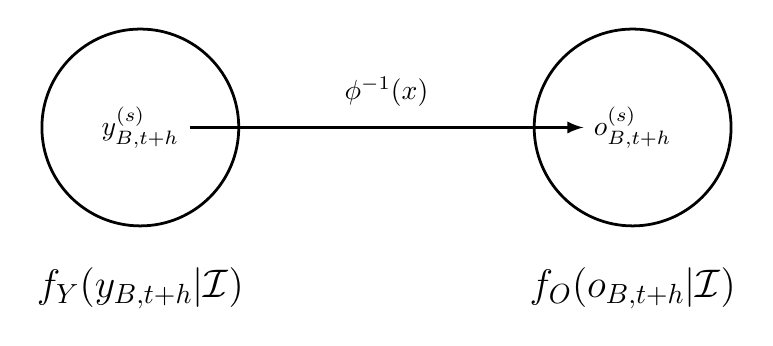
\begin{tikzpicture}[line width=1pt,>=latex]
\sffamily
\node (a2) {$y^{(s)}_{B,t+h}$};

\node[right=5cm of a2] (b2) {$o^{(s)}_{B,t+h}$};

\node[shape=ellipse,draw,minimum size=2.5cm,fit={(a2)}] {};
\node[shape=ellipse,draw,minimum size=2.5cm,fit={(b2)}] {};

\node[below=1.25cm of a2,font=\Large\bfseries] {$f_Y(y_{B,t+h}|\mathcal{I})$};
\node[below=1.25cm of b2,font=\Large\bfseries] {$f_O(o_{B,t+h}|\mathcal{I})$};

\draw[->,black] (a2) -- node[label=above:$\phi^{-1}(x)$] {} (b2);
\end{tikzpicture}
\end{figure}

On the original $(0,1)$-interval, we evaluate traffic occupancy forecasts for all full models $\mathcal{M}$ and final models $\mathcal{M}^*$. Monte Carlo methods are utilized to form the posterior predictive distribution  $f_O(o_{B,t+h}|\mathcal{I})$ to obtain point estimates from posterior means and credible regions from posterior quantiles. The last week of April 2000 was intentionally neglected for forecast evaluation. For each $(D,h)$-specific model, we have $n_h=480-h$ time points requiring forecasts. Forecasts for this week are obtained under the assumption that the posterior distribution of $\bm{\theta}_\mathcal{M}$ given the data $\mathcal{I}$ is static throughout the evaluation period. Typically, $f(\bm{\theta}_\mathcal{M}|\mathcal{I})$ can be updated when new information is added to $\mathcal{I}$.

Define $\mathbb{M}=\{L_1(D,h), R_1(D,h), L_2(D,h), R_2(D,h)\}$ to be the set of all full models and $\mathbb{M}^*=\{L^*_1(D,h), R^*_1(D,h), L^*_2(D,h), R^*_2(D,h)\}$ to be the corresponding reduced models. Given day $D$ and horizon $h$, we use three forecast accuracy metrics to answer the following quesions about $\mathbb{M}$ and $\mathbb{M}^*$:    
\begin{itemize}
   \item How do the models compare to each other?
   \item How do the full models compare to the final models?
   \item How do the models compare to benchmark naive and seasonal models?
 \end{itemize}

RMSFE can help answer the first two proposed questions. RMSFE allows the practitioner to understand traffic occupancy forecast error on the original percentage scale. Since RMSFE was used in the selection of $\mathcal{M}^*$,  we continue to apply RMSFE in model evaluation. The formula for RMSFE in terms of traffic occupancy is restated in \ref{eq:rmsfe2}.
\begin{equation}
 	\label{eq:rmsfe2}
  RMSFE(h)=\sqrt{\frac{1}{n_h}\sum\limits_{t=h+1}^{480} (O_{B,t}-\widehat{O}_{B,t})^2}
\end{equation}

Denote the mean absolute error (MAE) from daily baseline models $\mathcal{W}(D,h)$ and $\mathcal{S}_B(D)$ as $\textrm{MAE}_{W}(h)$ and $\textrm{MAE}_{S}$. Relative adaptations of MAE summarize the advantages of using a complex model over a simple benchmark choice \citep{Hyndman2006}. \cite{Theil1966} introduced this concept to random walks for evaluation of 1-step ahead performance. The $h$-specific relative MAFE (RelMAFE(h)) in Equation \ref{eq:relmafe} quantifies the benefit of a $(D,h)$-specific model to a $h$-specific random walk. We further this idea to the seasonal RelMAFE (SRelMAFE) in Equation \ref{eq:srelmafe} to understand advantages over seasonal profiles \citep{Makridakis2008}.
\begin{equation}
\label{eq:relmafe}
  RelMAFE(h)=\frac{1}{n_h}\sum\limits_{t=h+1}^{480}\left|\frac{O_{B,t}-\widehat{O}_{B,t}}{\textrm{MAE}_{W}(h)}\right|
\end{equation}
\begin{equation}
\label{eq:srelmafe}
  SRelMAFE(h)=\frac{1}{n_h}\sum\limits_{t=h+1}^{480}\left|\frac{O_{B,t}-\widehat{O}_{B,t}}{\textrm{MAE}_{S}}\right|
\end{equation}




\chapter{REGULARIZATION METHODS FOR SUBSET ARMA SELECTION}
\label{chap:co2}

\section{Introduction}

Let $\{y_t: t=1,2,\cdots,T\}$ be a sequentially observed discrete and equally-spaced sample from a weakly stationary, homoskedastic process $\{Y_t:t=\cdots,-1,0,1,\cdots\}$. For the purpose of forecasting future realizations i.e. $\hat{y}_{T+h}$ where $h\in\mathbb{N}$, we estimate a model of the general form $$y_{t}=f(y_{t-1},y_{t-2},\cdots,y_{t-p},\epsilon_{t-1},\epsilon_{t-2},\cdots,\epsilon_{t-q})+\epsilon_t.$$ Under homoskedasticity, $\{\epsilon_t\}$ is assumed to be white noise with mean 0 and variance $\sigma^2$.  Finite order parameters $p,q\in\mathbb{N}$ quantify the strength that past information has on prediction. Define $m=\max\{p,q\}$. In most cases, $m$ is small relative to $T$; however, when cyclical phenomenon is detected, $m\geq s$ where $s$ is the seasonal periodicity. The latter scenario leads to long gaps in relevant information for forecasting.

The seasonal autoregressive moving average (SARMA) process, popularized by \cite{Box1976}, jointly models the temporal short-term and seasonal dynamics of $\{y_t\}$ to forecast future unknown realizations. Let $B$ represent the backshift operator  where $B^ky_{t}=y_{t-k}$ and define polynomial functions $\Phi(B^s)=1-\sum\limits_{J=1}^P \Phi_J B^{sJ}$, $\phi(B)=1-\sum\limits_{j=1}^p \phi_j B^{j}$, $\Theta(B^s)=1+\sum\limits_{K=1}^Q \Theta_K B^{sK}$, and $\theta(B)=1+\sum\limits_{k=1}^q \theta_k B^{K}$. If the seasonal periodicity $s>1$ is known, the SARMA$(p,q)\times(P,Q)_{s}$ process in Equation \ref{eq:sarma} represents a viable family of models for forecasting.
\begin{equation}
\label{eq:sarma}
\Phi(B^s)\phi(B)y_t=\Theta(B^s)\theta(B)\epsilon_t
\end{equation}

The seasonal periodicity $s$ is typically unknown \textit{a priori}. Any SARMA model from Equation \ref{eq:sarma} algebraically reduces to an ARMA$(p^*,q^*)$ process $\phi^*(B)y_t=\theta^*(B)\epsilon_t$ where $\max\{p^*,q^*\}=\max\{Ps+p,Qs+q\} \textrm{ where } [p,P,q,Q,s]'\in\mathbbm{N}^5$. For example, consider a quarterly SARMA$(1,0)\times(1,0)_{4}$ process $\{x_t\}$ where $\phi_1=0.6$ and $\Phi_1=0.3$. The temporal dynamics of $\{x_t\}$ are equivalently modeled using an ARMA$(5,0)$ process such that $\bm{\phi}=[\phi_1,\phi_2,\phi_3,\phi_4,\phi_5]'=[0.6,0,0,0.3,-0.18]'$ (see Equation \ref{eq:sarma2arma}).
\begin{equation}
\label{eq:sarma2arma}
\begin{split}
\Phi(B^4)\phi(B)x_t&=\epsilon_t\\
(1-0.3B^4)(1-0.6B)x_t&=\epsilon_t\\
(1-0.6B-0.3B^4+0.18B^5)x_t&=\epsilon_t\\
\end{split}
\end{equation}

Fitting an ARMA$(p^*,q^*)$ model to an arbitrary series $\{y_t\}$ requires estimation of AR coefficients $\bm{\phi}=[\phi_1,\cdots,\phi_{p*}]'$ and MA coefficients $\bm{\theta}=[\theta_1,\cdots,\theta_{q^*}]'$. We desire estimates $\hat{\bm{\phi} }$ and $\hat{\bm{\theta} }$ that validate stationary and invertible regulatory assumptions. Stationarity and invertibility require all roots of both characteristic equations, $1-\phi_1z-\phi_2z^2-\cdots -\phi_{p^*}z^{p^*}=0$ and $1+\theta_1z+\theta_2z^2+\cdots +\theta_{q^*}z^{q^*}=0$, to be outside the unit circle. Classically, parameter estimation is conducted via method of moments, least squares, or maximum likelihood \citep{Hamilton1994, Cryer2008}. When $q^*=0$, these approaches are simple extensions of linear regression where the set of predictor variables are lagged realizations of the time series. If $q^*>0$, a linear model representation exists, but the presence of MA terms poses an estimation problem since the innovations $\{\epsilon_t\}$ are unobservable and dependent on $\bm{\phi}$ and $\bm{\theta}$. Popular least squares and maximum likelihood estimation methods become far less efficient and require nonlinear optimization techniques.

Any ARMA$(p^*,q^*)$ model that satisfies the invertibility condition has an $AR(\infty)$ representation, i.e. $(1-\sum\limits_{j=1}^\infty \phi^\prime_jB^j)y_t=\epsilon_t$. If we know $\bm{\phi}^\prime$, we can obtain the full set $\{\epsilon_t\}$. The residuals $\{\hat{\epsilon}_t: t=\tilde{p}+1,\cdots,T\}$ of a long AR$(p^\prime)$ process fitted to  $\{y_t\}$ can approximate the unobserved $\{\epsilon_t\}$.  This approach was initially proposed by \cite{Hannan1982} to obtain quick estimation of ARMA$(p^*,q^*)$ as it avoids previously mentioned estimation issues. For further information, see \citet[pp. 156-158]{Brockwell2016}.

The model orders $p^*$ and $q^*$ can be heuristically selected through inspection of sample autocorrelation and partial autocorrelation functions (abbreviated ACF and PACF, respectively). This non-scientific approach could lead to misspecified models and possibly poor forecasting performance. Suppose $p$ and $q$ are safe upper bounds such that $p\geq p^*$ and $q\geq q^*$. For the $(p+1)(q+1)$ different ARMA models, final order selection can be based off minimization of some measure of prediction error (PE). Information criteria such as AIC \citep{Akaike1974} or BIC \citep{Schwarz1978} are popular metrics that penalize for model complexity. Stepwise selection algorithms are usually instituted to accelerate this process.

These approaches are best suited for estimating ARMA processes where $\phi_j\neq 0$ and $\theta_k \neq 0$ for $j\in\{1,\cdots,p^*\}$ and $k\in\{1,\cdots,q^*\}$. For the scenario in Equation \ref{eq:sarma2arma}, correct identification of $p^*=5$ and $q^*=0$ still leads to overfitting since truly zero parameters, $\phi_2$ and $\phi_3$, are included in estimation. We define the true process in Equation \ref{eq:sarma2arma} as a subset ARMA$(5,0)$ model where $\bm{\phi}=[\phi_1,\phi_4,\phi_5]'=[0.6,0.3,-0.18]'$. Common approaches for ARMA$(p,q)$ model selection become less efficient and reliable when searching through the $2^{(p+q)}$ unique subset ARMA$(p,q)$ models.	

Let $\bm{y}=[y_{m},\cdots,y_T]'$, $\bm{\epsilon}=[\epsilon_{m},\cdots,\epsilon_T]'$, $\bm{\beta}=[\bm{\phi}',\bm{\theta}']'=[\phi_1,\cdots,\phi_p,\theta_1,\cdots,\theta_q]'$, and 
\begin{equation*}
\bm{X}=\begin{bmatrix} \bm{x}'_{m}  \\
					\bm{x}'_{m+1}  \\
					\vdots \\
					\bm{x}'_{T} \\
	\end{bmatrix} =
	\begin{bmatrix} y_{m-1} & \cdots & y_{m-p} &
					\hat{\epsilon}_{m-1} & \cdots & \hat{\epsilon}_{m-q} \\
					y_{m} & \cdots & y_{m-p+1} &
					\hat{\epsilon}_{m} & \cdots & \hat{\epsilon}_{m-q+1} \\
					\vdots & \ddots & \vdots &\
					\vdots & \ddots & \vdots & \\
					y_{T-1} & \cdots & y_{T-p} &
					\hat{\epsilon}_{T-1} & \cdots & \hat{\epsilon}_{T-q} \\
	\end{bmatrix}.
\end{equation*}
The ARMA$(p,q)$ model is equivalently represented by $\bm{y}=\bm{X}\bm{\beta}+\bm{\epsilon}$. Recall that $\hat{\epsilon}_t$ are residuals from fitted AR$(p^\prime)$ models used to estimate unknown innovations. Similar to estimation via conditional least squares and conditional maximum likelihood \citep{Hamilton1994}, the first $m-1$ observations are lost in parameter estimation where $m=p^\prime+max\{p,q\}+1$. For reduction of $m$, selection of $p^\prime$ can be based off AIC or BIC  \citep{Hannan1984a,Chen2011}. Also, it is important to note $\{y_t\}$ is assumed to be mean-centered. An additional mean parameter $\mu$ can be included in $\bm{\beta}$ via  binding a column of $1$s to $\bm{X}$.

Presenting the ARMA$(p,q)$ model as a linear Gaussian model is quite advantageous. For both linear and generalized linear models, the least absolute shrinkage and selection operator (LASSO) of \cite{Tibshirani1996} efficiently combines model selection and estimation. The LASSO estimator in Equation \ref{eq:lasso2} achieves sparsity through $\ell_1$ penalization of the least squares criterion.  The tuning parameter $\lambda >0$ controls overall shrinkage of $\bm{\beta}$ towards 0. Consequentially, the LASSO estimate is a function of $\lambda$, but full solution paths are quickly obtained via well-developed algorithms \citep{Efron2004}. The optimal $\lambda$ is often based off minimization of AIC, BIC, or some generalization of prediction error. The effectiveness of LASSO motivated analogous Bayesian approaches using Laplace priors \citep{Park2008, Yuan2005}. Similarly, hyperpriors placed on $\lambda$ encourage data-driven shrinkage of posterior estimates.
\begin{equation}
\label{eq:lasso2}
\hat{\bm{\beta}}_{L} (\lambda)= \underset{\bm{\beta}}{\textrm{argmin }}  ||\bm{y}-\bm{X}\bm{\beta}||^2 + \lambda \sum\limits_{i=1}^{p+q}|\beta_i|
\end{equation}

Applying LASSO in time series analysis is potentially problematic since the ARMA model matrix $\bm{X}$ contains correlated predictors.  \cite{Nardi2011} explored the consistency properties of $\hat{\bm{\beta}}_{L}$ for AR$(p)$ processes to approximate realizations from ARMA data generating processes (DGPs). However, high correlation between non-zero and irrelevant ARMA predictors may violate the ``irrepresentable condition" required for sign and model selection consistency \citep{Zhao2006}. \cite{Hebiri2013} demonstrate that highly collinear designs yield underestimation of $\lambda$ and poor prediction. Modified LASSO and other methods with better asymptotic properties mitigate the consequences of correlated predictors.

In our context, $p$ and $q$ should be safely overestimated, resulting in a sparse parameter vector $\bm{\beta}$. In this article, we explore the application of regularization methods to automate subset ARMA$(p,q)$ selection and estimation of $\bm{\beta}$. Section \ref{sec:methods} presents three different methods that incorporate subset selection through regularization estimation. The first two methods extend off work from \cite{Chen2011}. A discussion of cross-validation techniques explores alternative ways to select regularization tuning parameters. The final regularization method is developed under the Bayesian framework for a contrast to the preceding classical approaches. Section \ref{sec:mc} contains simulation studies evaluating and comparing the different methods. Section \ref{sec:co2app} applies the methods to monthly carbon dioxide time series collected from two atmospheric observatories.










\section{Methods}
\label{sec:methods}

Assume $y_t$ follows a subset ARMA$(p,q)$ process. Recall the matrix ARMA representation $\bm{y}=\bm{X}\bm{\beta}+\bm{\epsilon}$ where $\bm{\beta}=[\bm{\phi}',\bm{\theta}']=[\beta_1,\cdots,\beta_{p+q}]'$. The set $\mathcal{V}=\{i:\beta_i\neq 0\}$ indicates the AR and MA terms relevant to the true process. If the cardinality $|\mathcal{V}|<p+q$, irrelevant predictors are included in the ARMA model matrix $\bm{X}$. Given observed data $\{y_t: t=m,m+1,\cdots,T\}$, we obtain estimates $\hat{\bm{\beta}}$ for $\bm{\beta}$ and $\hat{\mathcal{V}}=\{i:\hat{\beta}_i\neq 0\}$ for $\mathcal{V}$. Multiple researchers have theoretically explored the asymptotic behavior of penalized estimators including the popular oracle property \citep{Fan2001,Fan2004,Fan2011}. A method for estimating $\bm{\beta}$ is described as oracle if the estimator $\hat{\bm{\beta}}$ asymptotically behaves as an estimator developed under prior knowledge of $\mathcal{V}$. Under these considerations, we describe approaches to estimate ARMA coefficients while simultaneously identifying $\mathcal{V}$ through shrinking irrelevant effects to 0.

\subsection{Adaptive LASSO}

\cite{Zou2006} highlighted the conditional consistency of LASSO and introduced adaptive LASSO (ADLASSO) which enjoys the oracle properties. For a chosen $\eta>0$, we a define vector of weights $\hat{\bm{w}}=|\hat{\bm{\beta}}+1/T|^{-\eta}$ where $\hat{\bm{\beta}}$ represents an initial estimate of $\bm{\beta}$ derived using ordinary least squares (OLS), ridge, or LASSO regression. The additional $1/T$ exists so division by $0$ is prevented. The ADLASSO estimator $\hat{\bm{\beta}}_{AL}$ is described in Equation \ref{eq:adlasso2}. The tuning parameter $\lambda>0$ controls the degree of penalization across all ARMA terms while coefficient-specific weights fine tune shrinkage.
\begin{equation}
\label{eq:adlasso2}
\hat{\bm{\beta}}_{AL} (\lambda)= \underset{\bm{\beta}}{\textrm{argmin }}  ||\bm{y}-\bm{X}\bm{\beta}||^2 + \lambda \sum\limits_{i=1}^{p+q} \hat{w}_{i}|\beta_i|
\end{equation}

For subset ARMA model selection, \cite{Chen2011} showed ADLASSO is an oracle procedure under 3 regulatory assumptions when $\hat{\bm{\beta}}=(\bm{X}'\bm{X})^{-1}\bm{X}'\bm{y}$. Proof of this result followed from using a long AR$(p^\prime)$ process to estimate unknown innovations. Simulation results indicated best empirical performance when the initial estimate $\hat{\bm{\beta}}=\hat{\bm{\beta}}_L$. Following from \cite{Zou2006} and \cite{Chen2011}, we fix $\eta=2$ and only consider $\hat{\bm{\beta}}_L$ in the formulation of $\hat{\bm{w}}$.

\subsection{Adaptive Elastic Net}
The ADLASSO procedure has become popular in time series analysis since parsimonious models typically improve forecasting. Incorporating lags of exogenous time series in $\bm{X}$ adds complexity that ADLASSO can discriminate against. Assuming information becomes less relevant for forecasting as time passes has encouraged modifications for more complicated full models. For example, lag lengths can be included in the functional representation of $\hat{\bm{w}}$ to further encourage penalization for long-lagged terms \citep{Park2013,Konzen2016}. When seasonal effects are prevalent, these ADLASSO modifications may completely eliminate important terms at long lags. In this section, we digress from ADLASSO without just redefining the weights.

The elastic net (ENET) of \cite{Zou2005} has applicability in this context where $\bm{X}$ contains two groups of predictors with potentially high pairwise collinearity. Although variable selection benefits of LASSO would be lost, the ridge estimator of \cite{Hoerl1970} could lead to better forecasting. The ENET estimator in Equation \ref{eq:enet}  introduces another tuning parameter $\alpha\in[0,1]$ to influence the trade-off between $\ell_1$ and $\ell_2$ penalties \citep{DeMol2009}. The original motivation of ENET was to overcome model selection limitations of LASSO when the number of parameters is larger than the sample size, a common problem in bioinformatic data \citep{Zou2005}. This problem is not prevalent in time series analysis; however, seasonal dynamics, which require multiple cycles to estimate, are difficult to identify when data is limited and/or the period is large. Hypothetically, it makes sense to evaluate empirical performance of ENET in this context.
\begin{equation}
\label{eq:enet}
\hat{\bm{\beta}}_{E} (\lambda,\alpha)= \underset{\bm{\beta}}{\textrm{argmin }}  ||\bm{y}-\bm{X}\bm{\beta}||^2 + \lambda\bigg[ (1-\alpha) \sum\limits_{i=1}^{p+q} \beta^2_i+ \alpha\sum\limits_{i=1}^{p+q} |\beta_i| \bigg]
\end{equation}

As we have seen, ADLASSO satisfies the oracle properties \citep{Zou2006} and ENET \citep{Zou2005} manages collinearity. \cite{Zou2009a} exploit both advantages by modifying the $\ell_1$ penalty Equation \ref{eq:enet} to match the weighted form in Equation \ref{eq:adlasso2}. This adaptive ENET (ADENET) estimator is formally presented in Equation \ref{eq:aenet}. \cite{Zou2009a} recommend selecting $\hat{\bm{\beta}}=\hat{\bm{\beta}}_{E}$. Since $\hat{\bm{\beta}}_{E}$ depends on the choice of two tuning parameters, $\lambda$ and $\alpha$, optimal selection requires a grid search. Upon empirical evaluation, setting $\hat{\bm{\beta}}=\hat{\bm{\beta}}_{L}$ is sufficient for obtaining the initial weights.
\begin{equation}
\label{eq:aenet}
\hat{\bm{\beta}}_{AE} (\lambda,\alpha)= \underset{\bm{\beta}}{\textrm{argmin }}  ||\bm{y}-\bm{X}\bm{\beta}||^2 + \lambda\bigg[ (1-\alpha)  \sum\limits_{i=1}^{p+q} \beta^2_i+ \alpha\sum\limits_{i=1}^{p+q} \hat{w}_{i}|\beta_i| \bigg]
\end{equation}


\subsection{Options for Selecting Tuning Parameters}
The adaptive estimators $\hat{\bm{\beta}}_{AL} (\lambda)$ and $\hat{\bm{\beta}}_{AE} (\lambda,\alpha)$ depend on choices for $\lambda$ and $\alpha$. Given finite sets $\mathcal{L}=\{\lambda_j>0: j=1,\cdots,J\}$ and $\mathcal{A}=\{0<\alpha_k<1: k=1,\cdots,K\}$, full solution paths for both estimators can be produced via LARS algorithm \citep{Efron2004} or coordinate descent \citep{glmnet}. Essentially, each $\lambda\in\mathcal{L}$ and $\alpha\in\mathcal{A}$ corresponds to a different subset ARMA$(p,q)$ model, equating to $|\mathcal{L}|$ different ADLASSO models and $|\mathcal{L}|\times|\mathcal{A}|$ different ADENET models. The optimal $\lambda^*$ and $\alpha^*$ should be empirically chosen based off some estimate of forecasting performance. In this section, we explore different algorithms to select final subset ARMA models, $\hat{\bm{\beta}}_{AL}=\hat{\bm{\beta}}_{AL}(\lambda^*)$ and $\hat{\bm{\beta}}_{AE}=\hat{\bm{\beta}}_{AE}(\lambda^*,\alpha^*)$. See \citet[pp. 241-254]{Hastie2009a} for classic approaches to select tuning parameters.

\subsubsection{SELECTION BASED ON AIC OR BIC}

Popular information criteria AIC and BIC can be used to select tuning parameters $\lambda$ and $\alpha$. We consider the effect of using these penalized measures of error in model selection for the initial LASSO-based weights $\hat{\bm{w}}$ and final models. To quantify model complexity, consider the approximate degrees of freedom $\hat{v}(\lambda)$=$|\widehat{\mathcal{V}}(\lambda)|$ where $\widehat{\mathcal{V}}(\lambda)=\{i:\hat{\beta}_i\neq 0\}$ \citep{Zou2007}. The AIC and BIC formulas for LASSO and ADLASSO are given in Equation \ref{eq:aicbic}. For ENET and ADENET, $\hat{\bm{\beta}}(\lambda)$ and $\hat{v}(\lambda)$ must be replaced with $\hat{\bm{\beta}}(\lambda,\alpha)$ and $\hat{v}(\lambda,\alpha)$.
\begin{equation}
\label{eq:aicbic}
\begin{split}
\textrm{AIC}(\hat{\bm{\beta}}(\lambda))&=2\hat{v}(\lambda)+(T-m+1)\log\bigg(\frac{||\bm{y}-\bm{X}\hat{\bm{\beta}}(\lambda)||^2}{T-m+1}\bigg)\\
\textrm{BIC}(\hat{\bm{\beta}}(\lambda))&=\log(T-m+1)\hat{v}(\lambda)+(T-m+1)\log\bigg(\frac{||\bm{y}-\bm{X}\hat{\bm{\beta}}(\lambda)||^2}{T-m+1}\bigg)\\
\end{split}
\end{equation}

Choice of information criteria (BIC or AIC) is not a Bayesian versus non-Bayesian argument, but an argument about whether true models exist and can be discovered \citep{burnham2003}. Empirical analysis indicates AIC more frequently outperforms in prediction, but BIC's stronger penalty notoriously leads to better model selection \citep{Burnham2004}. The true complexity of the unknown DGP and the path of AIC/BIC influence this decision\citep{Shao1997,burnham2003}. \cite{Chen2011} consider AIC and BIC in both stages of ADLASSO and acknowledge this phenomenon in simulation of subset ARMA models.  Averaged models weighted based off AIC and BIC are often superior in prediction to individual models, but this is out of the scope of this paper \citep{Burnham2004}. 

Philosophical differences aside, we evaluate both measures in model selection and forecasting. ADLASSO and ADENET are two stage procedures. In \cite{Chen2011}, only BIC is used for LASSO estimated weights. These weights are crucial in the overall effectiveness of both estimation algorithm. If the BIC penalty overshrinks estimates toward $0$, relevant parameters can be unrecognized in the second stage regardless of whether AIC or BIC are used. We favor AIC in the first stage providing safer protection against losing too many key variables. To provide comparison to \cite{Chen2011}, we consider three of four possible combinations: AIC in both stages, AIC then BIC, and BIC in both stages. The last option was evaluated in \cite{Chen2011}.

\subsubsection{Selection Based on Cross-Validation}

Optimal tuning parameters for regularization are typically chosen via cross-validation (CV) \citep{Hastie2009a}. This approach has been popular for model selection in classic linear regression since \cite{Stone1974}. For $K$-Fold CV (CV-K), we begin by splitting the usable $T-m+1$ portion of the time series into $K$ separate folds. Each fold acts as a testing period for models fitted to remaining data. Figure \ref{fig:kcvplots} illustrates this partitioning for CV-5 and CV-10 assuming $T-m+1=100$. Random assignment of data to $K$ folds leads to approximately $100/K$ prediction points in each data split.
\begin{figure}[htbp!]
	\caption{General $K$-fold Cross-Validation for Model Selection for $K=5$ (top) and $K=10$ (bottom)}
	\center
	\label{fig:kcvplots}
	\includegraphics[scale=0.58]{kcvplots}
\end{figure}

Following similar notation from \cite{Hastie2009a}, $\kappa:\{m,m+1,\cdots,T\}\to\{1,\cdots,K\}$ is the indexing function mapping data to specific testing groups. An estimate of PE is obtained for each $\lambda \in \mathcal{L}$ and $\alpha \in \mathcal{A}$, and optimal tuning parameters are chosen based on minimization of this estimate. Specifically for the LASSO cases, $\widehat{\textrm{PE}}(\lambda)$ is expressed in Equation \ref{eq:lassocvpe}. We use $\hat{\bm{\beta}}_{\kappa(t)}(\lambda)$ to represent the estimated ARMA parameters from models fitted to data not in the $\kappa(t)$ group. The most exhaustive case is leave-one-out CV (LOOCV) where $K=(T-m+1)$ and  $\kappa(t)=t-m+1$. Obtaining $\widehat{\textrm{PE}}(\lambda)$ for LOOCV would be time consuming if not for the generalized CV (GCV) of \cite{Wahba1978}.
\begin{equation}
\label{eq:lassocvpe}
	\widehat{\textrm{PE}}(\lambda)=\frac{1}{T-m+1}\sum\limits_{t=m}^T \bigg(y_t-\bm{x}_t'\hat{\bm{\beta}}_{\kappa(t)}(\lambda)\bigg)^2
\end{equation}


\subsubsection{Selection Based on Out-of-Sample EvaluationSELECTION BASED ON OUT-OF-SAMPLE EVALUATION}

Applied statisticians prefer CV-K or LOOCV when data is cross-sectional. This approach is not intuitive for time series data where prediction on a randomly selected subset of the full data does not seem like forecasting. For a particular $\tau\in (0,1)$, the out-of-sample (OOS) method estimates $\hat{\bm{\beta}}(\lambda)$ from the first $(1-\tau)\times 100\%$ of the data (TRAIN) and forecasts on the final $\tau\times 100\%$ (TEST). Equation 
\ref{eq:lassooos} equates to mean squared forecast error (MSFE) and is used to optimally select tuning parameters. 
\begin{equation}
\label{eq:lassooos}
	\widehat{\textrm{PE}}(\lambda)=\frac{1}{\tau T}\sum\limits_{t\in \textrm{TEST}} \bigg(y_t-\bm{x}_t'\hat{\bm{\beta}}(\lambda)\bigg)^2
\end{equation}

For subset ARMA selection, order parameters $p$ and $q$ are fixed and quantify the memory required to forecast.  In our naive description of OOS, we ignore the fact that some of our forecasts in the TEST period are obtained using data in the TRAIN period. Given $p$ and $q$, the final $d=\max\{p,q\}$ points in the TRAIN period are ignored in model fitting. Now, models are strictly evaluated on future data independent of the TRAIN period. In some literature, this is default OOS \citep{Bergmeir2018}; however, we abbreviate this modified version depOOS to highlight the additional considerations being made. Figure \ref{fig:oosplots} displays the difference data division between OOS and depOOS.

\begin{figure}[htbp!]
	\caption{Variations of Out-of-Sample Procedures for Model Selection}
	\center
	\label{fig:oosplots}
	\includegraphics[scale=0.58]{oosplots}
\end{figure}


\subsubsection{Selection Based on Blocked CV}
Classic CV estimates the expected PE constructed from predictions on unfitted data. This may lead to a poor estimate for time series data where the popular ``independent observation" assumption is violated \citep{Arlot2010}. \cite{Burman1994} modified LOOCV by ignoring the $d$ observations before and after each time point in fitting. Similarly, \cite{Bergmeir2018} describe and evaluate a non-dependent version CV-K. For $T-m+1=100$ and $d=4$, we show this modification in Figure \ref{fig:depkcvplots} which is based off the same random assignment in Figure \ref{fig:oosplots}. Controlling the number of points available for fitting models is difficult for this modified CV-K even for a low order $d$. This along with the poor empirical results in \cite{Bergmeir2018} removes this approach from consideration.

\begin{figure}[htbp!]
	\caption{Non-Dependent $K$-fold Cross-Validation for Model Selection for $K=5$ (top) and $K=10$ (bottom)}
	\center
	\label{fig:depkcvplots}
	\includegraphics[scale=0.58]{depkcvplots}
\end{figure}

In this paper, we propose blocked variants of CV that retain the ordered structure and ensure reasonable sample sizes for model fitting. \cite{Racine2000} alters the CV method of \cite{Burman1994} to measure prediction error on blocks of data around each data point for each fold. \cite{Bergmeir2012} proposes K-fold blocked CV (BCV-K) where naturally ordered data is evenly split into $K$ sets.  For order $d$, the first and last $\lceil \frac{d}{2} \rceil$ data points are removed from each block to remove dependence, and ordinary CV is performed using the blocks. See Figure \ref{fig:bcvplots} for for BCV-5 and BCV-10 when $d=4$. 

\begin{figure}[htbp!]
	\caption{Non-Dependent $K$-Block Cross-Validation for Model Selection for $K=5$ (top) and $K=10$ (bottom)}
	\center
	\label{fig:bcvplots}
	\includegraphics[scale=0.58]{bcvplots}
\end{figure}

Analogous to LOOCV, we extend BCV-K to leave-one-block-out design (LOBOCV). This approach is similar to $\textrm{BCV-K}^*$ when $K^*=\lfloor \frac{T-m+1}{d} \rfloor$ since we divide time series sequentially into $K^*$ blocks. Block specific estimates $\widehat{\textrm{PE}}_K(\lambda)$ or $\widehat{\textrm{PE}}_K(\lambda,\alpha)$ are evaluated after models are fitted to data in non-adjacent blocks. In LASSO cases, overall BCV prediction error is based on expression in Equation \ref{eq:lobocv2}. Similar expressions are seen for BCV-5 and BCV-10 since all prediction periods are of the same length. This is a key difference to the initial proposed non-dependent CV-K.
\begin{equation}
\label{eq:lobocv2}
	\widehat{\textrm{PE}}(\lambda)=\frac{1}{K}\sum\limits_{k=1}^K \widehat{\textrm{PE}}_K(\lambda)
\end{equation}

\begin{figure}[htbp!]
	\caption{Leave-One-Block-Out Cross-Validation for Model Selection}
	\center
	\label{fig:lobocvplots}
	\includegraphics[scale=0.58]{lobocvplots}
\end{figure}

Literature evaluates these methods on the error between estimated $\widehat{\textrm{PE}}$ using CV and OOS and true $\textrm{PE}$ from data completely ignored \citep{Bergmeir2014,Bergmeir2018}. Typical experiments examine this error when the fitted models are known to be misspecified \citep{Burman1994,Racine2000,Bergmeir2018}. These discussions are not the focus of this paper. We only explore the performance of these methods in selection of $\lambda$ and $\alpha$ for ADLASSO and ADENET. 

\subsection{Bayesian Predictive Posterior Projection Method}
\subsubsection{Traditional Bayesian Model Selection}
Classic Bayesian model selection starts by reparamaterizing $\beta_i^*=\xi_i\beta_i$ where $\xi_i\in\{0,1\}$. For the new vector of parameters $\bm{\beta}^*=[\beta^*_1,\beta^*_2,\cdots,\beta^*_{p+q}]'$, the set of relevant parameters $\mathcal{V}=\{i:\beta^*_i\neq 0\}=\{i:\xi_i\neq 0\}$. Let $\mathcal{N}_p(\bm{\mu},\sigma^2\bm{\Sigma}_p)$ represent the $p$-dimensional multivariate normal distribution and $BERN(\pi)$ represent the $Bernouilli$ distribution. If dimension $p$ is not given, assume $p=1$. The scenario $\bm{\Sigma}_p=\bm{I}_p$, where $\bm{I}_p$ is $p\times p$ identity matrix, implies that $\beta_j\perp\beta_k$ for all $j\neq k$. For the new linear model  $\bm{y}=\bm{X}\bm{\beta}^*$, \cite{Kuo1998} suggested the prior $p(\beta_i,\xi_i)=p(\beta_i)p(\xi_i)$ indicating $\beta_i \perp \xi_i$. Later authors suggested $p(\beta_i,\xi_i)=p(\beta_i|\xi_i)p(\xi_i)$ where $p(\beta_i|\xi_i)=(1-\xi_i)p(\beta_i|\xi_i=1)+\xi_i p(\beta_i|\xi_i=0) $ is a mixture prior \citep{Carlin1995}. The popular ``spike and slab" prior is of this type where the slab $p(\beta_i|\xi_i=1)$ is uninformative and the spike $p(\beta_i|\xi_i=0)$ is concentrated around 0 \citep{Mitchell1988,George1993, Carlin1995}. Common to all methods, $\xi_i \sim BERN(\pi_{i,0})$ where $\pi_{i,0}$ is the prior probability that variable $\beta_i \neq 0$. All subset models are equally likely \textit{a priori} when $\pi_{i,0}=0.5$. Sampling from $p(\bm{\beta},\bm{\xi},\sigma^2|\bm{y},\bm{X})$ requires a combination of approaches \citep{Dellaportas2002}, and the posterior mode of $\bm{\xi}$ indicates the best model. Posterior model probabilities and Bayes factors are used to discriminate between possible sub models. Implementation of Bayesian model averaging is within this umbrella \citep{Raftery1997,Hoeting1998,Hoeting1999}.

\subsubsection{Bayesian Regularization}
Posterior samplers based on 2-component mixture priors are often slow in exploring high-dimensional spaces. Priors developed from continuous mixing densities achieve similar results without requiring tuning. For example, \cite{Andrews1974} presented a hierarchy for the $Laplace$ (i.e. $Double-Exponential$) distribution from scale-mixture of $Normals$ using $Exponential$ mixing density. The Bayesian LASSO \citep{Park2008,Hans2009} uses this hierarchy for $p(\bm{\beta}|\sigma^2)$ understanding the link between $\ell_1$-regularization and posterior modes from $Laplace$ priors \citep{Tibshirani1996}. See \cite{OHara2009} for a historical look and comparison of adaptive Laplacian priors to discontinuous mixture priors.

Since the introduction of Bayesian LASSO, research in Bayesian regularization methods has exploded over the last ten years. Bayesian methods analogous to ADLASSO \citep{Leng2014}, ENET \citep{Li2010a}, and ADENET \citep{Stankiewicz2015} have been introduced and applied. The prior hierarchies of the aforementioned methods are in a class of ``global-local" shrinkage priors \citep{Polson2010}. The recently popular Bayesian horseshoe (BHS) prior falls in this class where $half-Cauchy$ priors are used to enforce global sparsity while preventing overshrinking of relevant parameters \citep{Carvalho2009,Carvalho2010}. The BHS enjoys the important oracle properties established for ADLASSO and ADENET \citep{Datta2015}. \cite{Bhadra2016} introduced horseshoe+ ($\textrm{BHS}^+$) which includes an additional layer of local shrinkage improving estimation when $\bm{\beta}$ is ``ultra-sparse". In subset ARMA selection, we safely choose $p$ and $q$ large enough to ensure any long lag seasonal effects may be discovered. Overestimation of $p$ and $q$ may introduce many non-seasonal ARMA terms that are equal to 0.  For these reasons, we utilize BHS and $\textrm{BHS}^+$ type priors for $\beta_i$. 

The hierarchical representations of BHS and $\textrm{BHS}^+$ displayed in Equations \ref{eq:makschmidths} \& \ref{eq:makschmidthsp} allow posterior sampling via Gibbs \citep{Makalic2016b}. These hierarchies developed from understanding that $\tau^2|\xi \sim \mathcal{IG}(1/2,1/\xi)$ and $\xi\sim\mathcal{IG}(1/2,1/a)$ imply $\tau\sim\mathcal{C}^+(0,a)$ \citep{Wand2011}. Expressions $\mathcal{IG}(a,b)$ and $\mathcal{C}^+(0,a)$ represent $Inverse-Gamma$ and $half-Cauchy$ distributions, respectively. The latent parameter $\tau$ controls overall regularization. Global shrinkage parameter $\tau$ can be fixed \citep{vanderPas2014}, updated via empirical Bayes \citep{Johnstone2004}, or given a hyperprior \citep{Carvalho2009,Carvalho2010}. Prior beliefs on the degree of sparsity in $\bm{\beta}$  should drive the handling of $\tau$ improving regularization \citep{vanderPas2014,Piironen2016}. The additional latent parameters $\lambda_i$ fine tune the regularization induced by $\tau$ for individual $\beta_i$. Heavy-tails of $\mathcal{C}^+(0,1)$ prevent relevant ARMA parameters from being overshrunk to 0.
\begin{equation}
\label{eq:makschmidths}
\begin{split}
\bm{y}|\bm{X},\bm{\beta},\sigma^2 & \sim \mathcal{N}_{p+q}(\bm{X}\bm{\beta},\sigma^2\bm{I}_{p+q}) \\
\beta_i|\lambda^2_i,\tau^2,\sigma^2 & \sim \mathcal{N}(0,\lambda^2_i\tau^2\sigma^2) \\
\sigma^2 & \sim \sigma^{-2}\textrm{d}\sigma^2 \\
\lambda^2_i|\nu_i & \sim \mathcal{IG}(1/2,1/\nu_i)\\
\tau^2|\xi & \sim \mathcal{IG}(1/2,1/\xi)\\
\nu_1,\cdots, \nu_{p+q}& \sim \mathcal{IG}(1/2,1) \\
\xi & \sim \mathcal{IG}(1/2,1) \\
\end{split}
\end{equation}
\begin{equation}
\label{eq:makschmidthsp}
\begin{split}
\bm{y}|\bm{X},\bm{\beta},\sigma^2 & \sim \mathcal{N}_{p+q}(\bm{X}\bm{\beta},\sigma^2\bm{I}_{p+q}) \\
\beta_i|\lambda^2_{1,i},\lambda^2_{2,i},\tau^2,\sigma^2 & \sim \mathcal{N}(0,\lambda^2_{1,i}\lambda^2_{2,i}\tau^2\sigma^2) \\
\sigma^2 & \sim \sigma^{-2}\textrm{d}\sigma^2 \\
\lambda^2_{1,i}|\nu_{1,i} & \sim \mathcal{IG}(1/2,1/\nu_{1,i})\\
\lambda^2_{2,i}|\nu_{2,i} & \sim \mathcal{IG}(1/2,1/\nu_{2,i})\\
\tau^2|\xi & \sim \mathcal{IG}(1/2,1/\xi)\\
\nu_{1,i},\cdots, \nu_{1,p+q} & \sim \mathcal{IG}(1/2,1) \\
\nu_{2,i},\cdots, \nu_{2,p+q} & \sim \mathcal{IG}(1/2,1) \\
\xi & \sim \mathcal{IG}(1/2,1) \\
\end{split}
\end{equation}

\subsubsection{Predictive Posterior Projection}

Define $\mathcal{V}_F=\{1,2,\cdots,p+q\}$. For the fully saturated ARMA$(p,q)$ model, let $\hat{\bm{\beta}}_{HS}(\mathcal{V}_F)$ and $\hat{\bm{\beta}}_{HS^{+}}(\mathcal{V}_F)$ correspond to the posterior means of $\bm{\beta}$ under BHS and $\textrm{BHS}^+$, respectively. Both $\hat{\bm{\beta}}_{HS}(\mathcal{V}_F)$ and $\hat{\bm{\beta}}_{HS^{+}}(\mathcal{V}_F)$ are quality initial estimates of $\bm{\beta}$ but not sparse since $\hat{\beta}_i \neq 0$ for all $i$. Obtaining these estimates is analogous to the first stages of ADLASSO and ADENET. Any $\mathcal{V}_\perp \subset \mathcal{V}_F$ characterizes a particular subset ARMA$(p,q)$ model via indicating the parameters of $\bm{\beta}$ included.  Although the best model $\mathcal{V}^* \subset \mathcal{V}_F$ may differ under BHS and $\textrm{BHS}^+$, the corresponding final subset ARMA$(p,q)$ models are defined $\hat{\bm{\beta}}_{HS}=\hat{\bm{\beta}}_{HS}(\mathcal{V}^*)$ and $\hat{\bm{\beta}}_{HS^{+}}=\hat{\bm{\beta}}_{HS^{+}}(\mathcal{V}^*)$. In this section, we present a Bayesian inspired algorithm to select $\mathcal{V}^*$ after an initial BHS or $\textrm{BHS}^+$ estimation. For simplicity, we generalize an outline of this approach for both BHS and $\textrm{BHS}^+$.

After Bayesian estimation, the full model $\mathcal{V}_F$ represents a viable reference model. The sets $\{\bm{\beta}^{(s)}(\mathcal{V}_F)\}_{s=1}^S$ and $\{\sigma^{(s)}(\mathcal{V}_F)\}_{s=1}^S$ are the $S$ posterior samples under the reference model. Given a proposed nested model $\mathcal{V}_\perp \subset \mathcal{V}_F$, \cite{Goutis1998} suggested the Kullback-Leibler (K-L) distance \citep{Kullback1951} to evaluate discrepancy between $\mathcal{V}_F$ and $\mathcal{V}_\perp$. Classic model selection via AIC is based on K-L information and derivable from a Bayesian perspective \citep{Akaike1974,Akaike1985,burnham2003,Burnham2004}. For a future value $\tilde{y}=y_{T+1}$, the loss in explanatory power from using $\mathcal{V}_\perp$ instead of $\mathcal{V}_F$  is assessed by the K-L distance between posterior predictive distributions listed in Equation \ref{eq:projpreddist}. If the discrepancy between $p(\tilde{y}|\bm{y},\bm{X},V_F)$ and $p(\tilde{y}|\bm{y},\bm{X},V_\perp)$ is small, the more parsimonious $\mathcal{V}_\perp$ is favored.  The foundation of this concept is provided in \cite{Dupuis2003,Nott2010,vehtari2012,Piironen2015b,Piironen2017}.
\begin{equation}
\label{eq:projpreddist}
\begin{split}
p(\tilde{y}|\bm{y},\bm{X},V_F)&=\int\int p(\tilde{y}|\bm{y},\bm{X},\bm{\beta}_F,\sigma_\perp,V_F)p(\bm{\beta}_F,\sigma_F|\bm{y},\bm{X},V_F) \textrm{ d}\bm{\beta}_F \textrm{ d}\sigma_F\\
p(\tilde{y}|\bm{y},\bm{X},V_\perp)&=\int\int p(\tilde{y}|\bm{y},\bm{X},\bm{\beta}_\perp,\sigma_\perp,V_\perp)p(\bm{\beta}_\perp,\sigma_\perp|\bm{y},\bm{X},V_\perp) \textrm{ d}\bm{\beta}_\perp \textrm{ d}\sigma_\perp\\
\end{split}
\end{equation}


For Gaussian linear models, $S$ posterior samples $\{\bm{\beta}^{(s)}(\mathcal{V}_\perp),\sigma^{(s)}(\mathcal{V}_\perp)\}_{s=1}^S$ for a nested submodel $\mathcal{V}_\perp$ are quickly obtained via Equation \ref{eq:projform}  \citep{Piironen2015b}. The matrix $\bm{X}_\perp$ contains the columns of the reference model matrix $\bm{X}$ corresponding to $\mathcal{V}_\perp$. Essentially, we are obtaining $S$ samples from the posterior distribution of a submodel through projecting the fitted values from the full model  onto a smaller parameter space.
\begin{equation}
\label{eq:projform}
\begin{split}
	\bm{\beta}^{(s)}(\mathcal{V}_\perp) &= (\bm{X}'_\perp\bm{X}_\perp)^{-1}\bm{X}'_\perp\bm{X}\bm{\beta}^{(s)}(\mathcal{V}_F) \\
	\sigma^{(s)}(\mathcal{V}_\perp) &=\sqrt{[\sigma^{(s)}(\mathcal{V}_\perp)]^2+\frac{||\bm{X}\bm{\beta}^{(s)}(\mathcal{V}_F)-\bm{X}_\perp \bm{\beta}^{(s)}(\mathcal{V}_\perp)||^2}{T-m+1}}
\end{split}
\end{equation}

The overall discrepancy between the full ARMA$(p,q)$ model and a subset ARMA$(p,q)$ model is measured in Equation \ref{eq:deltaform}. Here we are estimating the expected KL divergence between the predictive distribution of the $\mathcal{V}_F$ and $\mathcal{V}_\perp$.
\begin{equation}
\label{eq:deltaform}
	D(\mathcal{V}_F||\mathcal{V}_\perp)=\frac{1}{S}\sum\limits_{s=1}^S \log\bigg(\frac{\sigma^{(s)}(\mathcal{V}_\perp)}{\sigma^{(s)}(\mathcal{V}_F)}\bigg)
\end{equation}

Measuring the discrepancy in Equation \ref{eq:deltaform} for all $2^{p+q}-1$ subset ARMA models is impractical; therefore, we favor the forward stepwise algorithm of \cite{Peltola2014}. If $\mathcal{V}_0$ represents the intercept-only model (empty model in our case), we know $D(\mathcal{V}_F||\mathcal{V}_0)$ is the maximum discrepancy for all possible $\mathcal{V}_\perp$ \citep{Dupuis2003}. Next, we select the best subset ARMA model with one additional parameter by Equation \ref{eq:step1}.
\begin{equation}
\label{eq:step1}
\mathcal{V}_1=\underset{\{\mathcal{V}_0\subset\mathcal{V}_\perp\subset \mathcal{V}_F :|\mathcal{V}_\perp|=1\}}{\textrm{argmin}}D(\mathcal{V}_F||\mathcal{V}_\perp)
\end{equation}
Moving forward to models with two additional parameters, we identify the best subset ARMA model with 2 ARMA parameters by Equation \ref{eq:step2}.
\begin{equation}
\label{eq:step2}
\mathcal{V}_2=\underset{\{\mathcal{V}_1\subset\mathcal{V}_\perp\subset \mathcal{V}_F :|\mathcal{V}_\perp|=2\}}{\textrm{argmin}}D(\mathcal{V}_F||\mathcal{V}_\perp)
\end{equation}
In general, the best subset ARMA model with $m$ coefficients, identified $\mathcal{V}_m$, where $\mathcal{V}_{m-1}\subset\mathcal{V}_m \subset \mathcal{V}_{m+1}$, based on Equation \ref{eq:step3}. \cite{Piironen2015} present a helpful tutorial of this approach with {\bf R} code and application.
\begin{equation}
\label{eq:step3}
\mathcal{V}_m=\underset{\{\mathcal{V}_{m-1}\subset\mathcal{V}_\perp\subset \mathcal{V}_F :|\mathcal{V}_\perp|=i\}}{\textrm{argmin}}D(\mathcal{V}_F||\mathcal{V}_\perp)
\end{equation}


The forward stepwise algorithm leads to the following sequence of $p+q$ nested models: $\mathcal{V}_1 \subset \cdots \subset \mathcal{V}_F$. Because of the additive property of $D(\cdot||\cdot)$, \cite{Dupuis2003} recommend selecting $\mathcal{V}^* \in \{\mathcal{V}_1,\cdots,\mathcal{V}_F\}$ based on the relative explanatory power ($e$) defined in Equation \ref{eq:RelEform}. 
\begin{equation}
\label{eq:RelEform}
\begin{split}
e(\mathcal{V}_{m})&=1-\frac{D(\mathcal{V}||\mathcal{V}_m)}{D(\mathcal{V}||\mathcal{V}_0)}\\
\end{split}
\end{equation}
This additive property ensures $0=e(\mathcal{V}_{0}) < e(\mathcal{V}_{m})< e(\mathcal{V}_{F})=1$ for any $m\in\{1,\cdots,p+q-1\}$. For an acceptable explanatory power $e^*$, we select $\mathcal{V}^*=\mathcal{V}_{m^*}$ based on $m^*$ defined in Equation \ref{eq:bestRelEform}. \cite{Piironen2015} suggest $e^*\geq 0.90$.  In our empirical studies, we examine the model selection sensitivity for $e^*\in\{0.9,0.95,0.98\}$.
\begin{equation}
\label{eq:bestRelEform}
m^*=\min \{m: e(\mathcal{V}_{m})>e^*\}
\end{equation}

In an application to biomarker identification for cardiovascular event risk, \cite{Peltola2014} based model selection from estimating predictive performance via 10-fold CV. Combining Bayesian techniques with multi-fold CV is time consuming, and the validity of general CV in time series analysis is questionable. Similar to the OOS scheme illustrated in Figure \ref{fig:oosplots}, we intentionally withhold a final portion of the data for forecast evaluation. We estimate PE for each nested model using MSFE according to Equation \ref{eq:hsoos}. Although we lose  $\tau\times 100\%$ of the data in estimation, the final model $\mathcal{V}^*$ must demonstrate superior OOS forecasting performance to the other $p+q$ candidates.
\begin{equation}
\label{eq:hsoos}
	\widehat{\textrm{PE}}(\mathcal{V})=\frac{1}{\tau T}\sum\limits_{t\in \textrm{TEST}} \bigg(y_t-\bm{x}_t'\hat{\bm{\beta}}_{HS}(\mathcal{V})\bigg)^2
\end{equation}











\subsection{Summary of Methods}

In this section, we included OOS and CV techniques for choosing tuning parameters. Table \ref{tab:aicbic} lists the gamut of options discussed and tested in Monte Carlo simulations. For future reference, we abbreviate the 2-stage ADLASSO and ADENET variants $\textrm{AL}_m$ and $\textrm{AE}_m$ where $m \in \{1,2,\cdots,11\}$ identifies the method. 

\begin{table}[!h]
  \footnotesize
  \centering
  \caption{Summary of ADLASSO and ADENET Variants}
    \begin{tabular}{c|cc}
    \toprule
    Method ($m$) & Initial Weights (Stage 1) & Final Model (Stage 2)  \\
    \midrule
    1 & AIC & AIC\\
    2 & AIC & BIC \\
    3 & BIC & BIC \\
    \midrule
    4 & \multicolumn{2}{c}{OOS} \\
    5 & \multicolumn{2}{c}{depOOS} \\
    \midrule
    6 & \multicolumn{2}{c}{CV-5} \\
    7 & \multicolumn{2}{c}{CV-10} \\
    8 & \multicolumn{2}{c}{LOOCV} \\
    \midrule
    9 & \multicolumn{2}{c}{BCV-5} \\
    10 & \multicolumn{2}{c}{BCV-10} \\
    11 & \multicolumn{2}{c}{LOBOCV} \\
    \bottomrule
    \end{tabular}%
  \label{tab:aicbic}%
\end{table}%

Additional methods considered are from a Bayesian perspective. Initial posterior sampling is based off either BHS or $\textrm{BHS}^+$ priors. Table \ref{tab:bhstypes} lists different options for final model selection in the predictive posterior projection method. For future reference, we abbreviate Bayesian options $\textrm{BHS}_m$ and $\textrm{BHS}^+_m$ where $m \in \{1,2,\cdots,4\}$. 

\begin{table}[!h]
  \footnotesize
  \centering
  \caption{Summary of BHS and $\textrm{BHS}^+$ Variants }
    \begin{tabular}{c|cc}
    \toprule
    Method ($m$) & Final Model Selection  \\
    \midrule
    1 & $e(\cdot)>0.90$ \\
    2 & $e(\cdot)>0.95$ \\
    3 & $e(\cdot)>0.98$\\
    \midrule
    4 & OOS\\
    \bottomrule
    \end{tabular}%
  \label{tab:bhstypes}%
\end{table}%







\section{Monte Carlo Simulations}
\label{sec:mc}

\subsection{General Simulation Specifications}
Multiple Monte Carlo studies are performed to evaluate and compare ADLASSO, ADENET, BHS, and $\textrm{BHS}^+$ on subset ARMA selection. Consider the three time series $\{y_{1,t}\}$, $\{y_{2,t}\}$, and $\{y_{3,t}\}$ generated by the Gaussian ARMA processes expressed in Equations \ref{eq:simarma1}, \ref{eq:simarma2}, and \ref{eq:simarma3} and abbreviated Models I, II, and III, respectively.
\begin{equation}
	\label{eq:simarma1}
	y_{1,t}=0.8y_{1,t-1}+0.7y_{1,t-6}-0.56y_{1,t-7}+\epsilon_{1,t}
\end{equation}
\begin{equation}
	\begin{split}
	\label{eq:simarma2}
	y_{2,t}&=0.8y_{2,t-1}+0.7y_{2,t-6}-0.56y_{2,t-7}\\
	&+0.8\epsilon_{2,t-1}+0.7\epsilon_{2,t-6}+0.56\epsilon_{2,t-7}+\epsilon_{2,t}
	\end{split}
\end{equation}
\begin{equation}
	\label{eq:simarma3}
	y_{3,t}=0.8\epsilon_{3,t-1}+0.7\epsilon_{3,t-6}+0.56\epsilon_{3,t-7}+\epsilon_{3,t}
\end{equation}
The errors $\{\epsilon_{1,t}\}$, $\{\epsilon_{2,t}\}$, and $\{\epsilon_{3,t}\}$ are i.i.d. Gaussian processes with $\mu=0$ and $\sigma=1$. Models I-III are algebraically equivalent to the first three SARMA$(p,q)\times(P,Q)_6$ models found in \cite{Chen2011}, and similarly, we generate samples from these models of length $T\in \{120, 240, 360\}$ in our Monte Carlo experiments. 

All three DGPs are subset ARMA$(7,7)$ models. Assuming the maximum ARMA orders are $p=q=14$, we use all variants of ADLASSO, ADENET, BHS and $\textrm{BHS}^+$ listed in Tables \ref{tab:aicbic} and \ref{tab:bhstypes} to fit subset ARMA$(p,q)$ models. All methods are evaluated using 4 model selection accuracy statistics ($C$, $I$, $-$, $+$) based on a minimum of 200 replications. Statistics $C$ and $I$ are relative frequencies of final models that contain all relevant variables and identify the true model, respectively. The statistic $-$ represents the average false negative rate (probability of missing a relevant ARMA parameter), and the statistic $+$ represents the average false positive rate (probability of selecting an irrelevant ARMA parameter).

All experiments are conducted in {\bf R} \citep{RCORETEAM} on an Intel Xeon CPU E5-2697 v3 @ 2.60 GHz server with 132GB of RAM and 56 cores maintained at Arizona State University. Popular {\bf R} packages {\bf doParallel} and {\bf foreach} are used for parallelization of replications. Replications of Models I-III are simulated according to their SARMA$(p,q)\times(P,Q)_s$ equivalents using the {\bf forecast} package  \citep{Hyndman2008}. Additional {\bf R} packages required are introduced and cited when necessary. %Appendix \ref{appendix2} contains {\bf R} code necessary to reproduce all methods. 

\subsection{Sensitivity: Order Selection of Long AR$(p')$ Process}
The proxy innovations $\{\hat{\epsilon}_{k,t}\}$ are obtained from long AR$(p^\prime)$ models where $p^\prime=10\log_{10}(T)$.  We estimate the initial AR$(p^\prime)$ using Yule-Walker equations for ADLASSO and ADENET with the {\bf ar()} function in base {\bf R}. For BHS and $\textrm{BHS}^+$, Bayesian linear regression \citep[pg.354]{Gelman2014} can be conducted with  {\bf MCMCregress()} \citep{MCMCpack}. Using basic Gibbs sampling, the posterior mean from 2000 posterior samples after a burn-in of 10000 and a thinning of 10 is used to estimate the initial AR$(p^\prime)$. 

\cite{Chen2011} consider $10\log_{10}(T)$ as a maximum and select $p^\prime$ based on AIC. The advantage here is in the reduction of $m$ when a shorter AR$(p^\prime)$ process is selected; therefore, more data is retained for the ADLASSO or ADENET stages. In simulations, we noticed a deterioration in overall subset selection under this approach compared to fixing $p^\prime$. Due to this disagreement, we start by comparing these two ideologies in simulation. Only $\textrm{AL}_1$, $\textrm{AL}_2$, and $\textrm{AL}_3$ methods are considered since these were introduced in \cite{Chen2011}. Tables \ref{tab:longvsshort1}, \ref{tab:longvsshort2}, and \ref{tab:longvsshort3} compare the model selection results for Models I-III. The full sensitivity analysis is based on 500 replications.

\begin{table}[htbp]
\caption{Effect of Using AIC to Select $p'$ on ADLASSO Subset ARMA$(14,14)$ Estimation of Model I Based on 500 Replications}
\centering
\begin{tabular}{cc|cccc|cccc}
  \hline
  & & \multicolumn{4}{c|}{Long AR$(p')$} & \multicolumn{4}{c}{Short AR$(p')$} \\
  \cline{4-5}  \cline{8-9}
  & $T$ & $C$ & $I$ & $-$ & $+$ & $C$ & $I$ & $-$ & $+$\\
  \hline
  \multirow{3}{*}{$\textrm{AL}_1$} & 120 & 0.19 & 0.01 & 0.36 & 0.28 & 0.02 & 0.00 & 0.49 & 0.28 \\ 
  & 240 & 0.40 & 0.05 & 0.24 & 0.27 & 0.02 & 0.00 & 0.43 & 0.34 \\ 
  & 360 & 0.46 & 0.07 & 0.21 & 0.26 & 0.03 & 0.00 & 0.38 & 0.36 \\ 
  \hline
  \multirow{3}{*}{$\textrm{AL}_2$} & 120 & 0.16 & 0.04 & 0.40 & 0.17 & 0.02 & 0.00 & 0.53 & 0.18 \\ 
  & 240 & 0.36 & 0.13 & 0.27 & 0.18 & 0.01 & 0.00 & 0.47 & 0.24 \\ 
  & 360 & 0.45 & 0.17 & 0.22 & 0.18 & 0.03 & 0.01 & 0.41 & 0.27 \\ 
  \hline
  \multirow{3}{*}{$\textrm{AL}_3$} & 120 & 0.05 & 0.01 & 0.44 & 0.12 & 0.01 & 0.00 & 0.48 & 0.14 \\ 
  & 240 & 0.15 & 0.05 & 0.35 & 0.17 & 0.01 & 0.00 & 0.44 & 0.20 \\ 
  & 360 & 0.21 & 0.09 & 0.31 & 0.20 & 0.01 & 0.01 & 0.39 & 0.24 \\ 
   \hline
\end{tabular}
\label{tab:longvsshort1}
\end{table}

\begin{table}[htbp]
\caption{Effect of Using AIC to Select $p'$ on ADLASSO Subset ARMA$(14,14)$ Estimation of Model II Based on 500 Replications}
\centering
\begin{tabular}{cc|cccc|cccc}
  \hline
    & & \multicolumn{4}{c|}{Long AR$(p')$} & \multicolumn{4}{c}{Short AR$(p')$} \\
      \cline{4-5}  \cline{8-9}
  & $T$ & $C$ & $I$ & $-$ & $+$ & $C$ & $I$ & $-$ & $+$\\
  \hline
  \multirow{3}{*}{$\textrm{AL}_1$} & 120 & 0.09 & 0.00 & 0.24 & 0.39 & 0.00 & 0.00 & 0.31 & 0.34 \\ 
  & 240 & 0.23 & 0.00 & 0.18 & 0.39 & 0.09 & 0.00 & 0.22 & 0.37 \\ 
  & 360 & 0.30 & 0.01 & 0.14 & 0.37 & 0.20 & 0.00 & 0.17 & 0.37 \\ 
  \hline
  \multirow{3}{*}{$\textrm{AL}_2$} & 120 & 0.06 & 0.00 & 0.27 & 0.30 & 0.00 & 0.00 & 0.33 & 0.28 \\ 
  & 240 & 0.17 & 0.01 & 0.20 & 0.32 & 0.07 & 0.01 & 0.23 & 0.33 \\ 
  & 360 & 0.26 & 0.02 & 0.16 & 0.31 & 0.19 & 0.01 & 0.18 & 0.33 \\ 
  \hline
  \multirow{3}{*}{$\textrm{AL}_3$} & 120 & 0.03 & 0.00 & 0.30 & 0.25 & 0.00 & 0.00 & 0.33 & 0.22 \\ 
  & 240 & 0.10 & 0.00 & 0.23 & 0.30 & 0.07 & 0.01 & 0.24 & 0.29 \\ 
  & 360 & 0.20 & 0.01 & 0.17 & 0.31 & 0.15 & 0.02 & 0.19 & 0.31 \\ 
   \hline
\end{tabular}
\label{tab:longvsshort2}
\end{table}

\begin{table}[htbp]
\caption{Effect of Using AIC to Select $p'$ on ADLASSO Subset ARMA$(14,14)$ Estimation of Model III Based on 500 Replications}
\centering
\begin{tabular}{cc|cccc|cccc}
  \hline
    & & \multicolumn{4}{c|}{Long AR$(p')$} & \multicolumn{4}{c}{Short AR$(p')$} \\
      \cline{4-5}  \cline{8-9}
  & $T$ & $C$ & $I$ & $-$ & $+$ & $C$ & $I$ & $-$ & $+$\\
  \hline
  \multirow{3}{*}{$\textrm{AL}_1$} & 120 & 0.34 & 0.00 & 0.32 & 0.28 & 0.20 & 0.00 & 0.35 & 0.23 \\ 
  & 240 & 0.42 & 0.01 & 0.26 & 0.32 & 0.39 & 0.02 & 0.26 & 0.28 \\ 
  & 360 & 0.44 & 0.03 & 0.25 & 0.34 & 0.47 & 0.04 & 0.23 & 0.31 \\ 
    \hline
  \multirow{3}{*}{$\textrm{AL}_2$} & 120 & 0.24 & 0.03 & 0.41 & 0.15 & 0.14 & 0.02 & 0.41 & 0.13 \\ 
  & 240 & 0.37 & 0.08 & 0.32 & 0.17 & 0.33 & 0.05 & 0.34 & 0.16 \\ 
  & 360 & 0.40 & 0.08 & 0.31 & 0.19 & 0.43 & 0.10 & 0.29 & 0.17 \\ 
    \hline
  \multirow{3}{*}{$\textrm{AL}_3$} & 120 & 0.27 & 0.04 & 0.36 & 0.10 & 0.17 & 0.02 & 0.39 & 0.10 \\ 
  & 240 & 0.64 & 0.14 & 0.15 & 0.11 & 0.59 & 0.10 & 0.18 & 0.11 \\ 
  & 360 & 0.76 & 0.20 & 0.11 & 0.11 & 0.77 & 0.23 & 0.10 & 0.09 \\ 
   \hline
\end{tabular}
\label{tab:longvsshort3}
\end{table}

Contrary to \cite{Chen2011}, better performance was observed when $p^\prime$ is fixed versus selection of $p'$ through minimization of AIC. This is especially apparent for Model I where selection of $p^\prime$ systematically results in missing relevant parameters. All future results using both ADLASSO and ADENET begin with fixing $p^\prime$ to estimate innovations $\{\hat{\epsilon}_t\}$ for $\bm{X}$. Likewise, model selection at this initial step is not considered for Bayesian-based methods either.

\subsection{Model Selection Results for All Methods}

Now that we have an established guideline for estimating the innovations, we seek to compare all ADLASSO, ADENET, BHS, and $\textrm{BHS}^+$ methods in simulation. Due to the large variety of methods considered, we consider estimation on 200 replications for Models I-III. For brevity, results are not reported for $T=240$.

The {\bf glmnet} package handles LASSO and ENET estimation, performing CV-K for optimal selection of $\lambda^* \in \mathcal{L}$ \citep{glmnet}. Set $\mathcal{L}$ is automatically determined in {\bf glmnet}, and set $\mathcal{A}=\{0,0.1,\cdots,0.9,1\}$ is considered for $\alpha$. For ADENET, we conduct a grid search to identify the optimal $\lambda^*_\alpha$ for each $\alpha \in \mathcal{A}$. Final selection of the tuning parameter pair $(\alpha^*,\lambda^*)$ is based on $\min\{\widehat{\textrm{PE}}(\alpha,\lambda^*_\alpha):\alpha \in \mathcal{A}\}$. For methods $\textrm{AL}_{4}$, $\textrm{AL}_{5}$, $\textrm{AE}_{4}$, and $\textrm{AE}_{5}$, the percent of data removed for OOS forecasting $\tau=0.20$. Methods $\textrm{AL}_{m}$ for $m\in\{5,9,10,11\}$ are based on the maximum ARMA dependence $d=\max\{14,14\}=14$ and are manually programmed.

Fast BHS and $\textrm{BHS}^+$ estimation is a product of hierarchies presented in Equations \ref{eq:makschmidths} and \ref{eq:makschmidthsp}. The {\bf bayesreg} package samples from the full posterior distributions for both $\bm{\beta}$ and $\sigma^2$ via Gibbs \citep{bayesreg}. Through visual inspection of MCMC chains, a burn-in period of 10000 is adequate for convergence. Only retaining every tenth sample, we obtain $S=2000$ posterior samples of the fully saturated ARMA$(14,14)$. Likewise, estimation of subset ARMA$(14,14)$ models is based on $S=2000$ posterior samples obtained through projection.  Consistent with ADLASSO and ADENET, $\tau=0.20$ for $\textrm{BHS}_{4}$ and $\textrm{BHS}^+_{4}$.

Tables \ref{tab:alaemod1}, \ref{tab:alaemod2}, and \ref{tab:alaemod3} display the model selection results applying all $\textrm{AL}_m$ and $\textrm{AE}_m$ to Models I-III, respectively. The different algorithms for selecting tuning parameters are grouped according to the division in Table \ref{tab:aicbic}. ADLASSO and ADENET are paired to evaluate the effectiveness of the additional mixing parameter $\alpha$. Across all $m$, ADENET consistently outperforms ADLASSO in discovering relevant parameters. Combining OOS or depOOS with ADENET ($\textrm{AE}_4$ \& $\textrm{AE}_5$) further increases $C$; however, none of the replications identified the true model $(I=0.00)$. This demonstrates the cost to decrease $-$ at the expense of increasing $+$. An oracle procedure implies $I\to 1$ as $T\to\infty$. None of these methods perform adequately for $T=120$. When we increase $T$ to 360, there is a natural increase in $C$ and $I$ and decrease in $-$ and $+$. In Model II, this effect is witnessed, yet all methods rarely identify the true model as indicated by $I \approx 0$. In Model I and Model III, many of the ADLASSO methods lead to similar $C$ and $I$.  Using AIC/BIC or CV-$K$ in ADENET drastically improves both $C$ and $I$ when compared to BCV-K or OOS. Statistic $I$ is typically higher for ADLASSO, but combining ADENET with CV-$K$ ($\textrm{AE}_6$, $\textrm{AE}_7$, \& $\textrm{AE}_8$) is competitive.

\cite{Chen2011} explore the efficacy of AIC/BIC-based ADLASSO methods when BIC is always used for LASSO stage 1 followed by AIC or BIC in the adaptive stage 2. Method $\textrm{AL}_3$ is the only common method whereas $\textrm{AL}_1$ and $\textrm{AL}_2$ begin with AIC in the weight estimation. The full AIC method $\textrm{AL}_1$ rarely identifies the true model. Under Model I and $T=360$, $\textrm{AL}_2$ slightly outperforms $\textrm{AL}_3$ based on $I$ but selects all significant parameters more than double of the time. Under Model III and $T=360$, the full BIC method $\textrm{AL}_3$ not only outperforms $\textrm{AL}_2$ but also every other ADLASSO method based on the combination of low $-$ and $+$ error rates. This result is mimicked for ADENET methods where $\textrm{AE}_3$ sees similar performance.

We introduce modifications for temporal dependence $d$ in methods $\textrm{AL}_4$ versus $\textrm{AL}_5$ and $\textrm{AE}_4$ versus $\textrm{AE}_5$. OOS ($m=4$) and depOOS ($m=5$) produce similar results, which is expected considering the minor difference in training periods. Accounting for the assumed dependence $d=14$ in ADLASSO does not impact performance. As previously implied, neither CV-$K$ nor BCV-$K$ methods worked well on Model II; however,  false positive rates $+$ are much lower for BCV-K. The ADENET methods are more sensitive to the way the tuning parameters are selected. ADENET CV methods $\textrm{AE}_6$, $\textrm{AE}_7$, and $\textrm{AE}_8$ select the true model far more frequently than $\textrm{AE}_9$, $\textrm{AE}_{10}$, and $\textrm{AE}_{11}$. To be sure final subset selection contains all relevant parameters, BCV methods indicate a larger $C$ but negatively impact the false positive rate $+$.


\begin{table}[htbp]
\footnotesize
\centering
\caption{ADLASSO and ADENET Subset ARMA$(14,14)$ Results from 200 Replications of Model I}
\begin{tabular}{cc|cccc|cccc}
  \hline
  & & \multicolumn{4}{c|}{$\textrm{AL}_m$} & \multicolumn{4}{c}{$\textrm{AE}_m$} \\
  \cline{4-5}  \cline{8-9}
  $m$ & $T$ & $C$ & $I$ & $-$ & $+$ & $C$ & $I$ & $-$ & $+$ \\
  \hline
  1 & 120 & 0.19 & 0.01 & 0.35 & 0.29 & 0.19 & 0.01 & 0.36 & 0.28 \\ 
  1 & 360 & 0.50 & 0.08 & 0.20 & 0.24 & 0.54 & 0.08 & 0.17 & 0.25 \\ 
  2 & 120 & 0.10 & 0.04 & 0.42 & 0.18 & 0.15 & 0.04 & 0.40 & 0.17 \\ 
  2 & 360 & 0.42 & 0.16 & 0.23 & 0.19 & 0.50 & 0.20 & 0.19 & 0.15 \\ 
  3 & 120 & 0.04 & 0.00 & 0.44 & 0.12 & 0.06 & 0.01 & 0.42 & 0.13 \\ 
  3 & 360 & 0.20 & 0.10 & 0.32 & 0.19 & 0.20 & 0.10 & 0.30 & 0.19 \\
  	\hline 
  4 & 120 & 0.13 & 0.00 & 0.42 & 0.16 & 0.36 & 0.00 & 0.24 & 0.55 \\ 
  4 & 360 & 0.28 & 0.12 & 0.30 & 0.14 & 0.70 & 0.00 & 0.10 & 0.67 \\ 
  5 & 120 & 0.14 & 0.02 & 0.42 & 0.20 & 0.41 & 0.00 & 0.22 & 0.57 \\ 
  5 & 360 & 0.24 & 0.12 & 0.32 & 0.15 & 0.66 & 0.00 & 0.12 & 0.66 \\ 
  \hline
  6 & 120 & 0.08 & 0.02 & 0.44 & 0.11 & 0.12 & 0.01 & 0.40 & 0.22 \\ 
  6 & 360 & 0.36 & 0.16 & 0.27 & 0.16 & 0.52 & 0.18 & 0.19 & 0.17 \\ 
  7 & 120 & 0.09 & 0.02 & 0.44 & 0.13 & 0.15 & 0.04 & 0.41 & 0.17 \\ 
  7 & 360 & 0.44 & 0.16 & 0.23 & 0.15 & 0.54 & 0.16 & 0.18 & 0.17 \\ 
  8 & 120 & 0.08 & 0.02 & 0.46 & 0.12 & 0.12 & 0.02 & 0.40 & 0.19 \\ 
  8 & 360 & 0.42 & 0.21 & 0.24 & 0.15 & 0.53 & 0.17 & 0.19 & 0.16 \\ 
  \hline
  9 & 120 & 0.06 & 0.00 & 0.54 & 0.06 & 0.28 & 0.00 & 0.36 & 0.33 \\ 
  9 & 360 & 0.44 & 0.20 & 0.23 & 0.12 & 0.60 & 0.04 & 0.15 & 0.27 \\ 
  10 & 120 & 0.12 & 0.02 & 0.41 & 0.18 & 0.23 & 0.00 & 0.32 & 0.34 \\ 
  10 & 360 & 0.36 & 0.16 & 0.26 & 0.13 & 0.54 & 0.04 & 0.17 & 0.26 \\ 
  11 & 120 & 0.14 & 0.02 & 0.40 & 0.13 & 0.22 & 0.00 & 0.33 & 0.31 \\ 
  11 & 360 & 0.46 & 0.24 & 0.23 & 0.11 & 0.62 & 0.05 & 0.14 & 0.29 \\ 
   \hline
\end{tabular}
\label{tab:alaemod1}
\end{table}

\begin{table}[htbp]
\footnotesize
\centering
\caption{ADLASSO and ADENET Subset ARMA$(14,14)$ Results from 200 Replications of Model II}
\begin{tabular}{cc|cccc|cccc}
  \hline
    & & \multicolumn{4}{c|}{$\textrm{AL}_m$} & \multicolumn{4}{c}{$\textrm{AE}_m$} \\
  \cline{4-5}  \cline{8-9}  
  $m$ & $T$ & $C$ & $I$ & $-$ & $+$ & $C$ & $I$ & $-$ & $+$ \\
  \hline
  1 & 120 & 0.13 & 0.00 & 0.23 & 0.40 & 0.13 & 0.00 & 0.23 & 0.40 \\ 
  1 & 360 & 0.26 & 0.01 & 0.15 & 0.38 & 0.42 & 0.00 & 0.13 & 0.38 \\ 
  2 & 120 & 0.06 & 0.00 & 0.28 & 0.29 & 0.06 & 0.00 & 0.28 & 0.33 \\ 
  2 & 360 & 0.26 & 0.02 & 0.16 & 0.32 & 0.36 & 0.02 & 0.14 & 0.33 \\ 
  3 & 120 & 0.02 & 0.00 & 0.30 & 0.25 & 0.02 & 0.00 & 0.30 & 0.24 \\ 
  3 & 360 & 0.20 & 0.01 & 0.18 & 0.30 & 0.23 & 0.02 & 0.17 & 0.31 \\ 
  \hline
  4 & 120 & 0.02 & 0.00 & 0.39 & 0.14 & 0.30 & 0.00 & 0.15 & 0.61 \\ 
  4 & 360 & 0.06 & 0.03 & 0.28 & 0.08 & 0.70 & 0.00 & 0.05 & 0.78 \\ 
  5 & 120 & 0.01 & 0.00 & 0.38 & 0.17 & 0.32 & 0.00 & 0.17 & 0.60 \\ 
  5 & 360 & 0.06 & 0.04 & 0.27 & 0.08 & 0.67 & 0.00 & 0.06 & 0.78 \\
  \hline
  6 & 120 & 0.02 & 0.00 & 0.29 & 0.25 & 0.04 & 0.00 & 0.27 & 0.27 \\ 
  6 & 360 & 0.18 & 0.05 & 0.18 & 0.25 & 0.30 & 0.00 & 0.14 & 0.32 \\ 
  7 & 120 & 0.04 & 0.00 & 0.28 & 0.25 & 0.07 & 0.00 & 0.27 & 0.27 \\ 
  7 & 360 & 0.16 & 0.04 & 0.19 & 0.24 & 0.26 & 0.01 & 0.16 & 0.30 \\ 
  8 & 120 & 0.03 & 0.00 & 0.30 & 0.24 & 0.04 & 0.00 & 0.27 & 0.27 \\ 
  8 & 360 & 0.16 & 0.02 & 0.20 & 0.26 & 0.26 & 0.01 & 0.16 & 0.31 \\ 
  \hline
  9 & 120 & 0.02 & 0.00 & 0.46 & 0.06 & 0.08 & 0.00 & 0.34 & 0.19 \\ 
  9 & 360 & 0.06 & 0.04 & 0.29 & 0.06 & 0.34 & 0.00 & 0.14 & 0.36 \\ 
  10 & 120 & 0.00 & 0.00 & 0.37 & 0.13 & 0.10 & 0.00 & 0.24 & 0.38 \\ 
  10 & 360 & 0.08 & 0.06 & 0.26 & 0.07 & 0.26 & 0.00 & 0.16 & 0.37 \\ 
  11 & 120 & 0.00 & 0.00 & 0.37 & 0.13 & 0.06 & 0.00 & 0.27 & 0.32 \\ 
  11 & 360 & 0.04 & 0.03 & 0.27 & 0.06 & 0.31 & 0.00 & 0.14 & 0.38 \\ 
   \hline
\end{tabular}
\label{tab:alaemod2}
\end{table}

\begin{table}[htbp]
\footnotesize
\centering
\caption{ADLASSO and ADENET Subset ARMA$(14,14)$ Results from 200 Replications of Model III}
\begin{tabular}{cc|cccc|cccc}
  \hline
    & & \multicolumn{4}{c|}{$\textrm{AL}_m$} & \multicolumn{4}{c}{$\textrm{AE}_m$} \\
      \cline{4-5}  \cline{8-9}
  $m$ & $T$ & $C$ & $I$ & $-$ & $+$ & $C$ & $I$ & $-$ & $+$ \\
  \hline
  1 & 120 & 0.32 & 0.00 & 0.33 & 0.27 & 0.28 & 0.00 & 0.34 & 0.29 \\ 
  1 & 360 & 0.45 & 0.03 & 0.26 & 0.33 & 0.47 & 0.02 & 0.21 & 0.34 \\ 
  2 & 120 & 0.24 & 0.02 & 0.40 & 0.16 & 0.20 & 0.04 & 0.42 & 0.16 \\ 
  2 & 360 & 0.36 & 0.04 & 0.33 & 0.21 & 0.40 & 0.07 & 0.27 & 0.18 \\ 
  3 & 120 & 0.26 & 0.05 & 0.37 & 0.10 & 0.24 & 0.04 & 0.38 & 0.11 \\ 
  3 & 360 & 0.78 & 0.19 & 0.10 & 0.11 & 0.78 & 0.18 & 0.10 & 0.11 \\ 
  \hline
  4 & 120 & 0.26 & 0.02 & 0.37 & 0.25 & 0.64 & 0.00 & 0.14 & 0.52 \\ 
  4 & 360 & 0.49 & 0.18 & 0.24 & 0.21 & 0.86 & 0.00 & 0.05 & 0.61 \\ 
  5 & 120 & 0.21 & 0.03 & 0.43 & 0.21 & 0.64 & 0.00 & 0.15 & 0.51 \\ 
  5 & 360 & 0.52 & 0.20 & 0.23 & 0.20 & 0.90 & 0.00 & 0.03 & 0.61 \\ 
  \hline
  6 & 120 & 0.19 & 0.06 & 0.40 & 0.11 & 0.32 & 0.06 & 0.32 & 0.18 \\ 
  6 & 360 & 0.46 & 0.22 & 0.25 & 0.12 & 0.48 & 0.12 & 0.22 & 0.18 \\ 
  7 & 120 & 0.16 & 0.06 & 0.42 & 0.10 & 0.28 & 0.07 & 0.34 & 0.17 \\ 
  7 & 360 & 0.44 & 0.23 & 0.28 & 0.12 & 0.50 & 0.14 & 0.23 & 0.16 \\ 
  8 & 120 & 0.18 & 0.04 & 0.43 & 0.10 & 0.30 & 0.06 & 0.34 & 0.19 \\ 
  8 & 360 & 0.48 & 0.22 & 0.24 & 0.10 & 0.48 & 0.12 & 0.23 & 0.17 \\ 
  \hline
  9 & 120 & 0.12 & 0.03 & 0.64 & 0.06 & 0.52 & 0.01 & 0.27 & 0.46 \\ 
  9 & 360 & 0.55 & 0.14 & 0.20 & 0.15 & 0.60 & 0.04 & 0.16 & 0.29 \\ 
  10 & 120 & 0.28 & 0.03 & 0.36 & 0.18 & 0.47 & 0.01 & 0.23 & 0.36 \\ 
  10 & 360 & 0.56 & 0.21 & 0.18 & 0.14 & 0.64 & 0.02 & 0.14 & 0.25 \\ 
  11 & 120 & 0.26 & 0.03 & 0.35 & 0.14 & 0.46 & 0.02 & 0.23 & 0.35 \\ 
  11 & 360 & 0.42 & 0.08 & 0.27 & 0.19 & 0.48 & 0.01 & 0.22 & 0.34 \\ 
   \hline
\end{tabular}
\label{tab:alaemod3}
\end{table}

Results for $\textrm{BHS}_m$ and $\textrm{BHS}^+_m$ for $m \in \{1,2,\cdots,4\}$ are displayed in Tables \ref{tab:hshspmod1}, \ref{tab:hshspmod2}, and \ref{tab:hshspmod3}. These tables are subdivided according to Table \ref{tab:bhstypes}. As it pertains to Models I-III, results for $\textrm{BHS}_m$ and $\textrm{BHS}^+_m$ are close to identical; therefore, we discuss performance only regarding $\textrm{BHS}_m$. Subset selection from methods $\textrm{BHS}_1$, $\textrm{BHS}_2$, and $\textrm{BHS}_3$ based off relative efficiency $e(\cdot)$ is effected by the threshold $e^*$. Increasing $e^*$ increases $C$ and decreases $-$ due to the nested nature of models obtained via forward stepwise algorithm. Jointly considering ($I$, $+$), $e^*=0.95$ ($\textrm{BHS}_2$) yields the best results. Specifically for Models II and III, the results for $e^*=0.95$ are not superb. Setting $e^*=0.99$ Selection of $e^*$ is more a preference-based decision than scientific decision. The advantage of $\textrm{BHS}_4$ is that final model selection is based on actual OOS forecasting rather than an arbitrary threshold. For shorter time series ($T=120$), $\textrm{BHS}_4$ does not outperform $\textrm{BHS}_2$, but when $T=360$, $\textrm{BHS}_4$ starts to be competitive. Modifications can be made to $\tau$ to ensure enough data remains for model fitting, but for right now, the recommendation is to reserve $\textrm{BHS}_4$ for longer series.


\begin{table}[htbp]
\footnotesize
\centering
\caption{BHS and $\textrm{BHS}^+$ Subset ARMA$(14,14)$ Results from 200 Replications of Model I}
\begin{tabular}{cc|cccc|cccc}
  \hline
  & & \multicolumn{4}{c|}{$\textrm{BHS}_m$} & \multicolumn{4}{c}{$\textrm{BHS}^+_m$} \\
  \cline{4-5}  \cline{8-9}
  $m$ & $T$ & $C$ & $I$ & $-$ & $+$ & $C$ & $I$ & $-$ & $+$ \\
  \hline
  1 & 120 & 0.66 & 0.34 & 0.18 & 0.06 & 0.64 & 0.38 & 0.20 & 0.06 \\ 
  1 & 360 & 0.70 & 0.60 & 0.18 & 0.04 & 0.66 & 0.57 & 0.21 & 0.04 \\ 
  2 & 120 & 0.88 & 0.05 & 0.06 & 0.15 & 0.86 & 0.14 & 0.06 & 0.11 \\ 
  2 & 360 & 0.88 & 0.62 & 0.08 & 0.04 & 0.88 & 0.60 & 0.07 & 0.04 \\ 
  3 & 120 & 0.95 & 0.00 & 0.02 & 0.36 & 0.96 & 0.00 & 0.02 & 0.30 \\ 
  3 & 360 & 0.92 & 0.42 & 0.05 & 0.06 & 0.90 & 0.49 & 0.06 & 0.05 \\ 
  \hline
  4 & 120 & 0.63 & 0.15 & 0.20 & 0.13 & 0.65 & 0.14 & 0.20 & 0.14 \\ 
  4 & 360 & 0.92 & 0.30 & 0.04 & 0.09 & 0.92 & 0.32 & 0.05 & 0.08 \\ 
   \hline
\end{tabular}
\label{tab:hshspmod1}
\end{table}



\begin{table}[htbp]
\footnotesize
\centering
\caption{BHS and $\textrm{BHS}^+$ Subset ARMA$(14,14)$ Results from 200 Replications of Model II}
\begin{tabular}{cc|cccc|cccc}
  \hline
  & & \multicolumn{4}{c|}{$\textrm{BHS}_m$} & \multicolumn{4}{c}{$\textrm{BHS}^+_m$} \\
  \cline{4-5}  \cline{8-9}
  $m$ & $T$ & $C$ & $I$ & $-$ & $+$ & $C$ & $I$ & $-$ & $+$ \\
  \hline
  1 & 120 & 0.08 & 0.01 & 0.32 & 0.11 & 0.06 & 0.02 & 0.32 & 0.11 \\ 
  1 & 360 & 0.13 & 0.02 & 0.24 & 0.09 & 0.12 & 0.03 & 0.25 & 0.09 \\ 
  2 & 120 & 0.33 & 0.02 & 0.18 & 0.17 & 0.31 & 0.01 & 0.19 & 0.16 \\ 
  2 & 360 & 0.57 & 0.18 & 0.10 & 0.09 & 0.51 & 0.16 & 0.12 & 0.10 \\ 
  3 & 120 & 0.56 & 0.00 & 0.09 & 0.33 & 0.55 & 0.00 & 0.10 & 0.28 \\ 
  3 & 360 & 0.89 & 0.05 & 0.03 & 0.15 & 0.88 & 0.08 & 0.04 & 0.14 \\ 
  \hline
  4 & 120 & 0.32 & 0.00 & 0.24 & 0.25 & 0.28 & 0.00 & 0.26 & 0.21 \\ 
  4 & 360 & 0.84 & 0.09 & 0.05 & 0.17 & 0.87 & 0.10 & 0.04 & 0.15 \\ 
   \hline
\end{tabular}
\label{tab:hshspmod2}
\end{table}




\begin{table}[htbp]
\footnotesize
\centering
\caption{BHS and $\textrm{BHS}^+$ Subset ARMA$(14,14)$ Results from 200 Replications of Model III}
\begin{tabular}{cc|cccc|cccc}
  \hline
    & & \multicolumn{4}{c|}{$\textrm{BHS}_m$} & \multicolumn{4}{c}{$\textrm{BHS}^+_m$} \\
  \cline{4-5}  \cline{8-9}
  $m$ & $T$ & $C$ & $I$ & $-$ & $+$ & $C$ & $I$ & $-$ & $+$ \\
  \hline
  1 & 120 & 0.25 & 0.00 & 0.36 & 0.22 & 0.21 & 0.00 & 0.39 & 0.20 \\ 
  1 & 360 & 0.26 & 0.03 & 0.46 & 0.14 & 0.26 & 0.04 & 0.46 & 0.14 \\ 
  2 & 120 & 0.38 & 0.00 & 0.26 & 0.38 & 0.36 & 0.00 & 0.27 & 0.33 \\ 
  2 & 360 & 0.40 & 0.00 & 0.34 & 0.22 & 0.38 & 0.00 & 0.36 & 0.21 \\ 
  3 & 120 & 0.53 & 0.00 & 0.19 & 0.56 & 0.43 & 0.00 & 0.22 & 0.51 \\ 
  3 & 360 & 0.62 & 0.00 & 0.18 & 0.39 & 0.59 & 0.00 & 0.20 & 0.34 \\ 
  \hline
  4 & 120 & 0.16 & 0.00 & 0.54 & 0.26 & 0.12 & 0.00 & 0.54 & 0.22 \\ 
  4 & 360 & 0.40 & 0.02 & 0.35 & 0.25 & 0.35 & 0.02 & 0.36 & 0.24 \\ 
   \hline
\end{tabular}
\label{tab:hshspmod3}
\end{table}

The four statistics $(C,I,-,+)$ quantify subset selection differently, and identifying a best method is difficult. For Models I and II, all Bayesian methods universally outperform ADLASSO and ADENET regarding $C$ and $I$. ADLASSO and ADENET performed best under Model III where $\textrm{BHS}_m$ and $\textrm{BHS}^+_m$ rarely identified the true model. Model I contains only AR terms and Model III contains only MA terms. Constricting estimation of subset ARMA$(14,0)$ for Model I and subset ARMA$(0,14)$ for Model III dramatically improves all selection statistics $(C,I,-,+)$. From all experiments, the best results are seen when $\textrm{BHS}_m$ and $\textrm{BHS}^+_m$ are used for Model I. Because AR$(p)$ models can approximate MA$(q)$ processes and are easier to handle computationally, we generally recommend the Bayesian projection approaches using relative efficiency threshold $e^*\in [0.9,0.95]$ and if $T$ is large enough consider OOS. 










\section{Application}
\label{sec:co2app}
Carbon dioxide ($\textrm{CO}_2$) levels are constantly measured at atmospheric monitoring observatories around the world to track climate change. The {\bf datasets} package in {\bf R} \citep{RCORETEAM} contains a monthly time series of  $\textrm{CO}_2$ levels for January 1959 to December 1997 measured in Mauna Loa, Hawaii, United States. The {\bf TSA} package in {\bf R} \citep{RTSA} contains a similar but shorter series  from Alert, Nunavut, Canada, from January 1994 to December 2004. Let $\{x_{1,t}\}$ represent the Mauna Loa data, and $\{x_{2,t}\}$ represent the Alert data. Both $\{x_{1,t}\}$ and $\{x_{2,t}\}$ are nonstationary in mean and cyclical with seasonal periodicity $s=12$. The latter series $\{x_{2,t}\}$ serves as a primary textbook example  to demonstrate the selection, fitting, and forecasting of multiplicative seasonal SARMA$(p,q)\times(P,Q)_{12}$ \citep[pp. 227-245]{Cryer2008}. Following the examples provided in \cite{Cryer2008,Chen2011}, subset ARMA$(p,q)$ procedures are applied after seasonal and regular differencing for both locations. 

Define $y_{k,t}=\Delta_1\Delta_{12}x_{k,t}$ for $k\in\{1,2\}$  where $\Delta_s$ is the difference operator such that $\Delta_s y_t=y_t-y_{t-s}$.  Using variations of adaptive lasso, adaptive elastic net, and projection model selection, we fit subset ARMA($14,14$) models to $\{y_{1,t}:t=1,2,\cdots,372\}$ corresponding to data prior to 1990 and $\{y_{2,t}:t=1,2,\cdots,108\}$ corresponding to data prior to 2003. Remaining portions $\{y_{1,t}:t=373,374,\cdots,468\}$ and $\{y_{2,t}:t=109,110,\cdots,132\}$ are intentionally preserved for one-step ahead forecasting. Figures \ref{fig:co2plots} and \ref{fig:co2plots2} illustrate the division of the data into fitting and forecasting periods, as well as, the progression of seasonal and regular differencing for Mauna Loa and Alert, respectively.

\begin{figure}[htbp]
	\centering
	\caption{Plots of $x_{1,t}$ (Top),$\Delta_{12}x_{1,t}$ (Middle), and $\Delta_1\Delta_{12}x_{1,t}$ (Bottom) Partitioned Into Fitting (solid) and Forecasting (dotted) Periods}
	\label{fig:co2plots}
	\includegraphics[scale=0.55]{co2plots}
\end{figure}

\begin{figure}[htbp]
	\centering
	\caption{Plots of $x_{2,t}$ (Top),$\Delta_{12}x_{2,t}$ (Middle), and $\Delta_1\Delta_{12}x_{2,t}$ (Bottom) Partitioned Into Fitting (solid) and Forecasting (dotted) Periods}
	\label{fig:co2plots2}
	\includegraphics[scale=0.55]{co2plots2}
\end{figure}

The DGPs of $\{y_{1,t}\}$ and $\{y_{2,t}\}$ are hidden to the observer; therefore, evaluating the ability of a subset selection method to uncover the truth is an impossible task. The exploration into various cross-validation methods was motivated by the terminal desire to produce forecasts. Frequentist and Bayesian methods in Tables \ref{tab:aicbic} and \ref{tab:bhstypes} are applied to estimate subset ARMA$(14,14)$ models on the data provided in the fitting period. Methods $\textrm{AL}_5$, $\textrm{AL}_7$, $\textrm{AL}_{10}$ and elastic net counterparts are removed from the consideration because of their similarity to other methods. From the final subset ARMA($14,14$) models, we obtain rolling one-step ahead predictions $\hat{y}_{k,t}$ over the full forecasting period of length $n_k$ where $k\in\{1,2\}$.  As previously determined, $n_1=96$ and $n_2=24$.  

Additionally, three classic methods are explored for baseline forecast performance. First, we consider a naive random walk (RW) model which does not require estimation. RW forecasts are obtained via $\hat{y}_{k,t}=y_{k,t-1}$. Next, we consider a saturated ARMA$(\tilde{p},\tilde{q})$ where $\tilde{p}<14$ and $\tilde{q}<14$. Finally, we estimate a saturated SARMA$(\tilde{p},\tilde{q})\times (\tilde{P},\tilde{Q})_s$ under prior assumption $s=12$, $\tilde{p}<14$, $\tilde{q}<14$, $\tilde{P}<14$, and $\tilde{Q}<14$. Best ARMA and SARMA models are selected using {\bf auto.arima()} in the {\bf forecast} package. By default, a stepwise algorithm searches for $\tilde{p}$, $\tilde{q}$, $\tilde{P}$, and $\tilde{Q}$ based on minimization of AIC.

Methods are evaluated based on root mean squared error ($RMSE$), mean absolute scaled error ($MASE$), mean bias ($MB$), and mean directional bias ($MDB$). The formulas for these metrics are expressed in Equation \ref{eq:fmetrics}. $MASE$ is based on errors scaled by the mean absolute error under the naive RW model for the training period ($MAE_{k,\textrm{RW}}$). $MASE<1$ occurs when a method outperforms the naive RW, on average \citep{Hyndman2006}.   In the expression for $MDB$,  $\textrm{sgn}(x_t)=1$ if $x_t>0$ and $\textrm{sgn}(x_t)=-1$ if $x_t<0$. Large values of $RMSE$ and $MASE$ indicate poor predictive accuracy. The bias metrics, $MB$ and $MDB$, are negative when models overestimate future values and positive when models underestimate future values.
\begin{equation}
\label{eq:fmetrics}
\begin{split}
	RMSE_k&=\frac{1}{n_k} \sum\limits_{j=1}^{n_k} (y_k-\hat{y}_k)^2 \\
	MASE_k&=\frac{1}{n_k} \sum\limits_{j=1}^{n_k} \Bigg|\frac{y_{k,j}-\hat{y}_{k,j}}{MAE_{k,\textrm{RW}}}\Bigg| \\
	MB_k&=\frac{1}{n_k} \sum\limits_{j=1}^{n_k} (y_{k,j}-\hat{y}_{k,j}) \\
	MDB_k&=\frac{1}{n_k} \sum\limits_{j=1}^{n_k} \textrm{sgn}(y_{k,j}-\hat{y}_{k,j})\\
\end{split}
\end{equation}


First, we examine results for the longer Mauna Loa series $\{y_{1,t}\}$. Final subset ARMA$(14,14)$ model selection is summarized in Figure \ref{fig:maunaloaselect}. AR parameters $\{\phi_1,\phi_3,\phi_9\}$ and MA parameters $\{\theta_1,\theta_{12}\}$ are consistently selected. We test stationary and invertibility characteristics of ARMA based on the associated characteristic polynomials. Final models under $\textrm{AL}_4$ and $\textrm{AE}_4$ fail the invertibility assumption, leading to unbounded forecasts. Biasing final model selection on a single OOS period seems to be less protective against non-stationary and non-invertible estimates.  One-step ahead forecast evaluation for the remaining models is displayed in Table \ref{tab:maunaloaselect}. Bayesian methods outperform ADLASSO and ADENET according to all metrics. Forecasts from $\textrm{BHS}_m$ and $\textrm{BHS}^+_m$ for $m\in\{1,2,3,4\}$ are slightly more accurate ($RMSE$ \& $MASE$) and significantly less biased ($MB$ \& $MDB$). 

Forecasting performance from all subset ARMA models is superior to results from the naive RW. Although the bias is relatively low for RW, the error associated with point forecasts is at least double the error for $\textrm{BHS}$ and $\textrm{BHS}^+$. Based on AIC, saturated ARMA$(0,1)$ and SARMA$(0,0,1)$ are selected. The Bayesian subset ARMA models outperform ARMA$(0,1)$. When compared to ADLASSO and ADENET, forecasting accuracy is similar, but $MB$ and $MDB$ show ARMA$(0,1)$ forecasts are less biased. Furthermore, the sign difference in $MDB$ indicates ARMA$(0,1)$ forecasts are occasionally underestimated while $\textrm{AL}$ and $\textrm{AE}$ often overestimate. The SARMA model is extremely competitive to $\textrm{BHS}$ and $\textrm{BHS}^+$. Recall that estimation of SARMA requires knowing the seasonal periodicity $s=12$; and although this is a reasonable assumption, our subset ARMA methods do not require this prior belief.

\begin{figure}[htbp]
	\caption{Final Model Selection for Mauna Loa $\textrm{CO}_2$ }
	\center
	\label{fig:maunaloaselect}
	\includegraphics[scale=0.42]{maunaloaselect}
\end{figure}

\begin{table}[htbp]
\footnotesize
\centering
\caption{One-Step Ahead Forecasting Results for Mauna Loa $\textrm{CO}_2$}
\begin{tabular}{c|cc|cc|cc|cc}
  \hline
   & \multicolumn{2}{c|}{$RMSE$} & \multicolumn{2}{c|}{$MASE$} &
  \multicolumn{2}{c|}{$MB$} & \multicolumn{2}{c}{$MDB$}\\
   m & $\textrm{AL}_m$ & $\textrm{AE}_m$ &
  $\textrm{AL}_m$ & $\textrm{AE}_m$ &
  $\textrm{AL}_m$ & $\textrm{AE}_m$ &
  $\textrm{AL}_m$ & $\textrm{AE}_m$ \\
  \hline
  1 & 0.34 & 0.34 & 0.53 & 0.53 & -0.13 & -0.13 & -0.31 & -0.29 \\ 
  2 & 0.33 & 0.33 & 0.52 & 0.52 & -0.10 & -0.10 & -0.21 & -0.21 \\ 
  3 & 0.34 & 0.34 & 0.52 & 0.52 & -0.10 & -0.10 & -0.21 & -0.21 \\ 
  4 & \multicolumn{8}{c}{Not Invertible (NI)} \\ 
  6 & 0.34 & 0.33 & 0.53 & 0.52 & -0.10 & -0.09 & -0.17 & -0.23 \\ 
  8 & 0.34 & 0.34 & 0.53 & 0.54 & -0.10 & -0.14 & -0.19 & -0.31 \\ 
  9 & 0.34 & 0.36 & 0.52 & 0.57 & -0.10 & -0.18 & -0.23 & -0.44 \\ 
  11 & 0.33 & 0.36 & 0.52 & 0.56 & -0.10 & -0.17 & -0.21 & -0.44 \\ 
  \hline
  \hline
     & \multicolumn{2}{c|}{$RMSE$} & \multicolumn{2}{c|}{$MASE$} &
  \multicolumn{2}{c|}{$MB$} & \multicolumn{2}{c}{$MDB$}\\
  m & $\textrm{BHS}_m$ & $\textrm{BHS}^+_m$ &
  $\textrm{BHS}_m$ & $\textrm{BHS}^+_m$ &
  $\textrm{BHS}_m$ & $\textrm{BHS}^+_m$ &
  $\textrm{BHS}_m$ & $\textrm{BHS}^+_m$ \\
  \hline
  1 & 0.31 & 0.31 & 0.49 & 0.49 & -0.01 & -0.01 & 0.04 & 0.06 \\ 
  2 & 0.32 & 0.32 & 0.50 & 0.50 & -0.02 & -0.02 & 0.00 & -0.02 \\ 
  3 & 0.32 & 0.32 & 0.51 & 0.51 & -0.02 & -0.02 & 0.00 & 0.00 \\ 
  4 & 0.32 & 0.32 & 0.50 & 0.50 & -0.01 & -0.01 & 0.02 & 0.02 \\ 
  \hline
  \hline
  m & \multicolumn{2}{c|}{$RMSE$} & \multicolumn{2}{c|}{$MASE$} &
  \multicolumn{2}{c|}{$MB$} & \multicolumn{2}{c}{$MDB$}\\
  \hline
  RW &  \multicolumn{2}{c|}{0.64} & \multicolumn{2}{c|}{1.03} &
  \multicolumn{2}{c|}{0.00} & \multicolumn{2}{c}{-0.02}\\
    ARMA &  \multicolumn{2}{c|}{0.37} & \multicolumn{2}{c|}{0.60} &
  \multicolumn{2}{c|}{0.01} & \multicolumn{2}{c}{0.13}\\
    SARMA &  \multicolumn{2}{c|}{0.30} & \multicolumn{2}{c|}{0.49} &
  \multicolumn{2}{c|}{-0.04} & \multicolumn{2}{c}{-0.02}\\
   \hline
\end{tabular}
\label{tab:maunaloaselect}
\end{table}

In regards to the Alert series $\{y_{2,t}\}$, final subset ARMA$(14,14)$ model selection is summarized in Figure \ref{fig:alertselect}. \citet{Cryer2008} and \citet{Chen2011}  build models for $\{y_{2,t}\}$ but neither evaluate forecasting; therefore, they use the full series for model selection and estimation. Despite this difference, the best subset ARMA model from ADLASSO containing $\{\phi_1,\phi_{12},\theta_9,\theta_{11},\theta_{12}\}$ overlaps with many of our methods \citep{Chen2011}. Post ADLASSO, \cite{Chen2011} refit subset SARMA$(1,9)\times(1,1)_{12}$, where both $\phi_1$ and $\phi_{12}$ are deselected. Under all our methods, $\phi_1$ and $\theta_{12}$ are consistently relevant. Recall the similar pattern exhibited for Mauna Loa (Figure \ref{fig:maunaloaselect}). Specifically for Bayesian methods, the seasonal AR parameter $\phi_{12}$ is selected in all final models. For the shorter Alert data, the final AL/AD are more parsimonious than final BHS/$\textrm{BHS}^+$. This effect is not as pronounced for Mauna Loa. This implies that the forecasting advantages from  BHS/$\textrm{BHS}^+$ (see Table \ref{tab:maunaloaselect}) are solely based on the improved estimation of relevant ARMA parameters under Bayesian horseshoe regularization.

Table \ref{tab:alertselect} summarizes one-step ahead forecasting for $\{y_{2,t}\}$. Again we check stationarity and invertiblity from $\hat{\bm{\phi}}$ and $\hat{\bm{\theta}}$, respectively. Results for $\textrm{AL}_1$, $\textrm{AE}_1$, and $\textrm{AE}_9$ are unreported for failing the invertibility condition. Again, the naive RW produces the worst forecasts. For Alert, saturated ARMA$(1,1)$ and SARMA$(0,1)\times(0,1)_{12}$ are selected. The latter is identical to the one selected in \cite{Cryer2008}. All subset ARMA methods perform as well or better than baseline ARMA, but outperforming the best SARMA  is difficult. In this scenario, there is not a clear divide between the frequentist and Bayesian methods. All results are based on a short time period $(n_2=24)$ and no subset ARMA procedure is definitively superior. 

\begin{figure}[htbp]
	\caption{Final Model Selection for Alert $\textrm{CO}_2$ }
	\center
	\label{fig:alertselect}
	\includegraphics[scale=0.42]{alertselect}
\end{figure}

\begin{table}[htbp]
\footnotesize
\centering
\caption{One-Step Ahead Forecasting Results for Alert $\textrm{CO}_2$}
\begin{tabular}{c|cc|cc|cc|cc}
  \hline
   & \multicolumn{2}{c|}{$RMSE$} & \multicolumn{2}{c|}{$MASE$} &
  \multicolumn{2}{c|}{$MB$} & \multicolumn{2}{c}{$MDB$}\\
   m & $\textrm{AL}_m$ & $\textrm{AE}_m$ &
  $\textrm{AL}_m$ & $\textrm{AE}_m$ &
  $\textrm{AL}_m$ & $\textrm{AE}_m$ &
  $\textrm{AL}_m$ & $\textrm{AE}_m$ \\
  \hline
  1 & \multicolumn{8}{c}{Not Invertible (NI)} \\ 
  2 & 0.84 & 0.84 & 0.43 & 0.43 & 0.03 & 0.03 & 0.08 & 0.08 \\ 
  3 & 0.84 & 0.84 & 0.43 & 0.43 & 0.05 & 0.05 & 0.08 & 0.08 \\ 
  4 & 0.85 & 0.81 & 0.42 & 0.39 & 0.03 & 0.06 & 0.08 & 0.17 \\ 
  6 & 0.86 & 0.81 & 0.41 & 0.42 & -0.07 & 0.12 & 0.08 & 0.33 \\ 
  8 & 0.86 & 0.82 & 0.41 & 0.40 & -0.07 & 0.08 & 0.08 & 0.25 \\ 
  9 & 1.14 & NI & 0.62 & NI & -0.12 & NI & -0.17 & NI \\ 
  11 & 0.86 & 0.84 & 0.41 & 0.41 & -0.07 & -0.02 & 0.08 & 0.08 \\ 
    \hline
  \hline
     & \multicolumn{2}{c|}{$RMSE$} & \multicolumn{2}{c|}{$MASE$} &
  \multicolumn{2}{c|}{$MB$} & \multicolumn{2}{c}{$MDB$}\\
  m & $\textrm{BHS}_m$ & $\textrm{BHS}^+_m$ &
  $\textrm{BHS}_m$ & $\textrm{BHS}^+_m$ &
  $\textrm{BHS}_m$ & $\textrm{BHS}^+_m$ &
  $\textrm{BHS}_m$ & $\textrm{BHS}^+_m$ \\
  \hline
  1 & 0.82 & 0.83 & 0.39 & 0.40 & -0.10 & -0.10 & 0.00 & 0.00 \\ 
  2 & 0.82 & 0.83 & 0.39 & 0.39 & -0.11 & -0.11 & -0.08 & -0.08 \\ 
  3 & 0.81 & 0.82 & 0.38 & 0.39 & -0.11 & -0.11 & -0.08 & -0.08 \\ 
  4 & 0.88 & 0.89 & 0.43 & 0.43 & -0.12 & -0.12 & -0.08 & 0.00 \\ 
  \hline
  \hline
      m & \multicolumn{2}{c|}{$RMSE$} & \multicolumn{2}{c|}{$MASE$} &
  \multicolumn{2}{c|}{$MB$} & \multicolumn{2}{c}{$MDB$}\\
  \hline
    RW &  \multicolumn{2}{c|}{2.11} & \multicolumn{2}{c|}{1.15} &
  \multicolumn{2}{c|}{-0.08} & \multicolumn{2}{c}{0.00}\\
      ARMA &  \multicolumn{2}{c|}{0.91} & \multicolumn{2}{c|}{0.44} &
  \multicolumn{2}{c|}{-0.11} & \multicolumn{2}{c}{0.08}\\
    SARMA &  \multicolumn{2}{c|}{0.79} & \multicolumn{2}{c|}{0.41} &
  \multicolumn{2}{c|}{0.01} & \multicolumn{2}{c}{0.08}\\
   \hline
\end{tabular}
\label{tab:alertselect}
\end{table}

Although a ``best" procedure does not emerge for the Alert series, this example is an opportunity to reemphasize the importance of the stationarity and invertibility conditions. Methods $\textrm{AL}_1$ and $\textrm{AE}_1$  use AIC in the selection of optimal tuning parameters $\lambda^*$ and $\alpha^*$. Each resulting estimate, $\hat{\bm{\beta}}_{AL}(\lambda^*)$ and $\hat{\bm{\beta}}_{AE}(\lambda^*,\alpha^*)$, produce a set of MA coefficients $\hat{\bm{\theta}}$ that represent a non-invertible ARMA process. Naturally, out-of-sample forecasting from $\textrm{AL}_1$ and $\textrm{AE}_1$ is poor and unreported in Table \ref{tab:alertselect}. Both of these approaches for subset ARMA estimation were introduced and demonstrated in \cite{Chen2011}; however, this issue is also present in $\textrm{AL}_4$ and $\textrm{AE}_4$ for Mauna Loa and in $\textrm{AE}_9$ for Alert. Specifically for $\textrm{AL}_1$ and $\textrm{AE}_1$, we adjust our grid search across $\mathcal{L}$ and $\mathcal{A}$ to only consider options that lead to an ARMA process. After making this adjustment, the final models under $\textrm{AL}_1$ and $\textrm{AE}_1$ identify the new set of relevant parameters $\{\phi_1,\theta_9,\theta_{11},\theta_{12}\}$ which is even closer to the best model identified in \cite{Chen2011}. The adjusted forecasting results from $\textrm{AL}_1$ and $\textrm{AE}_1$ are displayed in Table \ref{tab:alertselect2}. These issues stem from the treatment of ARMA as an unconstrained linear regression, and this approach is inappropriate for nonstationary data. For data that seems to be stationary, i.e. $\{y_{1,t}\}$ and $\{y_{2,t}\}$, ADLASSO and ADENET methods are easily modified to ignore parts of the solution path that violate the important regulatory assumptions. Similarly, we can modify BHS and $\textrm{BHS}^+$ to ignore posterior samples $\bm{\beta}^{(s)}$ and $\sigma^{(s)}$ if $\bm{\beta}^{(s)}$ is not ARMA.

\begin{table}[htbp]
\footnotesize
\centering
\caption{Adjusted One-Step Ahead Forecasting Results for Alert $\textrm{CO}_2$}
\begin{tabular}{c|cc|cc|cc|cc}
  \hline
   & \multicolumn{2}{c|}{$RMSE$} & \multicolumn{2}{c|}{$MASE$} &
  \multicolumn{2}{c|}{$MB$} & \multicolumn{2}{c}{$MDB$}\\
   m & $\textrm{AL}_m$ & $\textrm{AE}_m$ &
  $\textrm{AL}_m$ & $\textrm{AE}_m$ &
  $\textrm{AL}_m$ & $\textrm{AE}_m$ &
  $\textrm{AL}_m$ & $\textrm{AE}_m$ \\
  \hline
  1 & 0.81 & 0.81 & 0.40 & 0.40 & 0.08 & 0.08 & 0.25 & 0.25 \\ 
  \hline
\end{tabular}
\label{tab:alertselect2}
\end{table}



\section{Conclusion}

Subset ARMA$(p,q)$ models are widely applicable for modeling temporal dynamics and forecasting of weakly stationary time series. ARMA modeling via linear regression has advantages and disadvantages. If $p$ and $q$ are intentionally overestimated, frequentist and Bayesian regularization techniques, that shrink irrelevant parameters to $0$ without overshrinking relevant parameters, are easily applied. All regularization methods presented were chosen based on their theoretical oracle properties and capability of handling correlated predictors. However, it is not guaranteed the final $\hat{\bm{\beta}}$ represents a stationary and invertible ARMA process. Simple adjustments to all methods are discussed to remove this problem. Another issue is the sensitivity to the selection of proxy innovations $\{\hat{\epsilon}_t\}$ using a long AR$(p')$ model. It is strongly suggested that initial model selection is not performed for selection of $p'$ at this step.

When ADLASSO or ADENET methods are used to automate estimation and model selection, the approach taken to search for tuning parameters is important. Empirical analysis demonstrates that the true DGP limits the effectiveness of these approaches. Modified BCV-K based on the maximum temporal dependency does not improve model selection or forecasting over CV-K in ADLASSO. Based on simulation results, we recommend general CV-K if considering ADENET regularization. \cite{Bergmeir2018} shows that regular CV-K always outperforms OOS and adequately estimates PE if the considered model is not far from the truth. Although we start with a grossly overfitted model, estimation via regularization shrinks $\hat{\bm{\beta}}$ to the ``truth," preventing this from being an issue. 

Bayesian regularization via horseshoe priors reduces irrelevant effects but does not perform model selection.  Posterior distributions of subset ARMA$(p,q)$ models can be obtained through projection removing the need for repeated Gibbs sampling. Whether we used BHS or $\textrm{BHS}^+$, we noticed a general improvement in model selection and forecasting when compared to ADLASSO and ADENET. Also, posterior means $\hat{\bm{\beta}}$ across replications and practicle examples consistently validated stationary and invertible conditions.  However, when the unknown DGP was a subset MA$(q)$ process, BHS and $\textrm{BHS}^+$ rarely selected the corrected model. Combining CV algorithms with BHS and $\textrm{BHS}^+$ may produce better results but are computationally expensive \citep{Peltola2014}; therefore, we leave this for future research.

All discussed methods are quick and easy to employ. In Appendix \ref{appendix2}, detailed {\bf R} code is provided to encourage reproducibility. Furthermore, the application of these methods to the Mauna Loa $\textrm{CO}_2$ time series is included to demonstrate usage and illustrate forecasting. 


\chapter{CONCLUSION}
The overall focus of this dissertation has been on the application and evaluation of Bayesian regularization and model selection methods to obtain sparse estimation of linear and nonlinear time series models. A different model and application is provided in each chapter to illustrate the overall efficacy of considering Bayesian approaches for discovering the relevant temporal dynamics for the purpose of forecasting at multi-step horizons. Each chapter provides a novelty that contributes to the growing field of Bayesian time series analysis. 

In Chapter \ref{chap:temp}, we utilized different shrinkage priors to estimate a 2-regime smooth transition autoregressive model with a more flexible parametric representation than previously used. The use of the \textit{dirichlet} prior to select the delay parameter allows for composite transition variables to be estimated. Regime-specific tuning parameters in hierachical representations of global-local shrinkage priors ensure that regularization is regime-specific. The corresponding Appendix \ref{appendix1} contains detailed \textbf{R} code making these methods reproducible for future applications. Using deviations from daily maximum water temperature profiles, we illustrate the ease of these methods in estimating smooth transition autoregressions with endogenous and exogenous lag effects. We often see smooth transition autoregressive models applied to univariate time series, but the Bayesian methods we discuss are able to perform selection on lag effects for input time series, such as deviations from maximum air temperature profiles.

The threshold autoregressive process is the limit of its smooth counterpart where the slope in the transition function approaches infinity. Often times in practice, the difficulty in estimation restricts consideration to threshold autoregressive models with at most 3 regimes. In Chapter \ref{chap:traffic},  we restructure the nonlinear threshold autoregressive process to a high dimensional linear regression model by only considering a finite set of thresholds. This re-framed approach is only found in a handful of works but should become industry standard since the linear form nests all threshold autoregressive models with regimes less than the sample size. In this context, we present a fully Bayesian three step model building procedure to not only select the number of regimes but also perform within regime variable selection. Empirical results from a high dimensional simulation study in Appendix \ref{appendix3} are referenced to defend the choice of the horseshoe+ shrinkage prior. Using traffic occupancy data, we demonstrate the effectiveness of these methods in identifying the best subset TAR model that often outperforms seasonal profiles for 3 minute, 9 minute, and 15 minute forecasting horizons. We also use final TAR models to produce density forecasts for the entire out-of-sample period. 

Chapter 4 focuses on subset selection of the classic autoregressive moving average model which has proven to be most popular in modeling and forecasting stationary time series. By considering subset selection methods, we are able to also estimate its multiplicative seasonal counterpart. From a frequentist viewpoint, penalized adaptive lasso estimation has been used to yield consistent subset selection of these models. We naturally extend to consider adaptive elastic net with a more flexible penalty. Previous works have used information criteria to select tuning parameters in these circumstances. Various cross-validation techniques are also appropriate alternatives to information criteria, even for time series data. For comparison, we also look at a Bayesian approach that uses the Kullback-Leibler distance to identify the best submodel that obtains a posterior predictive distribution relatively close to the predictions from the full model. Within this method, we examine multiple ways to identify the final model that do not require cross-validation. In simulation, we demonstrate potential pitfalls of adaptive lasso and adaptive elastic net on estimation of autoregressive moving average models, and highlight the advantages of the Bayesian-based posterior predictive projection algorithm. Applying these methods to $\textrm{CO}_2$ data from two locations, we evaluate the differences in model selection from a library of subset estimation techniques. Multiple measures of forecasting accuracy and bias assess the techniques for one-step ahead forecasts. Code provided in Appendix \ref{appendix2} makes the application of all discussed methods reproducible for users.


%-----------------------back matter

{\singlespace
% Making the references a "part" rather than a chapter gets it indented at
% level -1 according to the chart: top of page 4 of the document at
% ftp://tug.ctan.org/pub/tex-archive/macros/latex/contrib/tocloft/tocloft.pdf
\addcontentsline{toc}{part}{REFERENCES}
\bibliographystyle{asudis}
\bibliography{phd}}

\renewcommand{\chaptername}{APPENDIX}
\addtocontents{toc}{APPENDIX \par}
\appendix
\chapter{R Code for Chapter 2}
\label{appendix1}
\newpage
\lstinputlisting[language=Renhanced,basicstyle=\scriptsize]{IJF_Paper_Code.R}



\chapter{Bayesian Regularization of Distributed Lag Models}
\label{appendix3}
\newpage
WE
\section{Introduction}
Given a linear regression model represented by $\bm{y}=\mu+\bm{X}\bm{\theta}+\bm{\epsilon}$,  Bayesian regularization methods were developed to achieve sparsity in the posterior estimate $\hat{\bm{\theta}}$ when only a subset of the variables in $\bm{X}$ are considered important \textit{a priori}. Often in practice, information criteria, i.e. AIC, BIC, DIC, or posterior model probabilities, help discriminate between various submodels obtained through re-estimation. Stepwise algorithms are helpful but limited when the set of covariates in $\bm{X}$ in large. Bayesian regularization methods are computationally efficient and bypass the need to explore the entire model space. \cite{Mallick2013} provide a detailed comparison of Bayesian and frequentist variable selection in high dimensional linear models.

Many parametric time series models have a linear matrix form. This includes models with autoregressive, moving average, distributed lag, and exogenous predictors. Beyond the coefficients, order parameters describe the extent to which historical information is relevant for prediction. For cross-sectional studies, the dimensionality of $\bm{\theta}$ for the full model is fixed by the number of available explanatory variables. In the time series context, this dimensionality is a parameter itself. The reversible jump Markov Chain Monte Carlo (RJMCMC) technique of \cite{Green1995} is capable of simultaneously sampling from the posterior distribution for unknown orders and updating the dimension of the full model. This approach has been seen in models defined by a single order parameter $p$ such as autoregressive models AR$(p)$ \citep{Troughton1997,Vermaak2004}, threshold autoregressive models TAR$(p)$ \citep{Campbell2004}, and smooth transition autoregressive models STAR$(p)$ \citep{Lopes2006}. For a model with multiple orders, i.e. autoregressive moving average model ARMA$(p,q)$, RJMCMC becomes less easy to implement.

Subset models can also be represented by $\bm{y}=\mu+\bm{X}\bm{\theta}+\bm{\epsilon}$ where the true $\bm{\theta}$ is sparse. By itself, RJMCMC is incapable of handling this problem. For each covariate $\theta_i$, the uncertainty of relevancy is captured via probalistic spikes at 0 \citep{Mitchell1988}. Bernouilli distributed inclusion parameters with discrete mixture priors automate posterior model selection and estimation \citep{George1993,Carlin1995,Kuo1998,Dellaportas2002}. In high dimensional cases where $\bm{\theta}$ contains many coefficients, exploring the entire model space under this paradigm becomes a computational challenge.

Bayesian regularization techniques approximate sparse estimation by shrinking irrelevant effects to 0. Continuous scale mixture priors concentrated around 0 promote sparsity. Machine learning penalized regression paths, such as ridge \citep{Hoerl1970}, LASSO \citep{Tibshirani1996}, and elastic net \citep{Hastie2009a}, are similar to posterior mean profiles under different hierarchical representations \citep{Hsiang1975,Park2008,Li2010}. These methods and many others fall in the class of global-local shrinkage priors \citep{Polson2010}. 

Misspecification of model orders in time series studies detrimentally impacts forecasting short term forecasting accuracy. Rather than applying distributions to AR, MA, and DL orders, these parameters represent maximum  restrictions on the model's complexity and chosen \textit{a priori}. The fixed choices should be large enough to cover all long-term and seasonal effects. This handling introduces many irrelevant lagged covariates in $\bm{\theta}$, but good shrinkage priors can combat overfitting. Using a simulated distributed lag model (DLM) containing two exogenous time series, the horseshoe prior (BHS) of \citep{Carvalho2009,Carvalho2010} and the extended horseshoe+ ($\textrm{BHS}^+$) of \citep{Bhadra2016} are effective. Under a very simple data generating process, performance is examined as the assumed order parameters increase beyond the truth. To fully appreciate the signal detection accuracy of BHS and $\textrm{BHS}^+$, the Bayesian LASSO (BLASSO) hierarchy is used as a baseline \citep{Park2008}. In Section \ref{sec:bayesreg}, the prior hierarchies of BHS, $\textrm{BHS}^+$, and BLASSO are stated. Section \ref{sec:dlm} defines the parametric DLM structure and describes its purpose in this context. Monte Carlo experiments comparing all three methods are provided in Section \ref{sec:mcdlm}.





\bigskip
\section{Bayesian Regularization}
\label{sec:bayesreg}
In the class of global-local scale mixture priors, the horseshoe prior of \cite{Carvalho2010} has become a preference in sparse signal estimation. Consider the full linear model $\bm{y}\sim \mathcal{N}(\mu+\bm{X}\bm{\theta},\sigma^2)$, where $\bm{\theta}=[\theta_1, \cdots, \theta_i,\cdots, \theta_P]'$. Without loss of generality,  $\bm{X}$ is assumed to be standardized matrix of predictors. Furthermore, Jeffrey's prior is used for the variance and a flat prior for $\mu$. The BHS hierarchy in Equation \ref{eq:bhspriorspec} is specified for each individual coefficient $\theta_i$ where $\mathcal{N}$ and $\mathcal{C}^+$ respectively denote \textit{normal} and \textit{half-Cauchy} distributions.
\begin{equation}
\label{eq:bhspriorspec}
\begin{split}
	\theta_i|\lambda_i,\tau,\sigma^2 & \sim \mathcal{N}(0,\lambda^2_i\tau^2\sigma^2) \\
	\lambda_i &\sim \mathcal{C}^+(0,1)\\
	\tau &\sim \mathcal{C}^+(0,1)\\
\end{split}
\end{equation}

Let $\mathcal{IG}$ denote the \textit{inverse-gamma} distribution. Based on the work by \cite{Wand2011}, if $\lambda_i^2|\nu_i\sim \mathcal{IG}(\frac{1}{2},\frac{1}{\nu_i})$ and $\nu_i \sim \mathcal{IG}(\frac{1}{2},1)$, then $\lambda_i^2 \sim \mathcal{C}^+(0,1)$. \cite{Makalic2016b} exploit this scale-mixture decomposition so that posterior sampling of the coefficients can be obtained via Gibbs.

\cite{Bhadra2016} extended BHS to the $\textrm{BHS}^+$ hierarchy expressed in Equation \ref{eq:bhspluspriorspec}. $\textrm{BHS}^+$ priors have a shrinkage profile that improves signal detection when $\bm{\theta}$ is "ultra sparse" or "nearly black." Under $0-1$ loss, both BHS and $\textrm{BHS}^+$ estimation methods are oracle procedures \citep{Datta2013,Bhadra2016}. In high dimensional cases, \cite{Bhadra2016} proved that the posterior mean squared error is lower under $\textrm{BHS}^+$. The additional vector of tuning parameters $\bm{\eta}=[\eta_1,\cdots,\eta_i,\cdots,eta_P]'$ naturally increases the computational cost, but the \textit{inverse-gamma} decomposition of the \textit{half-Cauchy} can be utilized in Gibbs sampling. 
\begin{equation}
\label{eq:bhspluspriorspec}
\begin{split}
	\theta_i|\lambda_i,\tau,\sigma^2 & \sim \mathcal{N}(0,\lambda^2_i\tau^2\sigma^2) \\
	\lambda_i &\sim \mathcal{C}^+(0,\eta_i)\\
	\eta_i & \sim \mathcal{C}^+(0,1)\\
	\tau &\sim \mathcal{C}^+(0,1)\\
\end{split}
\end{equation}

To serve as a baseline, consider the Bayesian LASSO hierarchy expressed in Equation \ref{eq:lassospec} where \textit{EXP} denotes the \textit{exponential} distribution and $\mathcal{G}$ denotes the \textit{gamma} distribution \citep{Park2008}. The \textit{gamma} prior for $\tau$ maintains conjugacy. Hyperparameters $a$ and $b$ should be small to ensure the prior remains unformative.  Using posterior modes, BLASSO is capable of simultaneously performing model selection and parameter estimation; however, \cite{Castillo2012} showed the full posterior distributions contract at suboptimal rates. Like BHS and $\textit{BHS}^+$, posterior sampling is extremely efficient using Gibbs.
\begin{equation}
\label{eq:lassospec}
\begin{split}
	\theta_i|\lambda_i,\tau,\sigma^2 & \sim \mathcal{N}(0,\lambda^2_i \sigma^2) \\
	\lambda^2_i &\sim \textit{EXP}^+(\tau)\\
	\tau^2 & \sim \mathcal{G}(a,b)
\end{split}
\end{equation}







\bigskip
\section{Distributed Lag Model}
\label{sec:dlm}
Suppose our primary interest is the modeling of time series $\{Y_t\}$ using a sample of $T$ realizations $\{y_t:t=1,\cdots,T\}=\{y_t\}$. Endogenous series $\{A_t\}$ and $\{B_t\}$ sampled concurrently are believed to impact the behavior of $\{Y_t\}$ according to the finite DLM in Equation \ref{eq:distlagmod}. 
\begin{equation}
\label{eq:distlagmod}
\begin{split}
 Y_t=\mu+\sum\limits_{j=1}^{P_1} \alpha_j A_{t-j} +\sum\limits_{k=1}^{P_2} \beta_k B_{t-k}+\epsilon_t 
\end{split}
\end{equation}
The marginal effect $\{A_t\}$ and $\{B_t\}$ have on $\{Y_t\}$ are distributed across multiple lags. In classic DLMs, $A_t$ and $B_t$ are included; but in time series applications, the forecast $\hat{y}_t$ is unobtainable without first predicting unknown inputs $\hat{a}_t$ and $\hat{b}_t$. Without loss of generality, only past information is included in the DL structure.

Let $\bm{y}=[y_m,\cdots,y_{T}]'$, $\bm{\theta}=[\alpha_1,\cdots,\alpha_{P_1},\beta_1,\cdots,\beta_{P_2}]'$, $\bm{\epsilon}=[\epsilon_m,\cdots,\epsilon_{T}]'$, and 

\begin{equation*}
\bm{X}=[\bm{X}_a,\bm{X}_b]=
	\begin{bmatrix} a_{m-1} & \cdots & a_{m-P_1} &
					b_{m-1} & \cdots & b_{m-P_2} \\
					a_{m} & \cdots & a_{m-P_1+1} &
					b_{m} & \cdots & b_{m-P_2+1} \\
					\vdots & \ddots & \vdots &\
					\vdots &  \ddots & \vdots  \\
					a_{t-1} & \cdots & a_{t-P_1} &
					b_{t-1} & \cdots & b_{t-P_2} \\
					\vdots & \ddots & \vdots &\
					\vdots &  \ddots & \vdots  \\
					a_{T-1} & \cdots & a_{T-P_1} &
					b_{T-2} & \cdots & b_{T-P_2} \\
	\end{bmatrix} .
\end{equation*}
The DLM in Equation \ref{eq:distlagmod} can now be written in matrix form $\bm{y}=\mu+\bm{X}\bm{\theta}+\bm{\epsilon}$.  Ordinary least squares (OLS) regression is the most popular estimation method for linear models. Specifically for DL models, the structure of the model matrix $\bm{X}$ naturally breeds collinearity. Predictors in the submatrices $\bm{X}_a$ and $\bm{X}_b$ are built using lagged values from two separate input time series, and if strong temporal dependency exists within $\{a_t\}$ and $\{b_t\}$, then multicollinearity is invevitable. Furthermore, correlation between $\bm{X}_a$ and $\bm{X}_b$ may be induced by strong cross-correlation between $\{a_t\}$ and $\{b_t\}$. The OLS estimate $\hat{\bm{\theta}}$ remains unbiased but any induced collinearity in the set of $P_1+P_2$ predictors in $\bm{X}$ increases the uncertainty regarding this estimate.

Suppose $\{a_t\}$ and $\{b_t\}$ are generated independently by stationary AR$(1)$ processes seen in Equation \ref{eq:ar1dgps}. The random variables $\{\epsilon_{A,t}\}$ and $\{\epsilon_{B,t}\}$ are uncorrelated Gaussian white noise where $\{\epsilon_{A,t}\}\sim \mathcal{N}(0,\sigma^2_A)$ and $\{\epsilon_{B,t}\}\textrm{i.i.d.}\sim \mathcal{N}(0,\sigma^2_B)$.
\begin{equation}
\label{eq:ar1dgps}
\begin{split}
 a_t&=\phi_A a_{t-1}+\epsilon_{A,t} \\
 b_t&=\phi_B b_{t-1}+\epsilon_{B,t} \\
\end{split}
\end{equation}
By construction, the correlation Corr$\{A_{t-j},B_{t-k}\}\approx 0$ $\forall j,k$ since $\{a_t\}$ and $\{b_t\}$ are generated independently; however, the multicollinearity within matrices $\bm{X}_a$ and $\bm{X}_b$ can be approximated using the theoretical autocorrelation function of AR processes. For any $h\in \{1,2,\cdots\}$, Corr$\{A_{t},A_{t+h}\}\approx\phi_A^h$ and Corr$\{B_{t},B_{t+h}\}\approx\phi_B^h$. In simulation studies, the strength of correlation between predictors can be controlled through specifying $\phi_A$ and $\phi_B$ that satisfy regulatory stationary conditions $|\phi_A|<1$ and $|\phi_B|<1$.

DL models were popularized in econometrics to explain dynamic temporal relationships between economic variables. These models become more complex when lags of the endogenous series $\{y_t\}$ are included in $\bm{X}$, infinite representations are used, or nonlinear relationships are explored. The focus of this article is not on new applications of DLMs. The DLM framework is only used to compare BLASSO, BHS, and $\textrm{BHS}^+$ regression methods for different degrees of sparsity and different strengths of multicollinearity. The presented results can be used to guide statisticians towards shrinkage priors in DLMs.













\bigskip
\section{Monte Carlo Experiment}
\label{sec:mcdlm}

\subsection{Simulation Design}
Consider the time series $\{y_t\}$ generated according to the DL model in Equation \ref{eq:corrsim} with Gaussian white noise $\{\epsilon_t\}\sim\mathcal{N}(0,10)$. Multicollinearity is introduced and controlled by generating $\{a_t\}$ and $\{b_t\}$ using independent AR$(1)$ processes according to Equation \ref{eq:ar1dgps} with $\sigma^2_A=0.2$ and $\sigma^2_B=1$. Simulated series $\{a_t\}$, $\{b_t\}$, and $\{y_t\}$ of length $T \in \{50,200\}$ are considered.
\begin{equation}
\label{eq:corrsim}
 y_t=80+8a_{t-1}-6a_{t-3}-8b_{t-2}+6b_{t-4}+\epsilon_t
\end{equation}

Prior to estimation, assume $P_1=P_2=P$ and safely select $P > 4$. The true DL model is a subset of the overparameterized linear regression $\bm{y}=\mu+\bm{X}\bm{\theta}+\bm{\epsilon}$ where $\bm{\theta}=[\alpha_1,\cdots,\alpha_P,\beta_1,\cdots,\beta_P]'$, $m=P+1$, and
\begin{equation*}
\bm{X}=[\bm{X}_a,\bm{X}_b]=
	\begin{bmatrix} a_{m-1} & \cdots & a_{m-P} &
					b_{m-1} & \cdots & b_{m-P} \\
					a_{m} & \cdots & a_{m-P+1} &
					b_{m} & \cdots & b_{m-P+1} \\
					\vdots & \ddots & \vdots &
					\vdots &  \ddots & \vdots  \\
					a_{t-1} & \cdots & a_{t-P} &
					b_{t-1} & \cdots & b_{t-P} \\
					\vdots & \ddots & \vdots &
					\vdots &  \ddots & \vdots  \\
					a_{T-1} & \cdots & a_{T-P} &
					b_{T-2} & \cdots & b_{T-P} \\
	\end{bmatrix} .
\end{equation*}
For choices of $P\in\{5,10,20\}$, BLASSO, BHS, and $\textrm{BHS}^+$ shrinkage priors are applied to each $\theta \in \{\alpha_1,\cdots,\alpha_P,\beta_1,\cdots,\beta_P\}$. The degree of sparsity in $\bm{\theta}$ increases with the uncertainty around $P$.  After Gibbs sampling, the three methods are evaluated using posterior $10\%$, $50\%$, and $90\%$ quantiles abbreviated $\hat{\theta}_{0.1}$, $\hat{\theta}_{0.5}$, and $\hat{\theta}_{0.9}$, respectively.

The high to moderate multicollinearity in $\bm{X}$ is introduced using combinations of $(\phi_A,\phi_B) \in \{(0.9,0.9),(0.9,-0.5),(0.5,-0.5)\}$ in the simulation of exogenous information $\{a_t\}$ and $\{b_t\}$. The correlation existing between lagged predictors in $\bm{X}_a$ and $\bm{X}_b$ is highest when $\phi_A=0.9$ and $\phi_B=-0.9$ and lowest when $\phi_A=0.5$ and $\phi_B=-0.5$.

Experiments are replicated $100$ times under all options of $T$, $P$, $\phi_A$ and $\phi_B$ specified above. All three stages -- simulation, estimation, and evaluation -- are conducted in \textbf{R} \citep{RCORETEAM}. The \textbf{bayesreg} package efficiently implements BLASSO, BHS, and $\textrm{BHS}^+$ methods \citep{bayesreg}. Posterior inference is based on $S=1000$ posterior samples from $p(\mu,\bm{\theta},\sigma^2|\{a_t\},\{b_t\},\{y_t\})$ starting after a burn-in period of $5000$. To reduce autocorrelation within MCMC chains, only every fifth sample is retained.

\subsection{Comparing Methods on the Parameter Level}
\label{sec:paramcomp}
For each scenario, 100 posterior medians $\{\hat{\bm{\theta}}^{(1)}_{0.5}, \hat{\bm{\theta}}^{(2)}_{0.5}, \cdots, \hat{\bm{\theta}}^{(100)}_{0.5}\}$ are obtained under each Bayesian regularization method. Across all replications, the estimation consistency for each lag weight parameter is measured using root mean squared error (RMSE). Given weight $\theta \in \{\alpha_1,\cdots,\alpha_P,\beta_1,\cdots,\beta_P\}$ and its corresponding estimate $\hat{\theta}_{0.5}$, define RMSE$(\theta)$ according to Equation \ref{eq:paramrmse}.
\begin{equation}
\label{eq:paramrmse}
\textrm{RMSE}(\theta)=\sqrt{\frac{1}{100}\sum\limits_{r=1}^{100}(\theta^{(r)}-\hat{\theta}^{(r)}_{0.5})^2}
\end{equation}

Given $P$, there are $2P$ lag weights estimated in each replicated experiment. Since the dimensionality of $\theta$ changes with $P$, the results are divided accordingly. Table \ref{tab:rmseP5} presents results for $P=5$ and Table \ref{tab:rmseP10} for $P=10$. When $P=20$, the vector $\bm{\theta}$ contains 40 predictors; therefore, results are also split based on series length $T=50$ and $T=200$ in Tables \ref{tab:rmseP20a} and \ref{tab:rmseP20b}, respectively. 

As expected, RMSE decreases when the length of the time series increases. For each combination of $P$ and $T$, the linear DLM regression is based on $T-P$ observations. This means that estimation is based on a limited 30 joint observations $[y_t,a_{t-1},\cdots,a_{t-20},b_{t-1},\cdots,b_{t-20}]$ in the extreme case when $T=50$ and $P=20$. Naturally, RMSE is highest for this situation. Lowest RMSE occurs for $T=200$ and $P=5$. This pattern is consistent for all Bayesian estimation methods and the three different pairings of $(\phi_A,\phi_B)$.

Interestingly, there is no consistent pattern for the change in RMSE in the move from high to moderately correlated predictors. The strength of correlation within $\bm{X}_a$ and $\bm{X}_b$ are approximately equivalent when $(\phi_A,\phi_B)\in\{(0.9,-0.9),(0.5,-0.5)\}$. The $\textrm{RMSE}(\alpha)>\textrm{RMSE}(\beta)$ indicating better estimation of the lag weights for $\{b_t\}$. This phenomena results from the generation of $\{a_t\}$ and $\{b_t\}$ where $0.2=\sigma^2_A\neq\sigma^2_B=1$. The option to generate input series that perfectly follow AR$(1)$, i.e. $\sigma^2=0$, was a consideration, but this does not reflect real life usage of DLMs.

Most importantly, BLASSO underperforms both BHS and $\textrm{BHS}^+$ for all lag weights. This difference in RMSE is largest when $P=20$. All methods are computationally equivalent, but BLASSO does a poor job estimating sparse $\bm{\theta}$. The RMSE$(\theta^*)$ for nonzero $\theta^*\in\{\alpha_1,\alpha_3,\beta_2,\beta_4\}$ is considerably larger than RMSE for truly irrelevant lag weights. In terms of percentage change, the reduction in RMSE$(\theta^*)$ when horseshoe priors are utilized is not as staggering as the reduction seen for the zero parameters. However, for the ultra-sparse case $P=20$, this discrepancy is more apparent across all $\theta$. Methods BHS and $\textrm{BHS}^+$ almost cut RMSE$(\theta)$ in half in this extreme case regardless of the strength of correlation. Although the uncertainty around $\theta^*\in\{\alpha_1,\alpha_3,\beta_2,\beta_4\}$ increases with $P$, posteriors under BHS and $\textrm{BHS}^+$ lead to better identification of zero coefficients when more are considered in the model.

Also, there is general advantage of using $\textrm{BHS}^+$ over $BHS$, especially when data is limited and the dimension of $\bm{\theta}$ is large. This observation is not caused by changes in correlation strength but more to the change in sample size. In all cases, the $\textrm{BHS}^+$ hierarchy is recommended over the $BHS$ hierarchy if the increase in computational time is reasonable for the user.

\begin{table}[htbp]
\scriptsize
\centering
\caption{Parameter RMSE Comparison When $P=5$}
\begin{tabular}{ll|ccc|ccc|ccc}
  \hline
  \multicolumn{2}{c|}{} & \multicolumn{9}{c}{}\\
  & & & \multicolumn{7}{c}{Multicollinearity Control: $(\phi_A,\phi_B)$} &  \\
  \multicolumn{2}{c|}{} & \multicolumn{9}{c}{}\\
   & & \multicolumn{3}{c}{$\underline{(0.9 ,-0.9)} $} & \multicolumn{3}{c}{$\underline{(0.9 ,-0.5)} $} & \multicolumn{3}{c}{$\underline{(0.5 ,-0.5)} $}   \\
  \multicolumn{2}{c|}{} & \multicolumn{9}{c}{}\\
& Truth & BLASSO & BHS & $\textrm{BHS}^+$ & BLASSO & BHS & $\textrm{BHS}^+$ & BLASSO & BHS & $\textrm{BHS}^+$ \\ 
  \hline
 \multirow{10}{*}{$T=50$} & $\alpha_1=8$ & 1.18 & 1.12 & 1.09 & 1.13 & 1.04 & 0.98 & 1.25 & 1.20 & 1.15 \\ 
  & $\alpha_2=0$ & 1.25 & 0.88 & 0.72 & 1.28 & 1.00 & 0.88 & 1.33 & 0.99 & 0.83 \\ 
  & $\alpha_3=-6$ & 1.56 & 1.46 & 1.37 & 1.48 & 1.45 & 1.35 & 1.45 & 1.40 & 1.33 \\ 
  & $\alpha_4=0$ & 1.38 & 0.88 & 0.67 & 1.20 & 0.89 & 0.73 & 1.09 & 0.71 & 0.54 \\ 
  & $\alpha_5=0$ & 1.02 & 0.67 & 0.51 & 0.92 & 0.62 & 0.49 & 0.92 & 0.61 & 0.48 \\ 
  & $\beta_1=0$ & 0.52 & 0.35 & 0.28 & 0.49 & 0.35 & 0.27 & 0.54 & 0.38 & 0.31 \\ 
  & $\beta_2=-8$ & 0.72 & 0.56 & 0.51 & 0.68 & 0.55 & 0.50 & 0.68 & 0.53 & 0.47 \\ 
  & $\beta_3=0$ & 0.57 & 0.37 & 0.29 & 0.54 & 0.39 & 0.31 & 0.57 & 0.39 & 0.31 \\ 
  & $\beta_4=6$ & 0.65 & 0.49 & 0.44 & 0.55 & 0.46 & 0.42 & 0.59 & 0.48 & 0.44 \\ 
  & $\beta_5=0$ & 0.41 & 0.28 & 0.22 & 0.43 & 0.31 & 0.25 & 0.34 & 0.22 & 0.16 \\
  \hline 
  \multirow{10}{*}{$T=200$} & $\alpha_1=8$ & 0.76 & 0.68 & 0.64 & 0.72 & 0.63 & 0.60 & 0.77 & 0.69 & 0.66 \\ 
  & $\alpha_2=0$ & 0.96 & 0.68 & 0.55 & 0.87 & 0.60 & 0.48 & 0.92 & 0.69 & 0.59 \\ 
  & $\alpha_3=-6$ & 1.02 & 0.91 & 0.83 & 1.09 & 0.96 & 0.88 & 0.99 & 0.89 & 0.82 \\ 
  & $\alpha_4=0$ & 0.96 & 0.65 & 0.51 & 0.84 & 0.54 & 0.41 & 0.85 & 0.56 & 0.43 \\ 
  & $\alpha_5=0$ & 0.72 & 0.46 & 0.35 & 0.63 & 0.39 & 0.29 & 0.70 & 0.47 & 0.36 \\ 
  & $\beta_1=0$ & 0.30 & 0.20 & 0.15 & 0.33 & 0.24 & 0.19 & 0.34 & 0.25 & 0.21 \\ 
  & $\beta_2=-8$ & 0.48 & 0.37 & 0.32 & 0.43 & 0.38 & 0.35 & 0.44 & 0.37 & 0.35 \\ 
  & $\beta_3=0$ & 0.45 & 0.31 & 0.24 & 0.38 & 0.28 & 0.22 & 0.37 & 0.26 & 0.20 \\ 
  & $\beta_4=6$ & 0.48 & 0.39 & 0.35 & 0.40 & 0.34 & 0.32 & 0.41 & 0.34 & 0.31 \\ 
  & $\beta_5=0$ & 0.29 & 0.20 & 0.16 & 0.30 & 0.21 & 0.16 & 0.29 & 0.20 & 0.15 \\ 
   \hline
\end{tabular}
\label{tab:rmseP5}
\end{table}

\begin{table}[htbp]
\scriptsize
\centering
\caption{Parameter RMSE Comparison When $P=10$}
\begin{tabular}{ll|ccc|ccc|ccc}
\hline
  \multicolumn{2}{c|}{} & \multicolumn{9}{c}{}\\
  & & & \multicolumn{7}{c}{Multicollinearity Control: $(\phi_A,\phi_B)$} &  \\
  \multicolumn{2}{c|}{} & \multicolumn{9}{c}{}\\
   & & \multicolumn{3}{c}{$\underline{(0.9 ,-0.9)} $} & \multicolumn{3}{c}{$\underline{(0.9 ,-0.5)} $} & \multicolumn{3}{c}{$\underline{(0.5 ,-0.5)} $}   \\
  \multicolumn{2}{c|}{} & \multicolumn{9}{c}{}\\
& Truth & BLASSO & BHS & $\textrm{BHS}^+$ & BLASSO & BHS & $\textrm{BHS}^+$ & BLASSO & BHS & $\textrm{BHS}^+$ \\ 
  \hline
 \multirow{20}{*}{$T=50$} & $\alpha_1=8$ & 1.35 & 1.26 & 1.19 & 1.55 & 1.32 & 1.24 & 1.54 & 1.37 & 1.30 \\ 
  & $\alpha_2=0$ & 1.28 & 0.84 & 0.76 & 1.11 & 0.80 & 0.76 & 1.33 & 0.90 & 0.82 \\ 
  & $\alpha_3=-6$ & 1.82 & 1.73 & 1.61 & 1.83 & 1.75 & 1.62 & 1.71 & 1.60 & 1.49 \\ 
  & $\alpha_4=0$ & 1.37 & 0.77 & 0.66 & 1.15 & 0.79 & 0.74 & 1.03 & 0.60 & 0.50 \\ 
  & $\alpha_5=0$ & 1.35 & 0.64 & 0.51 & 0.93 & 0.42 & 0.33 & 1.05 & 0.53 & 0.42 \\ 
  & $\alpha_6=0$ & 1.21 & 0.55 & 0.40 & 1.05 & 0.50 & 0.40 & 1.18 & 0.63 & 0.54 \\ 
  & $\alpha_7=0$ & 1.13 & 0.51 & 0.40 & 0.95 & 0.45 & 0.34 & 1.04 & 0.48 & 0.35 \\ 
  & $\alpha_8=0$ & 1.04 & 0.45 & 0.33 & 1.04 & 0.46 & 0.37 & 1.28 & 0.65 & 0.50 \\ 
  & $\alpha_9=0$ & 1.13 & 0.51 & 0.40 & 0.94 & 0.42 & 0.34 & 1.15 & 0.54 & 0.37 \\ 
  & $\alpha_{10}=0$ &  1.13 & 0.56 & 0.43 & 1.00 & 0.54 & 0.48 & 0.92 & 0.50 & 0.42 \\ 
  & $\beta_1=0$ & 0.59 & 0.28 & 0.23 & 0.50 & 0.25 & 0.20 & 0.58 & 0.32 & 0.27 \\ 
  & $\beta_2=-8$ &  0.91 & 0.55 & 0.52 & 0.75 & 0.50 & 0.47 & 0.89 & 0.58 & 0.54 \\ 
  & $\beta_3=0$ & 0.53 & 0.28 & 0.24 & 0.54 & 0.32 & 0.27 & 0.53 & 0.32 & 0.27 \\ 
  & $\beta_4=6$ & 0.86 & 0.55 & 0.51 & 0.77 & 0.52 & 0.48 & 0.74 & 0.51 & 0.48 \\ 
  & $\beta_5=0$ & 0.50 & 0.21 & 0.17 & 0.50 & 0.25 & 0.20 & 0.45 & 0.22 & 0.16 \\ 
  & $\beta_6=0$ & 0.55 & 0.25 & 0.19 & 0.44 & 0.24 & 0.20 & 0.48 & 0.23 & 0.19 \\ 
  & $\beta_7=0$ & 0.59 & 0.27 & 0.20 & 0.47 & 0.23 & 0.18 & 0.43 & 0.19 & 0.15 \\ 
  & $\beta_8=0$ & 0.48 & 0.21 & 0.17 & 0.47 & 0.24 & 0.18 & 0.50 & 0.23 & 0.19 \\ 
  & $\beta_9=0$ & 0.54 & 0.25 & 0.18 & 0.54 & 0.28 & 0.23 & 0.38 & 0.16 & 0.13 \\ 
  & $\beta_{10}=0$ & 0.45 & 0.21 & 0.17 & 0.40 & 0.23 & 0.19 & 0.42 & 0.25 & 0.22 \\ 
  \hline
  \multirow{20}{*}{$T=200$} & $\alpha_1=8$ & 0.82 & 0.67 & 0.65 & 0.78 & 0.65 & 0.63 & 0.78 & 0.67 & 0.65 \\ 
  & $\alpha_2=0$ & 0.89 & 0.48 & 0.42 & 0.75 & 0.39 & 0.34 & 0.89 & 0.54 & 0.49 \\ 
  & $\alpha_3=-6$ & 1.06 & 0.85 & 0.79 & 1.15 & 0.88 & 0.82 & 1.06 & 0.86 & 0.80 \\ 
  & $\alpha_4=0$ & 0.89 & 0.42 & 0.35 & 0.80 & 0.34 & 0.27 & 0.85 & 0.42 & 0.35 \\ 
  & $\alpha_5=0$ & 0.80 & 0.35 & 0.28 & 0.68 & 0.29 & 0.25 & 0.79 & 0.37 & 0.31 \\ 
  & $\alpha_6=0$ & 0.76 & 0.31 & 0.24 & 0.65 & 0.24 & 0.18 & 0.64 & 0.27 & 0.21 \\ 
  & $\alpha_7=0$ & 0.83 & 0.31 & 0.23 & 0.66 & 0.24 & 0.19 & 0.75 & 0.33 & 0.27 \\ 
  & $\alpha_8=0$ & 0.82 & 0.30 & 0.22 & 0.67 & 0.22 & 0.17 & 0.62 & 0.29 & 0.25 \\ 
  & $\alpha_9=0$ & 0.80 & 0.27 & 0.19 & 0.65 & 0.24 & 0.19 & 0.67 & 0.28 & 0.22 \\ 
  & $\alpha_{10}=0$ & 0.72 & 0.31 & 0.24 & 0.52 & 0.23 & 0.18 & 0.62 & 0.30 & 0.25 \\ 
  & $\beta_1=0$ & 0.30 & 0.14 & 0.11 & 0.33 & 0.18 & 0.15 & 0.36 & 0.22 & 0.20 \\ 
  & $\beta_2=-8$ & 0.50 & 0.31 & 0.30 & 0.47 & 0.36 & 0.34 & 0.50 & 0.37 & 0.36 \\ 
  & $\beta_3=0$ & 0.44 & 0.23 & 0.21 & 0.38 & 0.21 & 0.18 & 0.35 & 0.19 & 0.17 \\ 
  & $\beta_4=6$ & 0.55 & 0.39 & 0.37 & 0.45 & 0.34 & 0.32 & 0.46 & 0.34 & 0.33 \\ 
  & $\beta_5=0$ & 0.38 & 0.15 & 0.12 & 0.39 & 0.20 & 0.16 & 0.32 & 0.15 & 0.12 \\ 
  & $\beta_6=0$ & 0.36 & 0.15 & 0.12 & 0.35 & 0.16 & 0.13 & 0.33 & 0.16 & 0.14 \\ 
  & $\beta_7=0$ & 0.28 & 0.11 & 0.08 & 0.30 & 0.14 & 0.12 & 0.31 & 0.13 & 0.11 \\ 
  & $\beta_8=0$ & 0.33 & 0.12 & 0.09 & 0.34 & 0.14 & 0.11 & 0.32 & 0.13 & 0.10 \\ 
  & $\beta_9=0$ & 0.36 & 0.12 & 0.08 & 0.39 & 0.16 & 0.12 & 0.33 & 0.15 & 0.13 \\ 
  & $\beta_{10}=0$ & 0.28 & 0.10 & 0.08 & 0.33 & 0.18 & 0.15 & 0.29 & 0.15 & 0.12 \\ 
   \hline
\end{tabular}
\label{tab:rmseP10}
\end{table}

\begin{table}[htbp]
\scriptsize
\centering
\caption{Parameter RMSE Comparison When $P=20$ and $T=50$}
\begin{tabular}{l|ccc|ccc|ccc}
  \hline
  \multicolumn{1}{c|}{} & \multicolumn{9}{c}{}\\
  & & \multicolumn{7}{c}{Multicollinearity Control: $(\phi_A,\phi_B)$} &  \\
  \multicolumn{1}{c|}{} & \multicolumn{9}{c}{}\\
    & \multicolumn{3}{c}{$\underline{(0.9 ,-0.9)} $} & \multicolumn{3}{c}{$\underline{(0.9 ,-0.5)} $} & \multicolumn{3}{c}{$\underline{(0.5 ,-0.5)} $}   \\
  \multicolumn{1}{c|}{} & \multicolumn{9}{c}{}\\
 Truth & BLASSO & BHS & $\textrm{BHS}^+$ & BLASSO & BHS & $\textrm{BHS}^+$ & BLASSO & BHS & $\textrm{BHS}^+$ \\ 
\hline
  $\alpha_1=8$ & 3.31 & 2.01 & 1.86 & 3.66 & 2.48 & 2.29 & 3.18 & 2.54 & 2.41 \\ 
  $\alpha_2=0$ & 1.14 & 0.77 & 0.74 & 1.04 & 0.85 & 0.89 & 1.19 & 0.86 & 0.92 \\ 
  $\alpha_3=-6$ & 3.33 & 2.42 & 2.29 & 3.51 & 2.67 & 2.47 & 2.96 & 2.55 & 2.45 \\ 
  $\alpha_4=0$ & 1.12 & 0.67 & 0.65 & 1.12 & 0.76 & 0.73 & 1.39 & 0.74 & 0.68 \\ 
  $\alpha_5=0$ & 1.05 & 0.44 & 0.36 & 0.95 & 0.42 & 0.37 & 1.06 & 0.44 & 0.37 \\ 
  $\alpha_6=0$ & 1.21 & 0.53 & 0.50 & 1.11 & 0.56 & 0.50 & 1.23 & 0.52 & 0.44 \\ 
  $\alpha_7=0$ & 1.28 & 0.64 & 0.57 & 0.92 & 0.37 & 0.31 & 1.10 & 0.51 & 0.48 \\ 
  $\alpha_8=0$ & 0.97 & 0.34 & 0.28 & 0.88 & 0.42 & 0.34 & 1.35 & 0.56 & 0.46 \\ 
  $\alpha_9=0$ & 1.04 & 0.44 & 0.38 & 0.91 & 0.46 & 0.40 & 1.16 & 0.52 & 0.42 \\ 
  $\alpha_{10}=0$ & 1.14 & 0.41 & 0.37 & 0.99 & 0.50 & 0.49 & 1.12 & 0.55 & 0.51 \\ 
  $\alpha_{11}=0$ & 1.10 & 0.53 & 0.50 & 0.85 & 0.35 & 0.29 & 1.20 & 0.69 & 0.67 \\ 
  $\alpha_{12}=0$ & 1.27 & 0.60 & 0.51 & 0.87 & 0.48 & 0.47 & 1.17 & 0.51 & 0.43 \\ 
  $\alpha_{13}=0$ & 1.19 & 0.54 & 0.46 & 1.09 & 0.44 & 0.39 & 1.05 & 0.42 & 0.38 \\ 
  $\alpha_{14}=0$ & 1.01 & 0.53 & 0.50 & 0.82 & 0.32 & 0.26 & 1.02 & 0.41 & 0.35 \\ 
  $\alpha_{15}=0$ & 1.12 & 0.46 & 0.37 & 0.81 & 0.37 & 0.33 & 1.04 & 0.45 & 0.40 \\ 
  $\alpha_{16}=0$ & 1.08 & 0.50 & 0.38 & 1.03 & 0.34 & 0.25 & 1.02 & 0.49 & 0.45 \\ 
  $\alpha_{17}=0$ & 1.49 & 0.49 & 0.39 & 0.91 & 0.44 & 0.38 & 1.05 & 0.44 & 0.37 \\ 
  $\alpha_{18}=0$ & 1.09 & 0.37 & 0.27 & 1.06 & 0.41 & 0.33 & 1.29 & 0.70 & 0.66 \\ 
  $\alpha_{19}=0$ & 1.31 & 0.50 & 0.36 & 0.91 & 0.44 & 0.40 & 1.02 & 0.57 & 0.55 \\ 
  $\alpha_{20}=0$ & 1.12 & 0.49 & 0.44 & 1.07 & 0.48 & 0.40 & 1.21 & 0.61 & 0.59 \\ 
  $\beta_1=0$ & 0.71 & 0.20 & 0.15 & 0.65 & 0.23 & 0.21 & 0.56 & 0.28 & 0.25 \\ 
  $\beta_2=-8$ & 3.09 & 0.68 & 0.61 & 2.00 & 0.69 & 0.65 & 1.92 & 0.64 & 0.61 \\ 
  $\beta_3=0$ & 0.34 & 0.29 & 0.28 & 0.47 & 0.27 & 0.24 & 0.47 & 0.34 & 0.32 \\ 
  $\beta_4=6$ & 2.90 & 0.68 & 0.60 & 2.02 & 0.79 & 0.73 & 1.88 & 0.76 & 0.73 \\ 
  $\beta_5=0$ & 0.59 & 0.24 & 0.18 & 0.62 & 0.30 & 0.29 & 0.55 & 0.22 & 0.19 \\ 
  $\beta_6=0$ & 0.37 & 0.13 & 0.12 & 0.49 & 0.29 & 0.28 & 0.43 & 0.19 & 0.16 \\ 
  $\beta_7=0$ & 0.40 & 0.16 & 0.14 & 0.41 & 0.18 & 0.14 & 0.41 & 0.19 & 0.16 \\ 
  $\beta_8=0$ & 0.37 & 0.16 & 0.12 & 0.42 & 0.20 & 0.16 & 0.52 & 0.24 & 0.22 \\ 
  $\beta_9=0$ & 0.35 & 0.16 & 0.11 & 0.50 & 0.30 & 0.28 & 0.45 & 0.31 & 0.31 \\ 
  $\beta_{10}=0$ & 0.31 & 0.14 & 0.12 & 0.37 & 0.19 & 0.16 & 0.46 & 0.25 & 0.24 \\ 
  $\beta_{11}=0$ & 0.33 & 0.13 & 0.10 & 0.45 & 0.24 & 0.21 & 0.41 & 0.18 & 0.17 \\ 
  $\beta_{12}=0$ & 0.35 & 0.13 & 0.10 & 0.44 & 0.21 & 0.17 & 0.39 & 0.22 & 0.19 \\ 
  $\beta_{13}=0$ & 0.30 & 0.13 & 0.11 & 0.44 & 0.21 & 0.16 & 0.50 & 0.30 & 0.28 \\ 
  $\beta_{14}=0$ & 0.37 & 0.19 & 0.18 & 0.40 & 0.20 & 0.18 & 0.39 & 0.24 & 0.25 \\ 
  $\beta_{15}=0$ & 0.39 & 0.15 & 0.12 & 0.41 & 0.20 & 0.18 & 0.41 & 0.25 & 0.24 \\ 
  $\beta_{16}=0$ & 0.39 & 0.18 & 0.17 & 0.35 & 0.17 & 0.15 & 0.36 & 0.16 & 0.14 \\ 
  $\beta_{17}=0$ & 0.30 & 0.14 & 0.12 & 0.43 & 0.19 & 0.15 & 0.36 & 0.22 & 0.20 \\ 
  $\beta_{18}=0$ & 0.34 & 0.16 & 0.13 & 0.38 & 0.16 & 0.12 & 0.42 & 0.19 & 0.17 \\ 
  $\beta_{19}=0$ & 0.30 & 0.13 & 0.11 & 0.48 & 0.23 & 0.18 & 0.47 & 0.25 & 0.23 \\ 
  $\beta_{20}=0$ & 0.31 & 0.11 & 0.09 & 0.45 & 0.25 & 0.24 & 0.42 & 0.19 & 0.17 \\ 
\hline
\end{tabular}
\label{tab:rmseP20a}
\end{table}


\begin{table}[htbp]
\scriptsize
\centering
\caption{Parameter RMSE Comparison When $P=20$ and $T=200$}
\begin{tabular}{l|ccc|ccc|ccc}
  \hline
  \multicolumn{1}{c|}{} & \multicolumn{9}{c}{}\\
  & & \multicolumn{7}{c}{Multicollinearity Control: $(\phi_A,\phi_B)$} &  \\
  \multicolumn{1}{c|}{} & \multicolumn{9}{c}{}\\
    & \multicolumn{3}{c}{$\underline{(0.9 ,-0.9)} $} & \multicolumn{3}{c}{$\underline{(0.9 ,-0.5)} $} & \multicolumn{3}{c}{$\underline{(0.5 ,-0.5)} $}   \\
  \multicolumn{1}{c|}{} & \multicolumn{9}{c}{}\\
 Truth & BLASSO & BHS & $\textrm{BHS}^+$ & BLASSO & BHS & $\textrm{BHS}^+$ & BLASSO & BHS & $\textrm{BHS}^+$ \\ 
\hline
  $\alpha_1=8$ & 0.97 & 0.69 & 0.68 & 1.00 & 0.72 & 0.70 & 0.91 & 0.68 & 0.66 \\ 
  $\alpha_2=0$ & 0.90 & 0.34 & 0.32 & 0.66 & 0.26 & 0.25 & 0.83 & 0.38 & 0.37 \\ 
  $\alpha_3=-6$ & 1.27 & 0.85 & 0.81 & 1.47 & 0.93 & 0.90 & 1.33 & 0.86 & 0.82 \\ 
  $\alpha_4=0$ & 0.86 & 0.28 & 0.24 & 0.79 & 0.33 & 0.32 & 0.74 & 0.25 & 0.23 \\ 
  $\alpha_5=0$ & 0.73 & 0.22 & 0.18 & 0.56 & 0.17 & 0.15 & 0.77 & 0.27 & 0.24 \\ 
  $\alpha_6=0$ & 0.73 & 0.19 & 0.17 & 0.51 & 0.14 & 0.13 & 0.66 & 0.21 & 0.19 \\ 
  $\alpha_7=0$ & 0.84 & 0.20 & 0.16 & 0.60 & 0.15 & 0.13 & 0.68 & 0.27 & 0.23 \\ 
  $\alpha_8=0$ & 0.79 & 0.21 & 0.18 & 0.57 & 0.14 & 0.12 & 0.57 & 0.19 & 0.16 \\ 
  $\alpha_9=0$ & 0.73 & 0.19 & 0.16 & 0.59 & 0.17 & 0.14 & 0.73 & 0.24 & 0.21 \\ 
  $\alpha_{10}=0$ & 0.70 & 0.15 & 0.13 & 0.66 & 0.18 & 0.16 & 0.78 & 0.27 & 0.24 \\ 
  $\alpha_{11}=0$ & 0.57 & 0.17 & 0.14 & 0.57 & 0.13 & 0.11 & 0.62 & 0.17 & 0.14 \\ 
  $\alpha_{12}=0$ & 0.64 & 0.18 & 0.14 & 0.49 & 0.12 & 0.10 & 0.64 & 0.20 & 0.18 \\ 
  $\alpha_{13}=0$ & 0.80 & 0.20 & 0.17 & 0.57 & 0.16 & 0.14 & 0.64 & 0.24 & 0.23 \\ 
  $\alpha_{14}=0$ & 0.72 & 0.18 & 0.15 & 0.61 & 0.16 & 0.14 & 0.67 & 0.24 & 0.21 \\ 
  $\alpha_{15}=0$ & 0.78 & 0.16 & 0.12 & 0.60 & 0.17 & 0.15 & 0.69 & 0.22 & 0.18 \\ 
  $\alpha_{16}=0$ & 0.72 & 0.15 & 0.12 & 0.71 & 0.21 & 0.19 & 0.67 & 0.21 & 0.17 \\ 
  $\alpha_{17}=0$ & 0.78 & 0.28 & 0.27 & 0.66 & 0.17 & 0.15 & 0.75 & 0.25 & 0.22 \\ 
  $\alpha_{18}=0$ & 0.83 & 0.22 & 0.20 & 0.60 & 0.16 & 0.13 & 0.62 & 0.17 & 0.15 \\ 
  $\alpha_{19}=0$ & 0.71 & 0.19 & 0.16 & 0.50 & 0.13 & 0.11 & 0.71 & 0.26 & 0.25 \\ 
  $\alpha_{20}=0$ & 0.50 & 0.13 & 0.10 & 0.49 & 0.15 & 0.13 & 0.58 & 0.24 & 0.21 \\ 
  $\beta_{1}=0$ & 0.33 & 0.10 & 0.09 & 0.32 & 0.12 & 0.11 & 0.35 & 0.15 & 0.14 \\ 
  $\beta_{2}=-8$ & 0.59 & 0.30 & 0.29 & 0.53 & 0.35 & 0.34 & 0.64 & 0.37 & 0.36 \\ 
  $\beta_{3}=0$ & 0.37 & 0.12 & 0.12 & 0.37 & 0.17 & 0.17 & 0.33 & 0.13 & 0.12 \\ 
  $\beta_{4}=6$ & 0.68 & 0.39 & 0.38 & 0.54 & 0.35 & 0.35 & 0.58 & 0.35 & 0.34 \\ 
  $\beta_{5}=0$ & 0.33 & 0.08 & 0.08 & 0.34 & 0.11 & 0.10 & 0.28 & 0.08 & 0.07 \\ 
  $\beta_{6}=0$ & 0.33 & 0.08 & 0.08 & 0.30 & 0.09 & 0.08 & 0.34 & 0.13 & 0.13 \\ 
  $\beta_{7}=0$ & 0.29 & 0.09 & 0.08 & 0.28 & 0.09 & 0.08 & 0.30 & 0.12 & 0.12 \\ 
  $\beta_{8}=0$ & 0.28 & 0.07 & 0.07 & 0.31 & 0.09 & 0.08 & 0.26 & 0.08 & 0.07 \\ 
  $\beta_{9}=0$ & 0.33 & 0.07 & 0.06 & 0.30 & 0.09 & 0.08 & 0.30 & 0.10 & 0.09 \\ 
  $\beta_{10}=0$ & 0.31 & 0.06 & 0.05 & 0.27 & 0.09 & 0.07 & 0.34 & 0.11 & 0.10 \\ 
  $\beta_{11}=0$ & 0.25 & 0.09 & 0.08 & 0.32 & 0.10 & 0.09 & 0.28 & 0.09 & 0.08 \\ 
  $\beta_{12}=0$ & 0.30 & 0.07 & 0.06 & 0.35 & 0.17 & 0.16 & 0.28 & 0.09 & 0.07 \\ 
  $\beta_{13}=0$ & 0.31 & 0.10 & 0.09 & 0.32 & 0.10 & 0.09 & 0.28 & 0.07 & 0.05 \\ 
  $\beta_{14}=0$ & 0.33 & 0.08 & 0.07 & 0.33 & 0.10 & 0.08 & 0.29 & 0.09 & 0.07 \\ 
  $\beta_{15}=0$ & 0.28 & 0.06 & 0.05 & 0.33 & 0.12 & 0.11 & 0.29 & 0.11 & 0.10 \\ 
  $\beta_{16}=0$ & 0.29 & 0.08 & 0.07 & 0.30 & 0.09 & 0.07 & 0.27 & 0.09 & 0.08 \\ 
  $\beta_{17}=0$ & 0.29 & 0.07 & 0.06 & 0.30 & 0.10 & 0.09 & 0.31 & 0.10 & 0.09 \\ 
  $\beta_{18}=0$ & 0.31 & 0.07 & 0.05 & 0.27 & 0.09 & 0.07 & 0.29 & 0.09 & 0.08 \\ 
  $\beta_{19}=0$ & 0.34 & 0.06 & 0.05 & 0.30 & 0.09 & 0.08 & 0.27 & 0.09 & 0.08 \\ 
  $\beta_{20}=0$ & 0.29 & 0.07 & 0.05 & 0.25 & 0.09 & 0.07 & 0.24 & 0.08 & 0.07 \\ 
\hline
\end{tabular}
\label{tab:rmseP20b}
\end{table}


\subsection{Comparing Methods on Overall Accuracy}
For each replication $r$ and choice of $P$, the resulting vector of posterior medians $\hat{\bm{\theta}}^{(r)}_{0.5}=[\hat{\alpha}^{(r)}_{1,0.5},\cdots,\hat{\alpha}^{(r)}_{P,0.5},\hat{\beta}^{(r)}_{1,0.5},\cdots,\hat{\beta}^{(r)}_{P,0.5}]'$ acts as a point estimate of the unknown parameter vector $\bm{\theta}=[\alpha_1,\cdots,\alpha_P,\beta_1,\cdots,\beta_P]'$. In Section \ref{sec:paramcomp}, the error between $\hat{\bm{\theta}}^{(r)}_{0.5}$ and $\bm{\theta}$ was quantified separately for each parameter using RMSE. Along with $\hat{\bm{\theta}}^{(r)}_{0.5}$, Bayesian $80\%$ credible regions for $\bm{\theta}$ constructed from $$\hat{\bm{\theta}}^{(r)}_{0.1}=[\hat{\alpha}^{(r)}_{1,0.1},\cdots,\hat{\alpha}^{(r)}_{P,0.1},\hat{\beta}^{(r)}_{1,0.1},\cdots,\hat{\beta}^{(r)}_{P,0.1}]' \textrm{  and }$$ $$\bm{\hat{\theta}}^{(r)}_{0.9}=[\hat{\alpha}^{(r)}_{1,0.9},\cdots,\hat{\alpha}^{(r)}_{P,0.9},\hat{\beta}^{(r)}_{1,0.9},\cdots,\hat{\beta}^{(r)}_{P,0.9}]'$$ quantify the posterior uncertainty regarding the unknown lag weights. 

Using these $80\%$ bounds per replication, the proportion of credible regions containing the true parameter is observed. Denoting this proportion $E_1^{(r)}$, the associated formula is seen in Equation \ref{eq:E1r} where the indicator function $\mathbbm{1}_{\{L< x <U\}}(x)=1$ if $L<x<U$ and $0$ otherwise.
\begin{equation}
	\label{eq:E1r}
	\begin{split}
	E^{(r)}_1&=\frac{1}{2P}\Bigg[\sum\limits_{j=1}^P \mathbbm{1}_{\{ \hat{\alpha}^{(r)}_{j,0.1}<\alpha_j<\hat{\alpha}^{(r)}_{j,0.9}  \}} (\alpha_j) + \sum\limits_{k=1}^P \mathbbm{1}_{\{ \hat{\beta}^{(r)}_{k,0.1}<\beta_k<\hat{\beta}^{(r)}_{k,0.9}  \}} (\beta_k)\Bigg]\\
	\end{split}
\end{equation}

The number of relevant lag weights is always $4$, but the number of irrelevant lag weights depends on $P$. Still using the $80\%$ credible regions, the proportion of relevant parameters contained in their corresponding intervals ($E_2^{(r)}$) and the proportion of irrelevant parameters (truly zero) contained in their corresponding intervals ($E_3^{(r)}$) is measured. Formulations for $E_2^{(r)}$ and $E_3^{(r)}$ are defined in Equation \ref{eq:E2r}. 
\begin{equation}
\label{eq:E2r}
	\begin{split}
	E^{(r)}_2&=\frac{1}{4}\Bigg[\sum\limits_{j=1}^P \mathbbm{1}_{\{\alpha_j\neq 0 \cap \hat{\alpha}^{(r)}_{j,0.1}<\alpha_j<\hat{\alpha}^{(r)}_{j,0.9}  \}} (\alpha_j) + \sum\limits_{k=1}^P \mathbbm{1}_{\{ \beta_k\neq 0 \cap \hat{\beta}^{(r)}_{k,0.1}<\beta_k<\hat{\beta}^{(r)}_{k,0.9}  \}} (\beta_k)\Bigg]\\
	E^{(r)}_3&=\frac{\sum\limits_{j=1}^P \mathbbm{1}_{\{\alpha_j= 0 \cap \hat{\alpha}^{(r)}_{j,0.1}<\alpha_j<\hat{\alpha}^{(r)}_{j,0.9}  \}} (\alpha_j) + \sum\limits_{k=1}^P \mathbbm{1}_{\beta_k= 0 \cap\{ \hat{\beta}^{(r)}_{k,0.1}<\beta_k<\hat{\beta}^{(r)}_{k,0.9}  \}} (\beta_k)}{2P-4}\\
	\end{split}
\end{equation}

Next, to evaluate the overall difference between the point estimate $\hat{\bm{\theta}}_{0.5}$ and the true $\bm{\theta}$, the geometric distance measure ($D^{(r)}$) in Equation \ref{eq:Dr} is used. This measure allows the user to assess the inaccuracy in a point estimate across all lag weights in high dimension $\mathbb{R}^{2P}$. 
\begin{equation}
\label{eq:Dr}
	\begin{split}
	D^{(r)}&=\sqrt{\sum\limits_{j=1}^P (\alpha_j-\hat{\alpha}^{(r)}_{j,0.5})^2+\sum\limits_{k=1}^P (\beta_k-\hat{\beta}^{(r)}_{k,0.5})^2}\\
	\end{split}
\end{equation}

Table \ref{tab:errorcomp} reports means and standard deviations of $E^{(r)}_1$, $E^{(r)}_2$, $E^{(r)}_3$, and $D^{(r)}$ across the 100 replications. Under all circumstances, horseshoe priors not only produce better credible regions but also lead to better posterior point estimates. In the comparison of BHS to $\textrm{BHS}^+$, the horseshoe+ hierarchy  results in larger $E_1$, $E_2$, and $E_3$, and lower $D$ across all scenarios. 
\begin{table}[htbp]
\scriptsize
\centering
\caption{Overall Measures of Error: Mean (SD) Reported from 100 Replications}
\begin{tabular}{ccc|ccc|ccc}
  \hline
  \multicolumn{3}{c|}{} & \multicolumn{6}{c}{} \\ 
  & & & & \multicolumn{4}{c}{Multicollinearity Control: $(\phi_A,\phi_B)$} &  \\
  \multicolumn{3}{c|}{} & \multicolumn{6}{c}{} \\ 
   &  & & \multicolumn{3}{c}{$\underline{(0.9 ,-0.9)} $} & \multicolumn{3}{c}{$\underline{(0.5 ,-0.5)} $}   \\
 \multicolumn{3}{c|}{} & \multicolumn{6}{c}{} \\ 
 $P$ & $T$ & Error & BLASSO & BHS & BHS+ & BLASSO & BHS & BHS+ \\ 
  \hline
  \multicolumn{3}{c|}{} & \multicolumn{6}{c}{} \\ 
  \multirow{8}{*}{5} & \multirow{4}{*}{50} & $E_1$ & 0.84 (0.14) & 0.9 (0.1) & 0.92 (0.1) & 0.83 (0.14) & 0.89 (0.1) & 0.92 (0.08) \\ 
  & & $E_2$ & 0.83 (0.19) & 0.83 (0.2) & 0.82 (0.22) & 0.8 (0.21) & 0.82 (0.18) & 0.84 (0.17) \\ 
  & & $E_3$ & 0.84 (0.17) & 0.95 (0.09) & 0.98 (0.06) & 0.86 (0.14) & 0.94 (0.1) & 0.98 (0.06) \\ 
  & & $D$ & 3 (1.03) & 2.33 (0.9) & 2.05 (0.87) & 2.83 (1) & 2.3 (0.91) & 2.05 (0.88) \\ 
  & \multirow{4}{*}{200} & $E_1$ & 0.8 (0.16) & 0.89 (0.12) & 0.92 (0.1) & 0.82 (0.15) & 0.89 (0.12) & 0.92 (0.1) \\ 
  & & $E_2$ & 0.79 (0.21) & 0.83 (0.2) & 0.83 (0.21) & 0.8 (0.21) & 0.83 (0.21) & 0.84 (0.2) \\ 
  & & $E_3$ & 0.81 (0.18) & 0.93 (0.11) & 0.97 (0.07) & 0.84 (0.17) & 0.93 (0.11) & 0.97 (0.08) \\ 
  & & $D$ & 2.02 (0.85) & 1.52 (0.72) & 1.3 (0.66) & 1.96 (0.7) & 1.52 (0.63) & 1.32 (0.61) \\ 
  \multicolumn{3}{c|}{} & \multicolumn{6}{c}{} \\ 
  \hline
  \multicolumn{3}{c|}{} & \multicolumn{6}{c}{} \\ 
  \multirow{8}{*}{10} & \multirow{4}{*}{50} & $E_1$ & 0.87 (0.1) & 0.95 (0.06) & 0.96 (0.05) & 0.87 (0.11) & 0.94 (0.06) & 0.96 (0.05) \\ 
  & & $E_2$ & 0.8 (0.22) & 0.82 (0.21) & 0.82 (0.22) & 0.76 (0.23) & 0.82 (0.2) & 0.82 (0.21) \\ 
  & & $E_3$ & 0.89 (0.11) & 0.98 (0.05) & 0.99 (0.03) & 0.9 (0.11) & 0.98 (0.05) & 0.99 (0.03) \\ 
  & & $D$ & 4.36 (1.26) & 2.75 (1.08) & 2.42 (1.04) & 4.17 (1.16) & 2.75 (1) & 2.44 (0.96) \\ 
  & \multirow{4}{*}{200} & $E_1$ & 0.85 (0.1) & 0.96 (0.05) & 0.96 (0.04) & 0.86 (0.09) & 0.95 (0.06) & 0.96 (0.05) \\ 
  & & $E_2$ & 0.79 (0.21) & 0.83 (0.2) & 0.83 (0.2) & 0.79 (0.21) & 0.83 (0.2) & 0.82 (0.2) \\ 
  & & $E_3$ & 0.86 (0.1) & 0.99 (0.03) & 0.99 (0.02) & 0.88 (0.09) & 0.98 (0.04) & 0.99 (0.03) \\ 
  & & $D$ & 2.82 (0.81) & 1.5 (0.59) & 1.31 (0.56) & 2.63 (0.66) & 1.53 (0.59) & 1.37 (0.57) \\
  \multicolumn{3}{c|}{} & \multicolumn{6}{c}{} \\  
  \hline
  \multicolumn{3}{c|}{} & \multicolumn{6}{c}{} \\ 
  \multirow{8}{*}{20} & \multirow{4}{*}{50} & $E_1$ & 0.92 (0.05) & 0.97 (0.03) & 0.97 (0.03) & 0.92 (0.06) & 0.97 (0.04) & 0.97 (0.03) \\ 
  & & $E_2$ & 0.54 (0.32) & 0.78 (0.23) & 0.78 (0.22) & 0.61 (0.3) & 0.77 (0.24) & 0.78 (0.24) \\ 
  & & $E_3$ & 0.96 (0.04) & 0.99 (0.02) & 1 (0.01) & 0.96 (0.05) & 0.99 (0.02) & 0.99 (0.02) \\ 
  & & $D$ & 7.84 (2.35) & 3.65 (1.73) & 3.31 (1.66) & 7.08 (1.87) & 4.16 (1.87) & 3.87 (1.91) \\ 
  & \multirow{4}{*}{200} & $E_1$ & 0.9 (0.07) & 0.98 (0.02) & 0.98 (0.02) & 0.9 (0.06) & 0.98 (0.02) & 0.98 (0.02) \\ 
  & & $E_2$ & 0.77 (0.2) & 0.81 (0.24) & 0.8 (0.24) & 0.74 (0.23) & 0.82 (0.21) & 0.82 (0.2) \\ 
  & & $E_3$ & 0.91 (0.07) & 1 (0.01) & 1 (0) & 0.91 (0.07) & 1 (0.01) & 1 (0.01) \\ 
  & & $D$ & 3.8 (0.84) & 1.42 (0.56) & 1.32 (0.54) & 3.58 (0.81) & 1.56 (0.52) & 1.45 (0.5) \\ 
  \multicolumn{3}{c|}{} & \multicolumn{6}{c}{} \\ 
   \hline
\end{tabular}
\label{tab:errorcomp}
\end{table}




\chapter{R Code for Chapter 4}
\label{appendix2}
\newpage
\lstinputlisting[language=Renhanced,basicstyle=\scriptsize]{CSDA_Paper_Code.R}



\end{document}
